%%%%%%%%%%%%%%%%%%%%%%%%%%%%%%%%%%%%%%%%%%%%%%%%%%%%%%%%%%%%%%%%%%%%%
%
% Complete documentation on the extended LaTeX markup used for Insight
% documentation is available in ``Documenting Insight'', that is part
% of the standard documentation for Insight.  It may be found online
% at:
%
%                    http://www.itk.org
%
%%%%%%%%%%%%%%%%%%%%%%%%%%%%%%%%%%%%%%%%%%%%%%%%%%%%%%%%%%%%%%%%%%%%%

\documentclass{InsightSoftwareGuide}

\usepackage[dvips]{graphicx}
\usepackage{times}
\usepackage{xcolor}
\usepackage{listings}
\usepackage{minted}
\usepackage{setspace}
\usepackage{hyphenat}
\usepackage[toc,page]{appendix}
\usepackage{verbatim}
\usepackage{imakeidx}
%\usepackage{siunitx}
\usepackage[papersize={7.5in,9.25in},margin=1in]{geometry}

%%%%%%%%%%%%%%%%%%%%%%%%%%%%%%%%%%%%%%%%%%%%%%%%%%%%%%%%%%%%%%%%%%%
%
%
%   Load configuration parameters prepared by CMake
%
%
%%%%%%%%%%%%%%%%%%%%%%%%%%%%%%%%%%%%%%%%%%%%%%%%%%%%%%%%%%%%%%%%%%%
\input{SoftwareGuideConfiguration.tex}


\ifitkDraftWatermark
\usepackage{draftwatermark}
\SetWatermarkText{DRAFT-ITK}%default is DRAFT
\SetWatermarkLightness{0.90}%default is 0.8
\SetWatermarkScale{0.8}%default is 1.2
\fi

%\allowhyphens

\lstnewenvironment{itklisting}
{\singlespacing\lstset{language=C++}}
{}

\definecolor{ltgray}{rgb}{0.93,0.93,0.93}
\usemintedstyle{emacs}

\lstset{
         basicstyle=\footnotesize\ttfamily, % Default font
         %numbers=left,               % The size of the fonts that are used for the code
         numberstyle=\tiny,           % The style that is used for the line-numbers
         %stepnumber=2,               % The step between two line-numbers. If it's 1, each line will be numbered
         numbersep=2pt,               % How far the line-numbers are from the code
         tabsize=2,                   % Sets default tabsize to 2 spaces
         extendedchars=true,          % Lets you use non-ASCII characters; for 8-bits encodings only, does not work with UTF-8
         breaklines=true,             % Sets automatic line breaking
         keywordstyle=\color{red},
 %    frame=b,
 %        keywordstyle=[1]\textbf,    % Keyword style
 %        keywordstyle=[2]\textbf,    %
 %        keywordstyle=[3]\textbf,    %
 %        keywordstyle=[4]\textbf,   \sqrt{\sqrt{}} %
         stringstyle=\color{black}\ttfamily, % Style of string literals
         showspaces=false,           % Show spaces everywhere adding particular underscores; it overrides 'showstringspaces'
         showtabs=false,             % Show tabs within strings adding particular underscores
         xleftmargin=17pt,
         framexleftmargin=17pt,
         framexrightmargin=5pt,
         framexbottommargin=4pt,
         backgroundcolor=\color{ltgray}, % Choose the background color; you must add \usepackage{color} or \usepackage{xcolor}
         showstringspaces=false      % Underline spaces within strings only
 }

 \lstloadlanguages{% Check Documentation for further languages ...
         %[Visual]Basic
         %Pascal
         %C
         C++
         %XML
         %HTML
         %Java
 }
%\DeclareCaptionFont{blue}{\color{blue}}

%\captionsetup[lstlisting]{singlelinecheck=false, labelfont={blue}, textfont={blue}}
\usepackage{caption}
\DeclareCaptionFont{white}{\color{white}}
\DeclareCaptionFormat{listing}{\colorbox[cmyk]{0.43, 0.35, 0.35,0.01}{\parbox{\textwidth}{\hspace{15pt}#1#2#3}}}
\captionsetup[lstlisting]{format=listing,labelfont=white,textfont=white, singlelinecheck=false, margin=0pt, font={bf,footnotesize}}


%%%%%%%%%%%%%%%%%%%%%%%%%%%%%%%%%%%%%%%%%%%%%%%%%%%%%%%%%%%%%%%%%%
%
%  hyperref should be the last package to be loaded.
%
%%%%%%%%%%%%%%%%%%%%%%%%%%%%%%%%%%%%%%%%%%%%%%%%%%%%%%%%%%%%%%%%%%
\ifitkPrintedVersion
\usepackage[dvips,
pdftitle={ITK Software Guide},
pdfauthor={Hans Johnson and Luis Ib'{a}~{n}ez and Matthew McCormick and the Insight Software Consortium},
pdfsubject={Medical Image Segmentation and Registration Toolkit}
pdfkeywords={Registration,Segmentation,Guide},
pdfpagemode={UseOutlines},
bookmarks,bookmarksopen,
pdfstartview={FitH},
backref,
colorlinks,linkcolor={black},citecolor={black},urlcolor={black},
]{hyperref}
\else
\usepackage[dvips,
pdftitle={ITK Software Guide},
pdfauthor={Hans Johnson and Luis Ib'{a}~{n}ez and Matthew McCormick and the Insight Software Consortium},
pdfsubject={Medical Image Segmentation and Registration Toolkit},
pdfkeywords={Registration,Segmentation,Guide},
pdfpagemode={UseOutlines},
bookmarks,bookmarksopen,
pdfstartview={FitH},
backref,
colorlinks,linkcolor={blue},citecolor={blue},urlcolor={blue},
]{hyperref}
\fi

%%%%%%%%%%%%%%%%%%%%%%%%%%%%%%%%%%%%%%%%%%%%%%%%%%%%%%%%%%%%%%%%%%%
%
%
%           The Insight Toolkit Software Guide
%
%
%%%%%%%%%%%%%%%%%%%%%%%%%%%%%%%%%%%%%%%%%%%%%%%%%%%%%%%%%%%%%%%%%%%

\author{Hans J. Johnson, Matthew M. McCormick, Luis Ib\'{a}\~{n}ez, and the \emph{Insight Software Consortium}}

\authoraddress{
  \url{https://itk.org}\\
  Email: \email{community@itk.org}
}

\date{\today}

% actually write the .idx file
\makeindex

\setcounter{tocdepth}{3}



\title{The ITK Software Guide\\Book 2: Design and Functionality\\Fourth Edition\\ \emph{Updated for ITK version
\ITKVERSIONMAJORMINOR}}


%%%%%%%%%%%%%%%%%%%%%%%%%%%%%%%%%%%%%%%%%%%%%%%%%%%%%%%%%%%%%%%%%%%
%
%           Begin Document
%
%%%%%%%%%%%%%%%%%%%%%%%%%%%%%%%%%%%%%%%%%%%%%%%%%%%%%%%%%%%%%%%%%%%

\begin{document}

\ifitkPrintedVersion

  \begin{minipage}[t][3cm][b]{\textwidth}
  \rule{14cm}{1pt}
  \end{minipage}

  \begin{minipage}[t][3cm][b]{\textwidth}
  \Huge
  The ITK Software Guide\\
  Book 2: Design and Functionality\\
  \normalsize
  \par
  \emph{Updated for version \ITKVERSIONMAJORMINOR}\\

  \end{minipage}

  \hfill
\begin{minipage}[t][6cm][b]{0.6\textwidth}
\Large
\renewcommand{\baselinestretch}{1.5}
Hans J. Johnson\\
Matt McCormick \\
Luis Ib\'{a}\~{n}ez\\
and the \emph{Insight Software Consortium}
\normalsize
\end{minipage}


\begin{minipage}[t][2cm][b]{\textwidth}
\rule{14cm}{1pt}
\end{minipage}

\newpage

\begin{minipage}[t][4cm][b]{\textwidth}
\begin{center}

\includegraphics[width=0.5\textwidth]{Kitware-logo-medium-res.eps}
\end{center}
\par
\begin{center}
\large

\copyright \the\year Kitware, Inc. \emph{(cover, preface, postface)}\\
\copyright \the\year Insight Software Consortium \emph{(main text body)}\\
Published by Kitware, Inc. \texttt{http://www.kitware.com}
\normalsize
\end{center}
\end{minipage}


\begin{minipage}[t][2.25cm][b]{\textwidth}
\begin{center}
An electronic version of this document is available from
\texttt{http://www.itk.org} and may be used under the provisions of the
ITK copyright found at \texttt{http://www.itk.org/HTML/Copyright.htm}.
\end{center}
\end{minipage}


%\begin{minipage}[t][3.2cm][b]{\textwidth}
%\begin{center}
%The publisher Kitware, Inc. offers discounts on this book when ordered in
%bulk quantities.\\
%The publisher also produces companion works to this text such as \emph{The
%Visualization Toolkit An Object-Oriented Approach to 3D Graphics 3rd Edition}
%by Schroeder, Martin and Lorensen, \emph{Mastering CMake} by Martin and
%Hoffman and \emph{The VTK's Users Guide} by Kitware.\\
%For more information contact Kitware, Inc at \texttt{kitware@kitware.com}.\\
%You may also order directly from Kitware's electronic store at
%\texttt{http://www.kitware.com/products}\\
%\end{center}
%\end{minipage}


\begin{minipage}[t][2.5cm][b]{\textwidth}
\begin{center}
This project has been funded in whole or in part with Federal funds from the
National Institutes of Health (NLM, NIDCR, NIMH, NEI, NINDS, NIDCD, NCI), the
NSF, and the DoD (TATRC) under the direction of the National Library of
Medicine, National Institutes of Health, contracts number N01-LM-9-3531,
N01-LM-9-3532, N01-LM-0-3501, N01-LM-0-3502, N01-LM-0-3503, and
N01-LM-0-3504.  \bf{TODO:  Terry Yoo to provide more information}
\end{center}
\end{minipage}


\begin{minipage}[t][1.0cm][b]{\textwidth}
\begin{center}
All product names mentioned herein are the trademarks of their respective
owners.
\end{center}
\end{minipage}

  \begin{minipage}[t][1.0cm][b]{\textwidth}
\begin{center}
Printed and produced in the United States of America.\\
\bf{ISBN 9781-930934-28-3}
\end{center}
\end{minipage}


\fi

\maketitle

\frontmatter

\hyperbaseurl{http://www.itk.org/Insight}


%%%%%%%%%%%%%%%%%%%%%%%%%%%%%%%%%%%%%%%%%%
%
%  Page with Quote and ITK Logo
o
%
%%%%%%%%%%%%%%%%%%%%%%%%%%%%%%%%%%%%%%%%%%
\cleardoublepage

\begin{minipage}[t][10cm][b]{\textwidth}
\center

\includegraphics[width=0.5\textwidth]{itkLogo.eps}
\large
\begin{center}
\emph{The purpose of computing is Insight, not numbers.}\\
\end{center}
\hspace{8cm} Richard Hamming
\normalsize
\end{minipage}



%%%%%%%%%%%%%%%%%%%%%%%%%%%%%%%%%%%%%%%%%%%%%%
%
% remove headings from the following material
\pagestyle{plain}
%
%%%%%%%%%%%%%%%%%%%%%%%%%%%%%%%%%%%%%%%%%%%%%%


\ifitkPrintedVersion
  % We want this material to fit on two pages
\small

\chapter*{About the Cover}

The cover image consists of a photograph of ABS plastic anatomical objects
printed with a MakerBot Replicator 2X 3D printer. Mesh STL files were generated from the images with VTK.

\begin{description}

\item [Skull.]
Given that the origins of ITK are with the Visible Human Project, it is
appropriate that the skull was derived from the Visible Woman dataset. The
skull was segmented with ITK from the Visible Woman head CT images with simple
thresholding\footnote{\url{https://github.com/XiaoxiaoLiu/3D-printing}}.

\item[Brain.]
The brain model was segmented with ITK as described in the open science
publication:
\begin{quote}
McCormick M, Liu X, Jomier J, Marion C and Ibanez L. ITK:
enabling reproducible research and open science. Front. Neuroinform. 8:13.
2014. doi: 10.3389/fninf.2014.00013
\end{quote}

\end{description}

\normalsize

\fi

\ifitkFullVersion
  \chapter*{Abstract}
\noindent
The National Library of Medicine Insight Segmentation and Registration Toolkit,
shortened as the Insight Toolkit \href{https://itk.org}{(ITK)}, is an
open-source software toolkit for performing registration and
segmentation. \emph{Segmentation} is the process of identifying and
classifying data found in a digitally sampled
representation. Typically the sampled representation is an image
acquired from such medical instrumentation as CT or MRI
scanners. \emph{Registration} is the task of aligning or developing
correspondences between data. For example, in the medical environment,
a CT scan may be aligned with a MRI scan in order to combine the
information contained in both.

ITK is a cross-platform software. It uses a build environment known as
\href{https://cmake.org}{CMake} to manage platform-specific project
generation and compilation process in a platform-independent way. ITK is
implemented in C++. ITK's implementation style employs generic programming,
which involves the use of templates to generate, at compile-time, code that can
be applied \emph{generically} to any class or data-type that supports the
operations used by the template. The use of C++ templating means that the code
is highly efficient and many issues are discovered at compile-time, rather than
at run-time during program execution. It also means that many of ITK's
algorithms can be applied to arbitrary spatial dimensions and pixel types.

An automated wrapping system integrated with ITK generates an interface between
C++ and a high-level programming language \href{http://www.python.org}{Python}.
This enables rapid prototyping and faster exploration of ideas by shortening the
edit-compile-execute cycle. In addition to automated
wrapping, the \href{https://www.itk.org/Wiki/SimpleITK}{SimpleITK} project
provides a streamlined interface to ITK that is available for C++, Python, Java,
CSharp, R, Tcl and Ruby.

Developers from around the world can use, debug, maintain, and extend the
software because ITK is an open-source project. ITK uses a
model of software development known as Extreme
Programming. Extreme Programming collapses the usual software development
methodology into a simultaneous iterative process of
design-implement-test-release. The key features of Extreme Programming
are communication and testing. Communication among the members of the
ITK community is what helps manage the rapid evolution of the
software. Testing is what keeps the software stable. An
extensive testing process supported by the system known as
\href{http://open.cdash.org/index.php?project=Insight}{CDash}
measures the quality of ITK code on a daily basis. The ITK Testing Dashboard is
updated continuously, reflecting the quality of the code at any moment.

The most recent version of this document is available online at
\url{https://itk.org/ItkSoftwareGuide.pdf}.

  This book is a guide to developing software with ITK; it is the second of two
companion books. This book covers detailed design and functionality for
reading and writing images, filtering, registration, segmentation, and
performing statistical analysis. The first book covers building and installation, general
architecture and design, as well as the process of contributing in the ITK
community.

  \chapter*{Contributors}
\noindent

The Insight Toolkit \href{http://www.itk.org}{(ITK)} has been created by the
efforts of many talented individuals and prestigious organizations. It is also
due in great part to the vision of the program established by Dr. Terry Yoo
and Dr. Michael Ackerman at the National Library of Medicine.

This book lists a few of these contributors in the following paragraphs. Not
all developers of ITK are credited here, so please visit the Web pages at
\href{http://www.itk.org/HTML/About.htm}{http://www.itk.org/HTML/About.htm} 
for the names of additional contributors, as well as checking the GITS source
logs for code contributions.

The following is a brief description of the contributors to this software
guide and their contributions.


\huge{TO BE DETERMINED FOR ITK 4.4.0 Software Guide}

\iffalse
{\bf Luis Ib\'{a}\~{n}ez} is principal author of this text.
He assisted in the design and layout of the text, implemented the bulk of
the \LaTeX{} and CMake build process, and was responsible for the bulk of 
the content. He also developed most of the example code found in the
\code{Insight/Examples} directory.

{\bf Will Schroeder} helped design and establish the organization 
of this text and the \code{Insight/Examples} directory. He is principal 
content editor, and has authored several chapters.

{\bf Lydia Ng} authored the description for the registration framework
and its components, the section on the multiresolution framework, and
the section on deformable registration methods. She also edited the
section on the resampling image filter and the sections on various
level set segmentation algorithms.

{\bf Joshua Cates} authored the iterators chapter and the text and examples
describing watershed segmentation. He also co-authored the level-set
segmentation material.

{\bf Jisung Kim} authored the chapter on the statistics framework.

{\bf Julien Jomier} contributed the chapter on spatial objects and examples on
model-based registration using spatial objects.

{\bf Karthik Krishnan} reconfigured the process for automatically generating
images from all the examples. Added a large number of new examples and updated
the Filtering and Segmentation chapters for the second edition.

{\bf Stephen Aylward} contributed material describing spatial objects and
their application.

{\bf Tessa Sundaram} contributed the section on deformable registration using
the finite element method.

{\bf YinPeng Jin} contributed the examples on  hybrid segmentation methods. 

{\bf Celina Imielinska} authored the section describing the principles of
hybrid segmentation methods.

{\bf Mark Foskey} contributed the examples on the
AutomaticTopologyMeshSource class.

{\bf Mathieu Malaterre} contributed the entire section on the description and
use of DICOM readers and writers based on the GDCM library. He also contributed
an example on the use of the VTKImageIO class.

{\bf Gavin Baker} contributed the section on how to write composite filters.
Also known as minipipeline filters.
\fi


\fi



%%%%%%%%%%%%%%%%%%%%%%%%%%%%%%%%%%%%%%%%%%%%%%%%%%%%%%%%%
%
% Insert Table of Contents; List of Figures and Tables
%
%%%%%%%%%%%%%%%%%%%%%%%%%%%%%%%%%%%%%%%%%%%%%%%%%%%%%%%%%


%%%%%%%%%%%%%%%%%%%%%%%%%%%%%%%%%%%%%%%%%%%%%%
%
% enable headings from the following material
\pagestyle{normal}
%
%%%%%%%%%%%%%%%%%%%%%%%%%%%%%%%%%%%%%%%%%%%%%%
\small
\tableofcontents
\listoffigures
\listoftables
\normalsize


%%%%%%%%%%%%%%%%%%%%%%%%%%%%%%%%%%%%%%%%%
%
% Begin technical content
%
%%%%%%%%%%%%%%%%%%%%%%%%%%%%%%%%%%%%%%%%%

\mainmatter



\chapter{Reading and Writing Images}
\label{sec:IO}

This chapter describes the toolkit architecture supporting reading and
writing of images to files. ITK does not enforce any particular file format,
instead, it provides a structure supporting a variety of formats that can
be easily extended by the user as new formats become available.

We begin the chapter with some simple examples of file I/O.

\section{Basic Example}
\label{sec:ImagReadWrite}
\input{ImageReadWrite.tex}

To better understand the IO architecture, please refer to Figures
\ref{fig:ImageIOCollaborationDiagram},
\ref{fig:ImageIOFactoriesUseCases}, and
\ref{fig:ImageIOFactoriesClassDiagram}.

\begin{figure}
\center
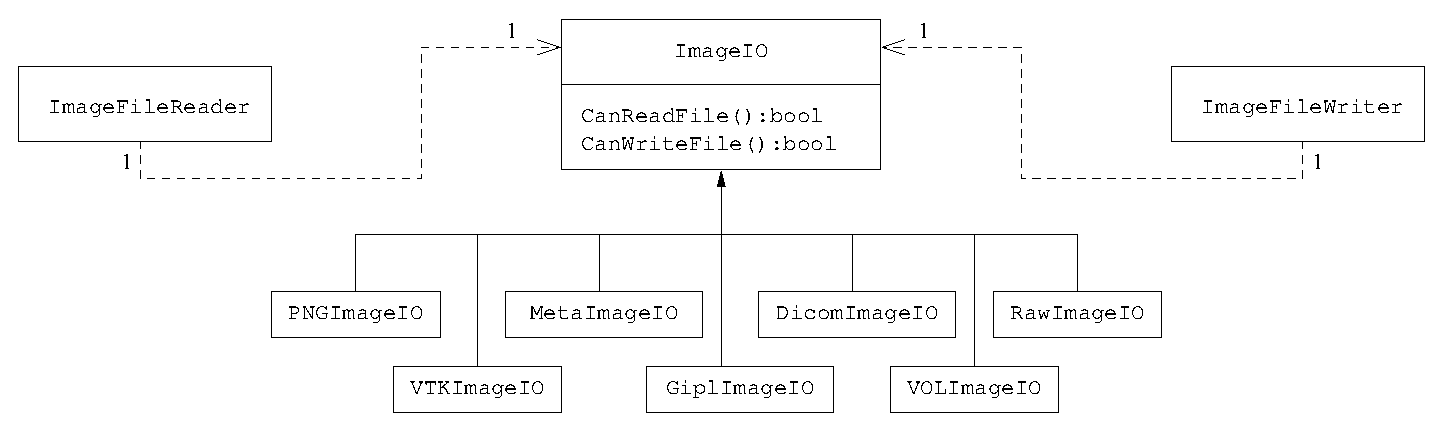
\includegraphics[width=\textwidth]{ImageIOCollaborationDiagram.eps}
\itkcaption[Collaboration diagram of the ImageIO classes]{Collaboration diagram
of the ImageIO classes.} \label{fig:ImageIOCollaborationDiagram}
\end{figure}

\begin{figure}
\center
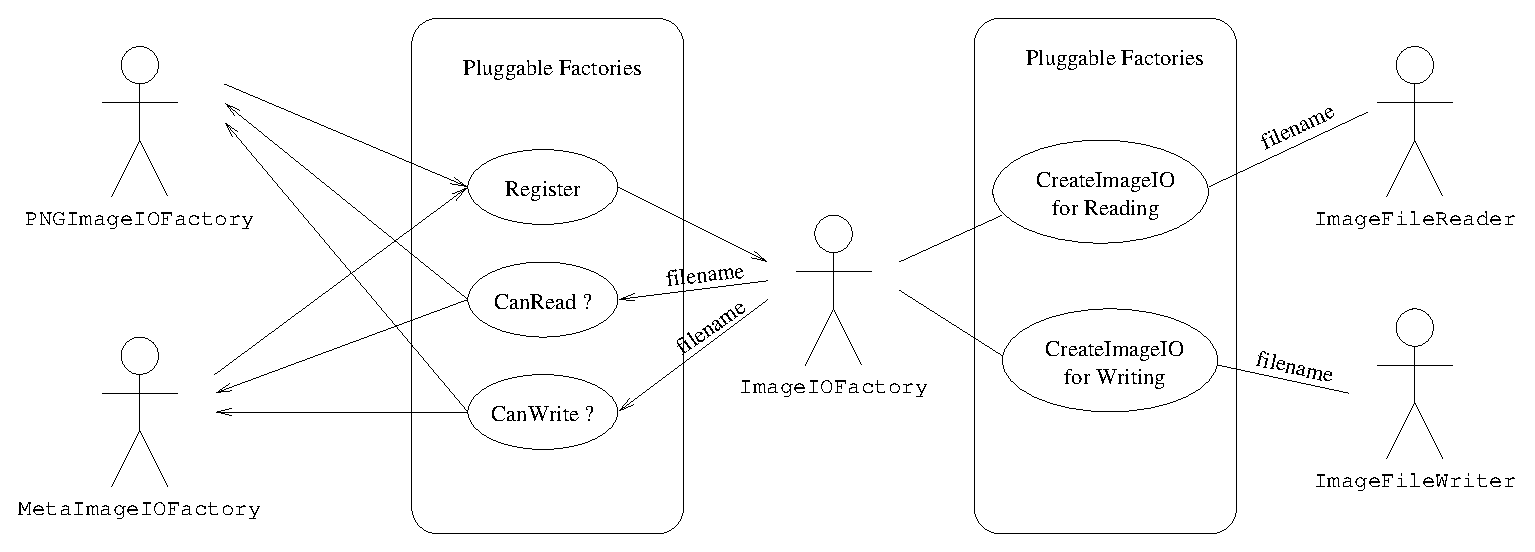
\includegraphics[width=\textwidth]{ImageIOFactoriesUseCases.eps}
\itkcaption[Use cases of ImageIO factories] {Use cases of ImageIO factories.}
\label{fig:ImageIOFactoriesUseCases}
\end{figure}

\begin{figure}
\center
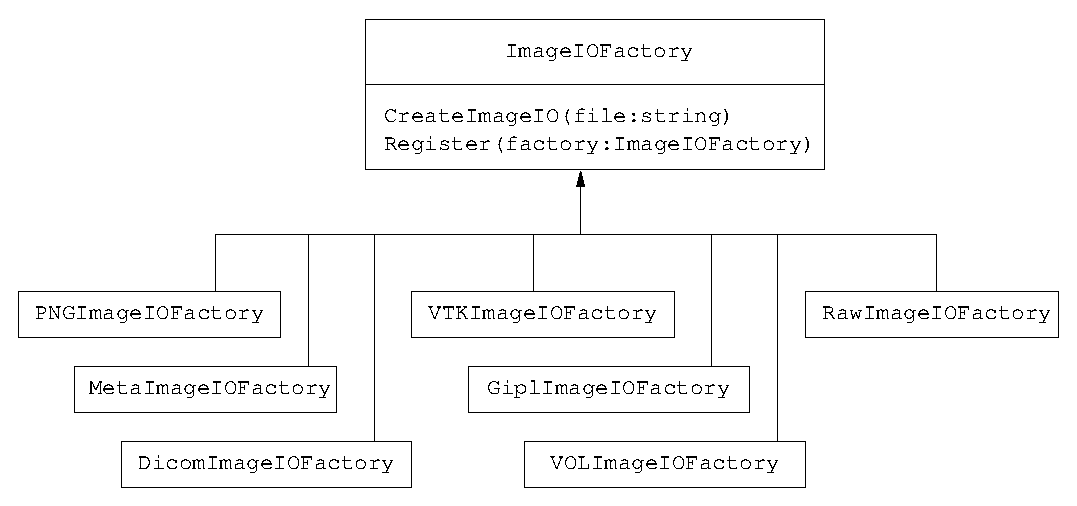
\includegraphics[width=\textwidth]{ImageIOFactoriesClassDiagram.eps}
\itkcaption[Class diagram of ImageIO factories] {Class diagram of the ImageIO
factories.}
\label{fig:ImageIOFactoriesClassDiagram}
\end{figure}


The following section describes the internals of the IO architecture provided
in the toolkit.

\section{Pluggable Factories}
\label{sec:ImageIOPluggableFactories}

The principle behind the input/output mechanism used in ITK is known as
\emph{pluggable-factories} \cite{Gamma1995}. This concept is illustrated in
the UML diagram in Figure~\ref{fig:ImageIOCollaborationDiagram}. From the
user's point of view the objects responsible for reading and writing files
are the \doxygen{ImageFileReader} and \doxygen{ImageFileWriter}
classes. These two classes, however, are not aware of the details involved in
reading or writing particular file formats like PNG or DICOM.  What they do
is to dispatch the user's requests to a set of specific classes that are
aware of the details of image file formats. These classes are the
\doxygen{ImageIO} classes. The ITK delegation mechanism enables users to
extend the number of supported file formats by just adding new classes to the
ImageIO hierarchy.

Each instance of ImageFileReader and ImageFileWriter has
a pointer to an ImageIO object. If this pointer is empty, it will
be impossible to read or write an image and the image file reader/writer must
determine which ImageIO class to use to perform IO operations.
This is done basically by passing the filename to a centralized class, the
\doxygen{ImageIOFactory} and asking it to identify any subclass of
ImageIO capable of reading or writing the user-specified file. This
is illustrated by the use cases on the right side of
Figure~\ref{fig:ImageIOFactoriesUseCases}. The ImageIOFactory acts here as a
dispatcher that help to locate the actual IO factory classes corresponding to
each file format.

Each class derived from ImageIO must provide an associated factory
class capable of producing an instance of the ImageIO class. For
example, for PNG files, there is a \doxygen{PNGImageIO} object that knows how
to read this image files and there is a \doxygen{PNGImageIOFactory} class
capable of constructing a PNGImageIO object and returning a pointer
to it.  Each time a new file format is added (i.e., a new ImageIO
subclass is created), a factory must be implemented as a derived class of the
ObjectFactoryBase class as illustrated in
Figure~\ref{fig:ImageIOFactoriesClassDiagram}.

For example, in order to read PNG files, a PNGImageIOFactory is
created and registered with the central ImageIOFactory
singleton\footnote{\emph{Singleton} means that there is only one instance of
this class in a particular application} class as illustrated in the left side
of Figure~\ref{fig:ImageIOFactoriesUseCases}. When the ImageFileReader asks
the ImageIOFactory for an ImageIO capable of reading the
file identified with \emph{filename} the ImageIOFactory will iterate over the
list of registered factories and will ask each one of them is they know how
to read the file. The factory that responds affirmatively will be used to
create the specific ImageIO instance that will be returned to the
ImageFileReader and used to perform the read operations.

In most cases the mechanism is transparent to the user who only interacts
with the ImageFileReader and ImageFileWriter. It is
possible, however, to explicitly select the type of ImageIO object
to use.  This is illustrated by the following example.

\section{Using ImageIO Classes Explicitly}
\label{sec:ImageReadExportVTK}
\input{ImageReadExportVTK.tex}


\section{Reading and Writing RGB Images}
\label{sec:RGBImagReadWrite}
\input{RGBImageReadWrite.tex}

\section{Reading, Casting and Writing Images}
\label{sec:ImagReadCastWrite}
\input{ImageReadCastWrite.tex}

\section{Extracting Regions}
\label{sec:ImagReadRegionOfInterestWrite}
\input{ImageReadRegionOfInterestWrite.tex}

\section{Extracting Slices}
\label{sec:ImagReadExtractWrite}
\input{ImageReadExtractWrite.tex}


\section{Reading and Writing Vector Images}
\label{sec:VectorImagReadWrite}

Images whose pixel type is a Vector, a CovariantVector, an Array, or a Complex
are quite common in image processing. It is convenient then to describe rapidly
how those images can be saved into files and how they can be read from those
files later on.

\subsection{The Minimal Example}
\label{VectorImageReadWrite}
\input{VectorImageReadWrite.tex}

\subsection{Producing and Writing Covariant Images}
\label{CovariantVectorImageWrite}
\input{CovariantVectorImageWrite.tex}

\subsection{Reading Covariant Images}
\label{CovariantVectorImageRead}
Let's now take the image that we just created and read it into another program.
\input{CovariantVectorImageRead.tex}


\section{Reading and Writing Complex Images}
\label{sec:ComplexImagReadWrite}
\input{ComplexImageReadWrite.tex}


\section{Extracting Components from Vector Images}
\label{sec:VectorImageExtractComponent}
\input{CovariantVectorImageExtractComponent.tex}


\section{Reading and Writing Image Series}

It is still quite common to store 3D medical images in sets of files each one
containing a single slice of a volume dataset. Those 2D files can be read as
individual 2D images, or can be grouped together in order to reconstruct a 3D
dataset. The same practice can be extended to higher dimensions, for example,
for managing 4D datasets by using sets of files each one containing a 3D image.
This practice is common in the domain of cardiac imaging, perfusion, functional
MRI and PET. This section illustrates the functionalities available in ITK for
dealing with reading and writing series of images.

\index{Series!Reading}
\index{Series!Writing}
\index{Image Series!Reading}
\index{Image Series!Writing}

\subsection{Reading Image Series}
\label{sec:ReadingImageSeries}
\input{ImageSeriesReadWrite.tex}

\subsection{Writing Image Series}
\label{sec:WritingImageSeries}
\input{ImageReadImageSeriesWrite.tex}

\subsection{Reading and Writing Series of RGB Images}
\label{sec:ReadingWritingRGBImageSeries}
\input{RGBImageSeriesReadWrite.tex}


\section{Reading and Writing DICOM Images}
\label{sec:ReadingDicomImageSeries2}

% Small intro to DICOM file format
\index{DICOM}
\index{DICOM!Standard}
\index{DICOM!Series}
\index{DICOM!Introduction}

\subsection{Foreword}
With the introduction of computed tomography (CT) followed by other digital
diagnostic imaging modalities such as MRI in the 1970's, and the increasing use
of computers in clinical applications, the American College of Radiology
(ACR)\footnote{\url{http://www.acr.org}} and the National Electrical
Manufacturers Association (NEMA)\footnote{\url{http://www.nema.org}} recognized
the need for a standard method for transferring images as well as associated
information between devices manufactured from various vendors.

ACR and NEMA formed a joint committee to develop a standard for Digital Imaging
and Communications in Medicine (DICOM).  This standard was developed in liaison
with other Standardization Organizations such as CEN TC251, JIRA including
IEEE, HL7 and ANSI USA as reviewers.

DICOM is a comprehensive set of standards for handling, storing and
transmitting information in medical imaging. The DICOM standard was developed
based on the previous NEMA specification.  The standard specifies a file format
definition as well as a network communication protocol. DICOM was developed to
enable integration of scanners, servers, workstations and network hardware from
multiple vendors into an image archiving and communication system.

DICOM files consist of a header and a body of image data. The header contains
standardized as well as free-form fields. The set of standardized fields is
called the public DICOM dictionary, an instance of this dictionary is available
in ITK in the file~\code{Insight/Utilities/gdcm/Dict/dicomV3.dic}.  The list of
free-form fields is also called the \emph{shadow dictionary}.

A single DICOM file can contain multiples frames, allowing storage of volumes
or animations. Image data can be compressed using a large variety of standards,
including JPEG (both lossy and lossless), LZW (Lempel Ziv Welch), and RLE
(Run-length encoding).

The DICOM Standard is an evolving standard and it is maintained in accordance
with the Procedures of the DICOM Standards Committee. Proposals for
enhancements are forthcoming from the DICOM Committee member organizations
based on input from users of the Standard. These proposals are considered for
inclusion in future editions of the Standard. A requirement in updating the
Standard is to maintain effective compatibility with previous editions.

For a more detailed description of the DICOM standard see~\cite{DICOMStandard}.

The following sections illustrate how to use the functionalities that ITK
provides for reading and writing DICOM files. This is extremely important in
the domain of medical imaging since most of the images that are acquired a
clinical setting are stored and transported using the DICOM standard.

DICOM functionalities in ITK are provided by the GDCM library. This open source
library was developed by the CREATIS
Team~\footnote{\url{http://www.creatis.insa-lyon.fr}} at
INSA-Lyon~\cite{CreatisINSA-Lyon}.  Although originally this library was
distributed under a LGPL
License\footnote{\url{http://www.gnu.org/copyleft/lesser.html}}, the CREATIS Team was
lucid enough to understand the limitations of that license and agreed to adopt
the more open BSD-like
License\footnote{\url{http://www.opensource.org/licenses/bsd-license.php}}.
This change in their licensing made possible to distribute GDCM
along with ITK.

GDCM is now maintained by Mathieu Malaterre and the GDCM community.
The version distributed with ITK gets updated with major releases of the GDCM
library.

\subsection{Reading and Writing a 2D Image}
\label{DicomImageReadWrite}
\input{DicomImageReadWrite.tex}

\subsection{Reading a 2D DICOM Series and Writing a Volume}
\label{DicomSeriesReadImageWrite2}
\input{DicomSeriesReadImageWrite2.tex}

\subsection{Reading a 2D DICOM Series and Writing a 2D DICOM Series}
\label{DicomSeriesReadSeriesWrite}
\input{DicomSeriesReadSeriesWrite.tex}

\subsection{Printing DICOM Tags From One Slice}
\label{DicomImageReadPrintTags}
\input{DicomImageReadPrintTags.tex}

\subsection{Printing DICOM Tags From a Series}
\label{DicomSeriesReadPrintTags}
\input{DicomSeriesReadPrintTags.tex}

\subsection{Changing a DICOM Header}
\label{DicomImageReadChangeHeaderWrite}
\input{DicomImageReadChangeHeaderWrite.tex}

\chapter{Filtering}

This chapter introduces the most commonly used filters found in the toolkit.
Most of these filters are intended to process images. They will accept one or
more images as input and will produce one or more images as output. ITK is
based on a data pipeline architecture in which the output of one filter is
passed as input to another filter. (See the Data Processing Pipeline section
in Book 1 for more information.)


\section{Thresholding}
\ifitkFullVersion
\label{sec:ThresholdingFiltering}
\fi

The thresholding operation is used to change or identify pixel values based
on specifying one or more values (called the \emph{threshold} value). The
following sections describe how to perform thresholding operations using
ITK.

\subsection{Binary Thresholding}
\label{sec:BinaryThresholdingImageFilter}

\ifitkFullVersion
\input{BinaryThresholdImageFilter.tex}
\fi

\subsection{General Thresholding}
\label{sec:ThresholdingImageFilter}

\ifitkFullVersion
\input{ThresholdImageFilter.tex}
\fi


\section{Edge Detection}

\subsection{Canny Edge Detection}
\ifitkFullVersion
\input{CannyEdgeDetectionImageFilter.tex}
\fi


\section{Casting and Intensity Mapping}
\label{sec:CastingImageFilters}

The filters discussed in this section perform pixel-wise intensity mappings.
Casting is used to convert one pixel type to another, while intensity mappings
also take into account the different intensity ranges of the pixel types.

\subsection{Linear Mappings}
\label{sec:IntensityLinearMapping}

\ifitkFullVersion
\input{CastingImageFilters.tex}
\fi

\subsection{Non Linear Mappings}
\label{sec:IntensityNonLinearMapping}

The following filter can be seen as a variant of the casting filters. Its main
difference is the use of a smooth and continuous transition function of
non-linear form.

\ifitkFullVersion
\input{SigmoidImageFilter.tex}
\fi


\section{Gradients}
\label{sec:GradientFiltering}

Computation of gradients is a fairly common operation in image processing. The
term ``gradient'' may refer in some contexts to the gradient vectors and in
others to the magnitude of the gradient vectors. ITK filters attempt to
reduce this ambiguity by including the \emph{magnitude} term when
appropriate. ITK provides filters for computing both the image of gradient
vectors and the image of magnitudes.

\subsection{Gradient Magnitude}
\label{sec:GradientMagnitudeImageFilter}

\ifitkFullVersion
\input{GradientMagnitudeImageFilter.tex}
\fi

\subsection{Gradient Magnitude With Smoothing}
\label{sec:GradientMagnitudeRecursiveGaussianImageFilter}

\ifitkFullVersion
\input{GradientMagnitudeRecursiveGaussianImageFilter.tex}
\fi


\subsection{Derivative Without Smoothing}
\label{sec:DerivativeImageFilter}

\ifitkFullVersion
\input{DerivativeImageFilter.tex}
\fi


\section{Second Order Derivatives}
\label{sec:SecondOrderDerivatives}


\subsection{Second Order Recursive Gaussian}
\label{sec:SecondDerivativeRecursiveGaussian}

\ifitkFullVersion
\input{SecondDerivativeRecursiveGaussianImageFilter.tex}
\fi


\subsection{Laplacian Filters}
\label{sec:LaplacianFilters}

\subsubsection{Laplacian Filter Finite Difference}
\subsubsection{Laplacian Filter Recursive Gaussian}
\ifitkFullVersion
\input{LaplacianRecursiveGaussianImageFilter1.tex}
\input{LaplacianRecursiveGaussianImageFilter2.tex}
\fi



\section{Neighborhood Filters}
\label{sec:NeighborhoodFilters}

The concept of locality is frequently encountered in image processing in the
form of filters that compute every output pixel using information from a small
region in the neighborhood of the input pixel.  The classical form of
these filters are the $3 \times 3$ filters in 2D images. Convolution masks
based on these neighborhoods can perform diverse tasks ranging from noise
reduction, to differential operations, to mathematical morphology.

The Insight toolkit implements an elegant approach to neighborhood-based image
filtering.  The input image is processed using a special iterator called the
\doxygen{NeighborhoodIterator}. This iterator is capable of moving over all the
pixels in an image and, for each position, it can address the pixels in a local
neighborhood. Operators are defined that apply an algorithmic operation in the
neighborhood of the input pixel to produce a value for the output pixel.  The
following section describes some of the more commonly used filters that take
advantage of this construction. (See the Iterators chapter
in Book 1 for more information.)

\subsection{Mean Filter}
\label{sec:MeanFilter}

\ifitkFullVersion
\input{MeanImageFilter.tex}
\fi

\subsection{Median Filter}
\label{sec:MedianFilter}

\ifitkFullVersion
\input{MedianImageFilter.tex}
\fi


\subsection{Mathematical Morphology}
\label{sec:MathematicalMorphology}

Mathematical morphology has proved to be a powerful resource for image
processing and analysis \cite{Serra1982}. ITK implements mathematical
morphology filters using NeighborhoodIterators and
\doxygen{NeighborhoodOperator}s.  The toolkit contains two types of image
morphology algorithms, filters that operate on binary images and filters that
operate on grayscale images.

\subsubsection{Binary Filters}
\label{sec:MathematicalMorphologyBinaryFilters}

\ifitkFullVersion
\input{MathematicalMorphologyBinaryFilters.tex}
\fi


\subsubsection{Grayscale Filters}
\label{sec:MathematicalMorphologyGrayscaleFilters}

\ifitkFullVersion
\input{MathematicalMorphologyGrayscaleFilters.tex}
\fi


\subsection{Voting Filters}
\label{sec:VotingFilters}

Voting filters are quite a generic family of filters. In fact, both the Dilate
and Erode filters from Mathematical Morphology are very particular cases of the
broader family of voting filters. In a voting filter, the outcome of a pixel is
decided by counting the number of pixels in its neighborhood and applying a
rule to the result of that counting.For example, the typical implementation of
Erosion in terms of a voting filter will be to say that a foreground pixel will
become background if the numbers of background neighbors is greater or equal
than 1. In this context, you could imagine variations of Erosion in which the
count could be changed to require at least 3 foreground.

\subsubsection{Binary Median Filter}

One of the particular cases of Voting filters is the BinaryMedianImageFilter.
This filter is equivalent to applying a Median filter over a binary image. The
fact of having a binary image as input makes possible to optimize the execution
of the filter since there is no real need for sorting the pixels according to
their frequency in the neighborhood.

\ifitkFullVersion
\input{BinaryMedianImageFilter.tex}
\fi

The typical effect of median filtration on a noisy digital image is a dramatic reduction in impulse noise spikes. The filter also tends to preserve brightness differences across signal steps, resulting in reduced blurring of regional boundaries. The filter also tends to preserve the positions of boundaries in an image.

Figure \ref{fig:BinaryMedianImageFilterOutputMultipleIterations} below shows the effect of running the median filter with a 3x3 classical window size
1, 10 and 50 times. There is a tradeoff in noise reduction and the sharpness of the image when the window size is increased\begin{figure}
  \center
  
\includegraphics[width=0.44\textwidth]{BinaryMedianImageFilterOutput1.eps}
  
\includegraphics[width=0.44\textwidth]{BinaryMedianImageFilterOutput10.eps}
  
\includegraphics[width=0.44\textwidth]{BinaryMedianImageFilterOutput50.eps}
  \itkcaption[Effect of many iterations on the BinaryMedian filter.]{Effect of 1, 10 and 50 iterations of the
  BinaryMedianImageFilter using a 3x3 window.}
  \label{fig:BinaryMedianImageFilterOutputMultipleIterations}
\end{figure}.


\subsubsection{Hole Filling Filter}

Another variation of Voting filters is the Hole Filling filter. This filter
converts background pixels into foreground only when the number of foreground
pixels is a majority of the neighbors. By selecting the size of the majority,
this filter can be tuned to fill-in holes of different size. To be more
precise, the effect of the filter is actually related to the curvature of the
edge in which the pixel is located.

\ifitkFullVersion
\input{VotingBinaryHoleFillingImageFilter.tex}
\fi


\subsubsection{Iterative Hole Filling Filter}

The Hole Filling filter can be used in an iterative way, by applying it
repeatedly until no pixel changes. In this context, the filter can be seen as a
binary variation of a Level Set filter.

\ifitkFullVersion
\input{VotingBinaryIterativeHoleFillingImageFilter.tex}
\fi

\section{Smoothing Filters}
\label{sec:SmoothingFilters}

Real image data has a level of uncertainty that is manifested in the
variability of measures assigned to pixels. This uncertainty is usually
interpreted as noise and considered an undesirable component of the image
data. This section describes several methods that can be applied to reduce
noise on images.

\subsection{Blurring}
\label{sec:BlurringFilters}

Blurring is the traditional approach for removing noise from images. It is
usually implemented in the form of a convolution with a kernel. The effect of
blurring on the image spectrum is to attenuate high spatial
frequencies.  Different kernels attenuate frequencies in different ways. One
of the most commonly used kernels is the Gaussian. Two implementations of
Gaussian smoothing are available in the toolkit. The first one is based on a
traditional convolution while the other is based on the application of IIR
filters that approximate the convolution with a Gaussian
\cite{Deriche1990,Deriche1993}.

\subsubsection{Discrete Gaussian}
\label{sec:DiscreteGaussianImageFilter}

\ifitkFullVersion
\input{DiscreteGaussianImageFilter.tex}
\fi


\subsubsection{Binomial Blurring}
\label{sec:BinomialBlurImageFilter}

\ifitkFullVersion
\input{BinomialBlurImageFilter.tex}
\fi

\subsubsection{Recursive Gaussian IIR}
\label{sec:RecursiveGaussianImageFilter}

\ifitkFullVersion
\input{SmoothingRecursiveGaussianImageFilter.tex}
\fi


\subsection{Local Blurring}
\label{sec:BlurringFunctions}

In some cases it is desirable to compute smoothing in restricted regions of the
image, or to do it using different parameters that are computed locally.  The
following sections describe options for applying local smoothing in images.

\subsubsection{Gaussian Blur Image Function}
\label{sec:GaussianBlurImageFunction}

\ifitkFullVersion
\input{GaussianBlurImageFunction.tex}
\fi

\subsection{Edge Preserving Smoothing}
\label{sec:EdgePreservingSmoothingFilters}

\subsubsection{Introduction to Anisotropic Diffusion}
\label{sec:IntroductionAnisotropicDiffusion}
\ifitkFullVersion
%
%
%  This file in inserted in the Filtering.tex file.
%
%

The drawback of image denoising (smoothing) is that it tends to blur away the
sharp boundaries in the image that help to distinguish between the
larger-scale anatomical structures that one is trying to characterize (which
also limits the size of the smoothing kernels in most applications).  Even in
cases where smoothing does not obliterate boundaries, it tends to distort the
fine structure of the image and thereby changes subtle aspects of the
anatomical shapes in question.

Perona and Malik \cite{Perona1990} introduced an alternative to
linear-filtering that they called \emph{anisotropic diffusion}.  Anisotropic
diffusion is closely related to the earlier work of Grossberg
\cite{Grossberg1984}, who used similar nonlinear diffusion processes to model
human vision.  The motivation for anisotropic diffusion (also called
\emph{nonuniform} or \emph{variable conductance} diffusion) is that a Gaussian
smoothed image is a single time slice of the solution to the heat equation,
that has the original image as its initial conditions.  Thus, the solution to
\begin{equation} \frac{\partial g(x, y, t) }{\partial t} = \nabla \cdot \nabla
g(x, y, t), \end{equation} where $g(x, y, 0) = f(x, y)$ is the input image, is
$g(x, y, t) = G(\sqrt{2t}) \otimes f(x, y)$, where $G(\sigma)$ is a Gaussian
with standard deviation $\sigma$.

Anisotropic diffusion includes a variable conductance term that, in turn,
depends on the differential structure of the image.  Thus, the variable
conductance can be formulated to limit the smoothing at ``edges'' in images, as
measured by high gradient magnitude, for example. \begin{equation} g_{t} = \nabla \cdot
c(\left| \nabla g \right|) \nabla g, \label{eq:aniso} \end{equation} where, for
notational convenience, we leave off the independent parameters of $g$ and use
the subscripts with respect to those parameters to indicate partial
derivatives.  The function $c(|\nabla g|)$ is a fuzzy cutoff that reduces the
conductance at areas of large $|\nabla g|$, and can be any one of a number of
functions.  The literature has shown \begin{equation} c(|\nabla g|) =
e^{-\frac{|\nabla g|^{2}}{2k^{2}}} \end{equation} to be quite effective.
Notice that conductance term introduces a free parameter $k$, the {\em
conductance parameter}, that controls the sensitivity of the process to edge
contrast.  Thus, anisotropic diffusion entails two free parameters: the
conductance parameter, $k$, and the time parameter, $t$, that is analogous to
$\sigma$, the effective width of the filter when using Gaussian kernels.

Equation \ref{eq:aniso} is a nonlinear partial differential equation that can
be solved on a discrete grid using finite forward differences.  Thus, the
smoothed image is obtained only by an iterative process, not a convolution or
non-stationary, linear filter.  Typically, the number of iterations required
for practical results are small, and large 2D images can be processed in
several tens of seconds using carefully written code running on modern, general
purpose, single-processor computers.  The technique applies readily and
effectively to 3D images, but requires more processing time.

In the early 1990's several research groups \cite{Gerig1991,Whitaker1993d}
demonstrated the effectiveness of anisotropic diffusion on medical images.  In
a series of papers on the subject
\cite{Whitaker1993,Whitaker1993b,Whitaker1993c,Whitaker1993d,Whitaker-thesis,Whitaker1994},
Whitaker described a detailed analytical and empirical analysis, introduced a
smoothing term in the conductance that made the process more robust, invented a
numerical scheme that virtually eliminated directional artifacts in the
original algorithm, and generalized anisotropic diffusion to vector-valued
images, an image processing technique that can be used on vector-valued medical
data (such as the color cryosection data of the Visible Human Project).

For a vector-valued input $\vec{F}:U \mapsto \Re^{m}$ the process takes the
form \begin{equation} \vec{F}_{t} = \nabla \cdot c({\cal D}\vec{F}) \vec{F},
\label{eq:vector_diff} \end{equation} where ${\cal D}\vec{F}$ is a {\em
dissimilarity} measure of $\vec{F}$, a generalization of the gradient magnitude
to vector-valued images, that can incorporate linear and nonlinear coordinate
transformations on the range of $\vec{F}$.  In this way, the smoothing of the
multiple images associated with vector-valued data is coupled through the
conductance term, that fuses the information in the different images.  Thus
vector-valued, nonlinear diffusion can combine low-level image features (e.g.
edges) across all ``channels'' of a vector-valued image in order to preserve or
enhance those features in all of image ``channels''.

Vector-valued anisotropic diffusion is useful for denoising data from devices
that produce multiple values such as MRI or color photography.  When performing
nonlinear diffusion on a color image, the color channels are diffused
separately, but linked through the conductance term. Vector-valued diffusion
is also useful for processing registered data from different devices or for
denoising higher-order geometric or statistical features from scalar-valued
images \cite{Whitaker1994,Yoo1993}.

The output of anisotropic diffusion is an image or set of images that
demonstrates reduced noise and texture but preserves, and can also enhance,
edges.  Such images are useful for a variety of  processes including
statistical classification, visualization, and geometric feature extraction.
Previous work has shown \cite{Whitaker-thesis} that anisotropic diffusion, over
a wide range of conductance parameters, offers quantifiable advantages over
linear filtering for edge detection in medical images.

Since the effectiveness of nonlinear diffusion was first demonstrated, numerous
variations of this approach have surfaced in the literature \cite{Romeny1994}.
These include alternatives for constructing dissimilarity measures
\cite{Sapiro1996}, directional (i.e., tensor-valued) conductance terms
\cite{Weickert1996,Alvarez1994} and level set interpretations
\cite{Whitaker2001}.

\fi


\subsubsection{Gradient Anisotropic Diffusion}
\label{sec:GradientAnisotropicDiffusionImageFilter}

\ifitkFullVersion
\input{GradientAnisotropicDiffusionImageFilter.tex}
\fi



\subsubsection{Curvature Anisotropic Diffusion}
\label{sec:CurvatureAnisotropicDiffusionImageFilter}

\ifitkFullVersion
\input{CurvatureAnisotropicDiffusionImageFilter.tex}
\fi

\subsubsection{Curvature Flow}
\label{sec:CurvatureFlowImageFilter}

\ifitkFullVersion
\input{CurvatureFlowImageFilter.tex}
\fi

\subsubsection{MinMaxCurvature Flow}
\label{sec:MinMaxCurvatureFlowImageFilter}

\ifitkFullVersion
\input{MinMaxCurvatureFlowImageFilter.tex}
\fi


\subsubsection{Bilateral Filter}
\label{sec:BilateralImageFilter}

\ifitkFullVersion
\input{BilateralImageFilter.tex}
\fi



\subsection{Edge Preserving Smoothing in Vector Images}
\label{sec:VectorAnisotropicDiffusion}

Anisotropic diffusion can also be applied to images whose pixels are vectors.
In this case the diffusion is computed independently for each vector
component.  The following classes implement versions of anisotropic diffusion
on vector images.

\subsubsection{Vector Gradient Anisotropic Diffusion}
\label{sec:VectorGradientAnisotropicDiffusionImageFilter}

\ifitkFullVersion
\input{VectorGradientAnisotropicDiffusionImageFilter.tex}
\fi

\subsubsection{Vector Curvature Anisotropic Diffusion}
\label{sec:VectorCurvatureAnisotropicDiffusionImageFilter}

\ifitkFullVersion
\input{VectorCurvatureAnisotropicDiffusionImageFilter.tex}
\fi



\subsection{Edge Preserving Smoothing in Color Images}
\label{sec:ColorAnisotropicDiffusion}

\subsubsection{Gradient Anisotropic Diffusion}
\label{sec:ColorGradientAnisotropicDiffusion}

\ifitkFullVersion
\input{RGBGradientAnisotropicDiffusionImageFilter.tex}
\fi

\subsubsection{Curvature Anisotropic Diffusion}
\label{sec:ColorCurvatureAnisotropicDiffusion}

\ifitkFullVersion
\input{RGBCurvatureAnisotropicDiffusionImageFilter.tex}
\fi



\section{Distance Map}
\label{sec:DistanceMap}

\ifitkFullVersion
\input{DanielssonDistanceMapImageFilter.tex}
\fi

\ifitkFullVersion
\input{SignedDanielssonDistanceMapImageFilter.tex}
\fi




\section{Geometric Transformations}
\label{sec:GeometricalTransformationFilters}

\subsection{Filters You Should be Afraid to Use}

\label{sec:ScaryImageFilters}
\subsection{Change Information Image Filter}

This one is the scariest and more dangerous filter in the entire toolkit. You
should not use this filter unless you are entirely certain that you know what
you are doing. In fact if you decide to use this filter, you should write your
code, then go for a long walk, get more coffee and ask yourself if you really
needed to use this filter. If the answer is yes, then you should discuss this
issue with someone you trust and get his/her opinion in writing.  In general,
if you need to use this filter, it means that you have a poor image provider
that is putting your career at risk along with the life of any potential
patient whose images you may end up processing.

\subsection{Flip Image Filter}

\ifitkFullVersion
\input{FlipImageFilter.tex}
\fi

\subsection{Resample Image Filter}
\label{sec:ResampleImageFilter}

\subsubsection{Introduction}

\ifitkFullVersion
\input{ResampleImageFilter.tex}
\fi

\subsubsection{Importance of Spacing and Origin}
\ifitkFullVersion
\input{ResampleImageFilter2.tex}
\fi

\subsubsection{A Complete Example}
\ifitkFullVersion
\input{ResampleImageFilter3.tex}
\fi

\subsubsection{Rotating an Image}
\ifitkFullVersion
\input{ResampleImageFilter4.tex}
\fi

\subsubsection{Rotating and Scaling an Image}
\ifitkFullVersion
\input{ResampleImageFilter5.tex}
\fi

\subsubsection{Resampling using a deformation field}
\ifitkFullVersion
\input{WarpImageFilter1.tex}
\fi


\subsubsection{Subsampling and image in the same space}
\label{SubsampleVolume}

\ifitkFullVersion
\input{SubsampleVolume.tex}
\fi



\subsubsection{Resampling an Anisotropic image to make it Isotropic}
\label{ResampleVolumesToBeIsotropic}

\ifitkFullVersion
\input{ResampleVolumesToBeIsotropic.tex}
\fi



\section{Frequency Domain}
\label{sec:FrequencyDomain}


\subsection{Computing a Fast Fourier Transform (FFT)}
\label{FFTImageFilter}

\ifitkFullVersion
\input{FFTImageFilter.tex}
\fi


\subsection{Filtering on the Frequency Domain}
\label{FFTImageFilterFourierDomainFiltering}

\ifitkFullVersion
\input{FFTImageFilterFourierDomainFiltering.tex}
\fi



\section{Extracting Surfaces}
\label{sec:ExtractingSurfaces}

\subsection{Surface extraction}
\label{sec:SufaceExtraction}
\index{Surface Extraction}

\ifitkFullVersion
\input{SurfaceExtraction.tex}
\fi

\chapter{Registration}

\begin{floatingfigure}[rlp]{8cm}
  \centering
  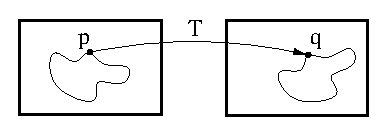
\includegraphics[width=8cm]{ImageRegistrationConcept.eps}
  \caption[Image Registration Concept]{Image registration is the task of
finding a spatial transform mapping on image into
another.\label{fig:ImageRegistrationConcept}}
\end{floatingfigure}

This chapter introduces ITK's capabilities for performing image
registration. Image registration is the process of determining the spatial
transform that maps points from one image to homologous points on a object in
the second image. This concept is schematically represented in Figure
\ref{fig:ImageRegistrationConcept}. In ITK, registration is performed within
a framework of pluggable components that can easily be interchanged.  This
flexibility means that a combinatorial variety of registration methods can be
created, allowing users to pick and choose the right tools for their specific
application.


\section{Registration Framework}
Let's begin with a simplified typical registration framework where its components
and their interconnections are shown in Figure \ref{fig:RegistrationComponents}.
The basic input data to the registration process are two images: one is defined
as the \emph{fixed} image $f(\bf{X})$ and the other as the \emph{moving} image
$m(\bf{X})$. Where $\bf{X}$ represents a position in N-dimensional space.
Registration is treated as an optimization problem with the goal of finding the
spatial mapping that will bring the moving image into alignment with the fixed image.

\begin{figure}
\center
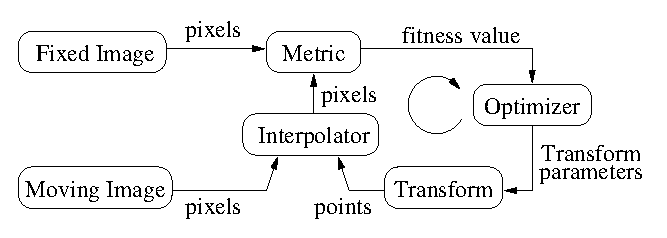
\includegraphics[width=0.8\textwidth]{RegistrationComponentsDiagram.eps}
\itkcaption[A Typical Registration Framework Components]{The basic components
of a typical registration framework are two input images, a transform, a
metric, an interpolator and an optimizer.}
\label{fig:RegistrationComponents}
\end{figure}

The \emph{transform} component $T(\bf{X})$ represents the spatial mapping of
points from the fixed image space to points in the moving image space. The
\emph{interpolator} is used to evaluate moving image intensities at non-grid
positions. The \emph{metric} component $S(f,m \circ T)$ provides a measure of
how well the fixed image is matched by the transformed moving image. This
measure forms the quantitative criterion to be optimized by the
\emph{optimizer} over the search space defined by the parameters of the
\emph{transform}.

The ITKv4 registration framework provides more flexibility to the above traditional
registration concept. In this new framework, specifications of the registration
matching metric comparison locations can be completely different than the pixel
sampling locations in the fixed image.
It means that the registration computations can happen on a physical grid
completely different than the fixed image domain and sampling desity.
This sampling domain can be considered as a new component in the registration
framework that is called \textbf{virtual image}. Moreover, the matching metric
does not need to be computed on a uniform grid of points; it can be computed
on an arbitrary set of physical points.

Various ITKv4 registration components are illustrated in Figure
\ref{fig:ITKv4RegistrationComponents}. Boxes with dashed borders show
\emph{data objects}, while those with solid borders show \emph{process objects}.

\begin{figure}
\center
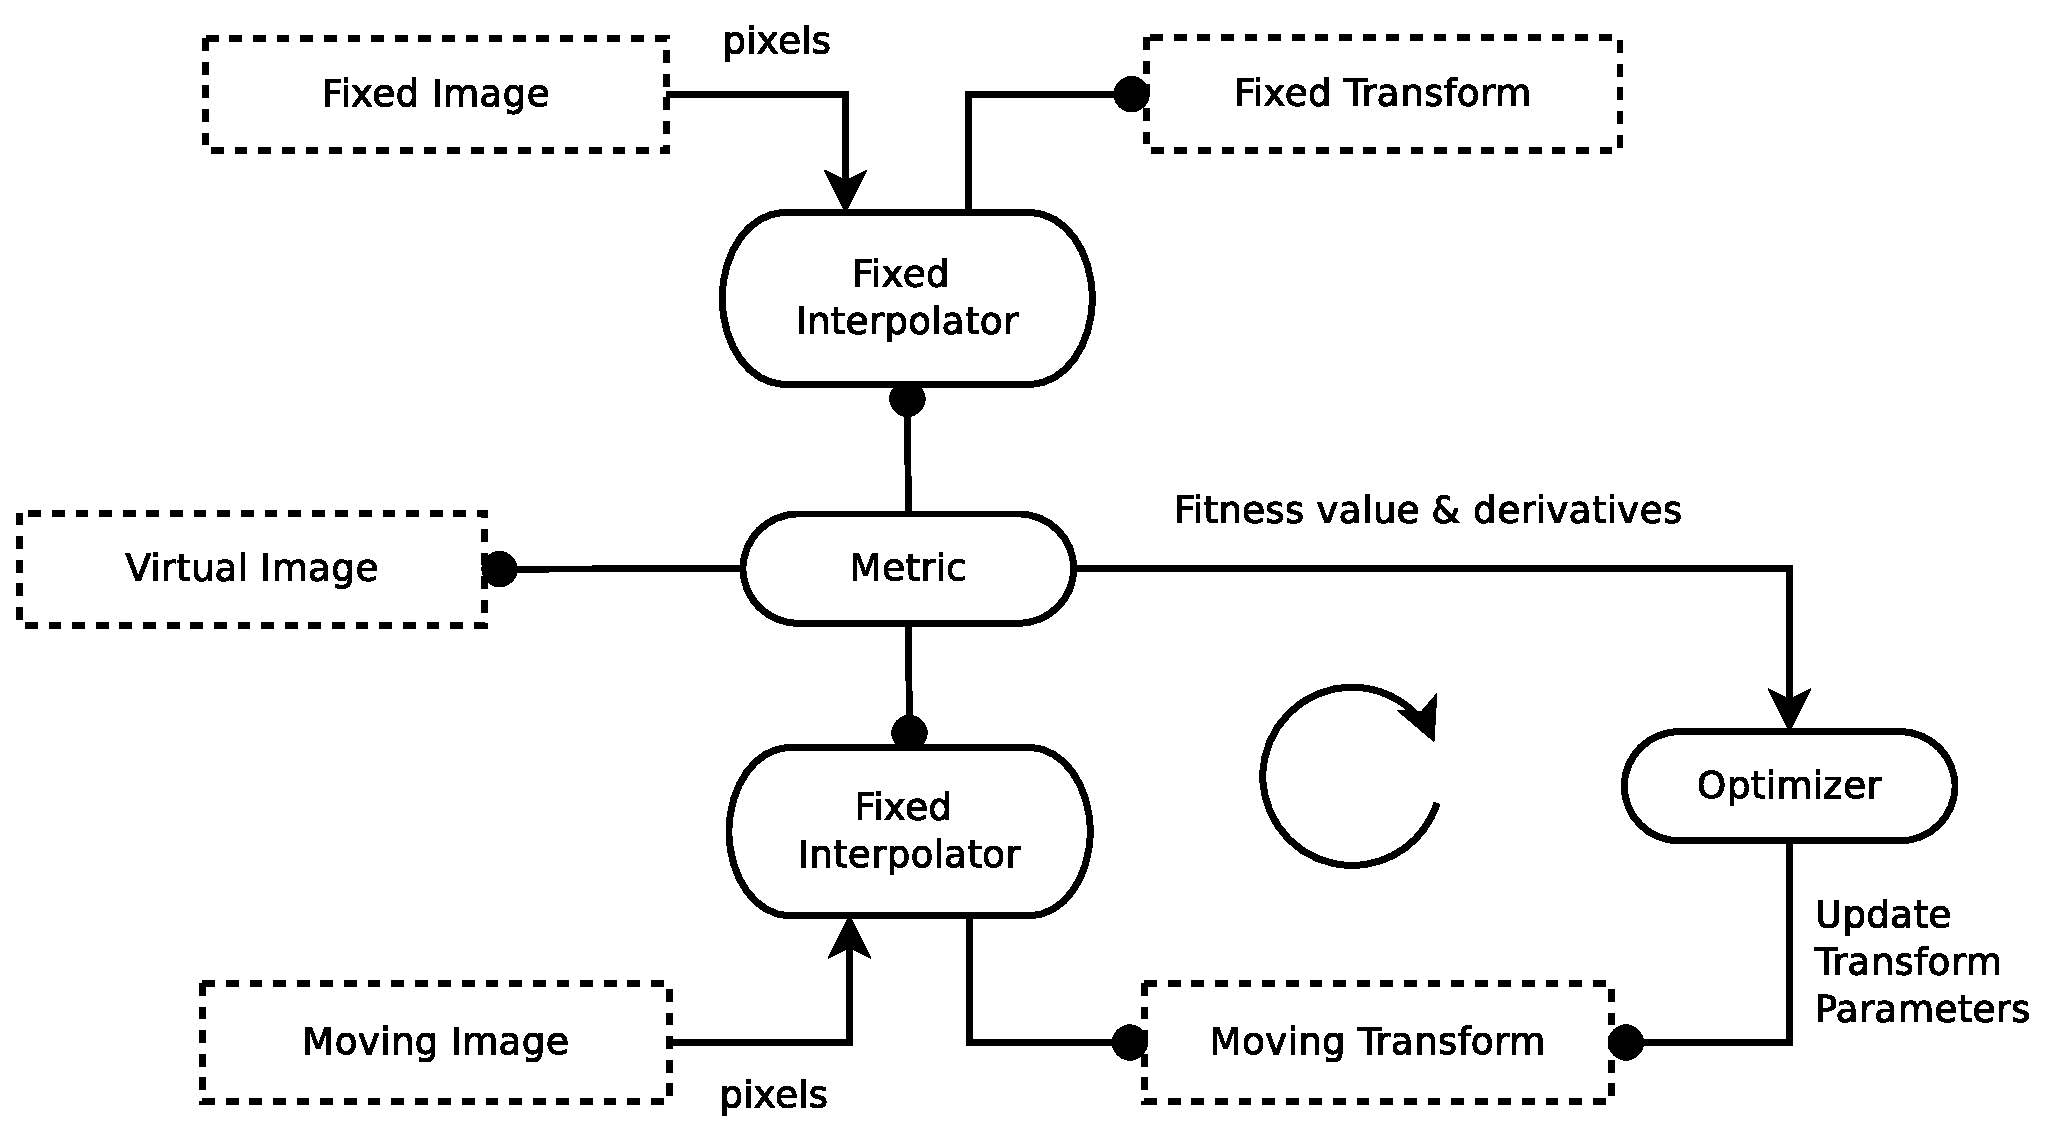
\includegraphics[width=0.8\textwidth]{ITKv4RegistrationComponentsDiagram.eps}
\itkcaption[Registration Framework Components]{The basic components of the ITKv4
registration framework.}
\label{fig:ITKv4RegistrationComponents}
\end{figure}

The matching Metric class is a key component that controls most parts of the
registration process since it handles fixed, moving and virtual images as well
as fixed and moving transforms and interpolators.

Fixed and moving transforms and interpolators are used by the metric to evaluate
the intensity values of the fixed and moving images at each physical point of the
virtual space. Those intensity values are then used by the metric cost function to
evaluate its fitness value and derivatives, which are passed to the optimizer that
asks the moving transform to update its parameters based on the outputs of the cost
function. Since the moving transform is shared between metric and optimizer,
the above process will be repeated till the convergence criteria are met.

Later in section~\ref{sec: FeaturesOfTheRegistrationFramework} you will get a
better understanding of the behind the scene processes of ITKv4 registration
framework. First, we begin with some simple registration examples.


\section{"Hello World" Registration}
\label{sec:IntroductionImageRegistration}
\ifitkFullVersion
\input{ImageRegistration1.tex}
\fi

\section{Features of the Registration Framework}
\label{sec:FeaturesOfTheRegistrationFramework}

This section presents behind the scene of the registration process in ITKv4.
Understanding what actually happens is necessary to have a correct interpretation
of the results of the registration filter. It also helps to understand the
most common difficulties that users encounter when they start using the ITKv4
registration framework that are:

\begin{itemize}
\item The fact that registration is done in physical coordinates
\item The direction of the transform mapping
\end{itemize}

The reason why these two topics tend to create confusion is that they
are implemented in different ways in other systems, and community members tend to
have different expectations regarding how registration should work in ITKv4. The
situation is further complicated by the fact that most people describe image
operations as if they were manually performed on a continues picture on a page
of paper.

These concepts are discussed in this section through a general example shown in
Figure~\ref{fig:ImageRegistrationCoordinateSystemsDiagram}.

\begin{figure}
\center
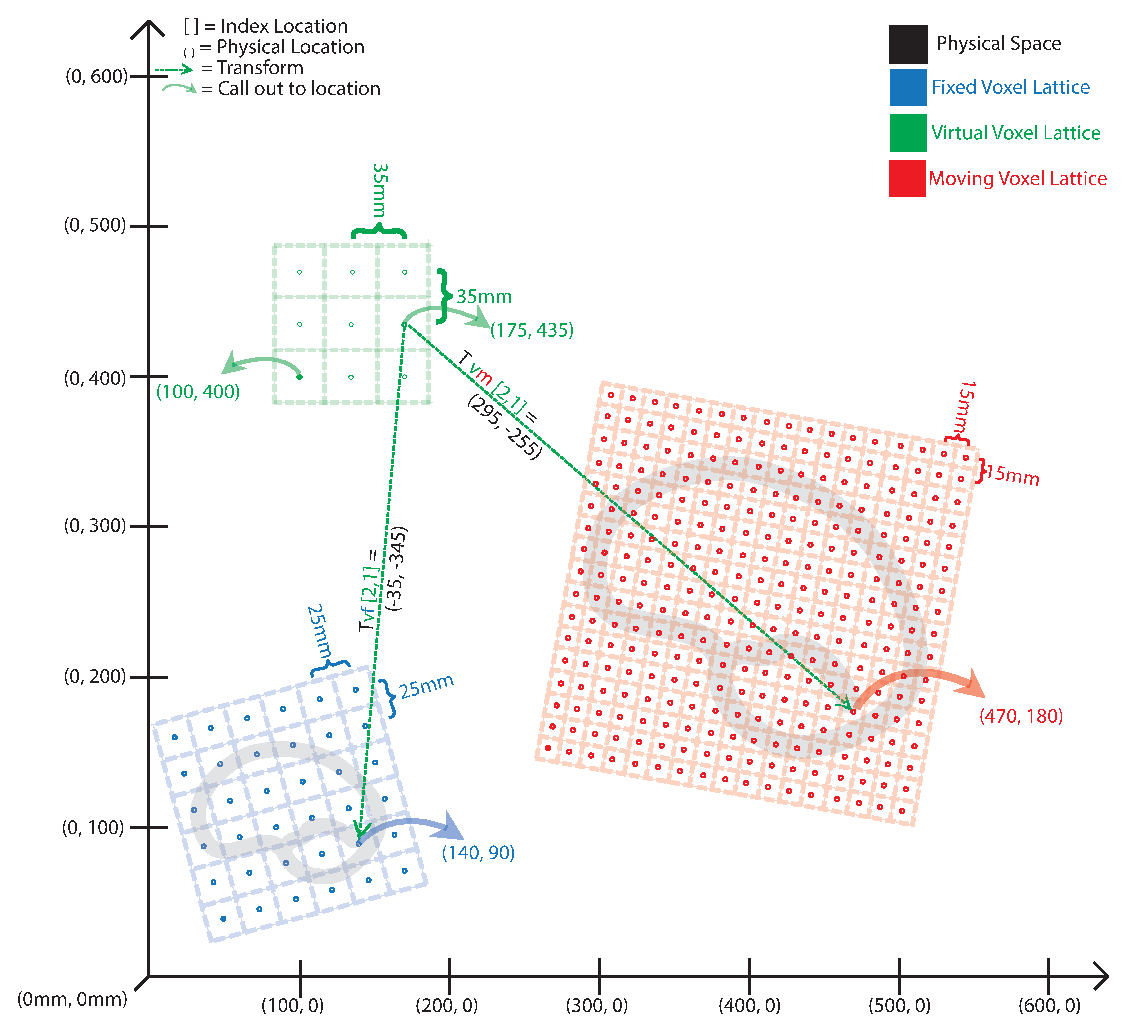
\includegraphics[width=0.75\textwidth]{ImageRegistrationCoordinateSystemsDiagram.eps}
\itkcaption[Registration Coordinate Systems]{Different coordinate systems
involved in the image registration process. Note that the transform being
optimized is the one mapping from the physical space of the \textbf{virtual}
image into the physical space of the \textbf{moving} image.}
\label{fig:ImageRegistrationCoordinateSystemsDiagram}
\end{figure}

Recall that ITKv4 does the registration in ``physical'' space where fixed,
moving and virtual images are placed. Also, note that the term of
virtual image is disceptive here since it does not refer to any actual
image. In fact, the virtual image defines the origin, direction and the
spacing of a space lattice that holds the output resampled image of the
registration process. The virtual pixel lattice is illustrated in green
at the top left side of the example of
Figure~\ref{fig:ImageRegistrationCoordinateSystemsDiagram}.

As shown in this figure, generally there are two transforms involved in the
registration process even though only one of them is being optimized. $T_{vm}$
maps points from physical virtual space onto the physical space of the moving
image, and in the same way $T_{vf}$ finds homologous points between physical
virtual space and the physical space of the fixed image. Note that only
$T_{vm}$ is optimized during the registration process. $T_{vf}$ cannot be
optimized. The fixed transform usually is an identity transform since the
virtual image lattice is commonly defined as the fixed image lattice.

When the registration starts, the algorithm goes through each grid point of the
virtual lattice in a raster sweep. At each point the fixed
and moving transforms find coordinates of the homologous points in the fixed
and moving image physical spaces, and interpolators are used to find the pixel
intensities if mapped points are in non-grid positions. These intensity values
are passed to a cost function to find the current metric value.

Note to the direction of the mapping transforms here. For example,
if you consider the $T_{vm}$ transform, confusion often occurs since
the transform shifts a virtual lattice point on the \textbf{positive}
X direction, the visual effect of this mapping, once the moving
image is resampled, is equivalent to manually shifting the moving
image along the \textbf{negative} X direction. In the same way, when
the $T_{vm}$ transform applies a \textbf{clock-wise} rotation to the
virtual space points, the visual effect of this mapping, once the
moving image has been resampled, is equivalent to manually rotating
the moving image \textbf{counter-clock-wise}. The same relationships
also occur with the $T_{vf}$ transform between the virtual space and
the fixed image space.

This mapping direction is chosen because the moving image is resampled
on the grid of the virtual image. The nature of the resampling process
is such that an algorithm must go through every pixel of the output image
and compute the intensity that should be assigned to this pixel by
mapping to its location in the moving image.

Instead, if we have used the transform that maps coordinates from the
moving image physical space into the virtual image physical space,
then the resampling process could not guarantee that every pixel in
the grid of the virtual image will receive one and only one value.
In other words, the resampling will result in an image with
holes and with redundant or overlapping pixel values.

As seen in the previous examples, and as corroborated in the remaining
examples in this chapter, the transform computed by the registration
framework can be used directly in the resampling filter in order to
map the moving image onto the discrete grid of the virtual image.

There are exceptional cases in which the transform desired is actually
the inverse transform of the one computed by the ITK registration framework.
Only those cases may require invoking the \code{GetInverse()}
method that most transforms offer. Before following that dark path,
read the examples on resampling illustrated in
section~\ref{sec:GeometricalTransformationFilters} in order to get
familiar with the correct interpretation of the transforms.

Now we come back to the situation illustrated in
Figure~\ref{fig:ImageRegistrationCoordinateSystemsDiagram}. This figure shows
the flexibility of the ITKv4 registration framework. We can register two
images with different scales, sizes and resolutions. Also, we can create the
output warped image with any desired size and resolution.

Nevertheless, note that the spatial transform computed during the
registration process does not need to be concerned about a different number
of pixels and different pixel sizes between fixed, moving and output images
because the conversion from index space to the physical space implicitly
takes care of the required scaling factor between the involved images.

One important consequence of this fact is that having the correct image origin,
image pixel size, and image direction is fundamental for the success of the
registration process in ITK, since we need this information to compute the exact
location of each pixel lattice in the physical space; we must make sure
that the correct values for the origin, spacing, and direction of all
fixed, moving and virtual images are provided.

In this example, the spatial transform computed will \textbf{physically} map
the brain from the moving image onto the virtual space and minimizes its
difference with the resampled brain from the fixed image into the virtual
space. Fortunately in practice there is no need to resample the fixed image
since the virtual image physical domain is often assumed to be the same as
physical domain of the fixed image.

\section{Monitoring Registration}
\label{sec:MonitoringImageRegistration}
\ifitkFullVersion
\input{ImageRegistration3.tex}
\fi



\section{Multi-Modality Registration}
\label{sec:MultiModalityRegistration}

Some of the most challenging cases of image registration arise when images of
different modalities are involved. In such cases, metrics based on direct
comparison of gray levels are not applicable. It has been extensively shown
that metrics based on the evaluation of mutual information are well suited for
overcoming the difficulties of multi-modality registration.

\index{itk::Image\-Registration\-Method!Multi-Modality}

The concept of Mutual Information is derived from Information Theory and its
application to image registration has been proposed in different forms by
different groups \cite{Collignon1995,Maes97,Viola1997}, a more detailed review
can be found in \cite{Hajnal2001,Pluim2003}. The Insight Toolkit currently
provides two different implementations of Mutual Information metrics (see
section \ref{sec:Metrics} for details). The following example illustrate the
practical use of one of these metrics.

\subsection{Mattes Mutual Information}
\label{sec:MultiModalityRegistrationMattes}
\ifitkFullVersion
\input{ImageRegistration4.tex}
\fi

% #TODO needs updating to new statistics
% \subsection{Plotting joint histograms}
% \label{sec:JointHistograms}
% \ifitkFullVersion
% \input{ImageRegistrationHistogramPlotter.tex}
% \fi


\section{ Centered Transforms }

The ITK image coordinate origin is typically located in one of the image
corners (see the  Defining Origin and Spacing section of Book 1 for details).
This results in counter-intuitive transform behavior when rotations and scaling
are involved. Users tend to assume that rotations and scaling are performed
around a fixed point at the center of the image.  In order to compensate for
this difference in natural interpretation, the concept of \emph{centered}
transforms have been introduced into the toolkit. The following sections
describe the main characteristics of such transforms.

The introduction of the centered transforms in the Insight Toolkit reflects the
dynamic nature of a software library when it evolves in harmony with the
requests of the community that it serves. This dynamism has, as everything else
in real life, some advantages and some disadvantages. The main advantage is that
when a need is identified by the users, it gets implemented in a matter of days
or weeks.  This capability for rapidly responding to the needs of a community
is one of the major strengths of Open Source software. It has the additional
safety that if the rest of the community does not wish to adopt a particular
change, an isolated user can always implement that change in her local copy of
the toolkit, since all the source code of ITK is available in a Apache 2.0
license\footnote{\url{http://www.opensource.org/licenses/Apache-2.0}} that
does not restrict modification nor distribution of the code, and that does not
impose the assimilation demands of viral licenses such as
GPL\footnote{\url{http://www.gnu.org/copyleft/gpl.html}}.

The main disadvantage of dynamism, is of course, the fact that there is
continuous change and a need for perpetual adaptation. The evolution of
software occurs at different scales, some changes happen to evolve in localized
regions of the code, while from time to time accommodations of a larger scale
are needed. The need for continuous changes is addressed in Extreme Programming
with the methodology of \emph{Refactoring}. At any given point, the structure
of the code may not project the organized and neatly distributed architecture
that may have resulted from a monolithic and static design. There is, after
all, good reasons why living beings can not have straight angles. What you are
about to witness in this section is a clear example of the diversity of species
that flourishes when Evolution is in action~\cite{Darwin1999}.


\subsection{Rigid Registration in 2D}
\label{sec:RigidRegistrationIn2D}
\ifitkFullVersion
\input{ImageRegistration5.tex}
\fi

\subsection{Initializing with Image Moments}
\label{sec:InitializingRegistrationWithMoments}
\ifitkFullVersion
\input{ImageRegistration6.tex}
\fi



\subsection{Similarity Transform in 2D}
\label{sec:SimilarityRegistrationIn2D}
\ifitkFullVersion
\input{ImageRegistration7.tex}
\fi



\subsection{Rigid Transform in 3D}
\label{sec:RigidRegistrationIn3D}
\ifitkFullVersion
\input{ImageRegistration8.tex}
\fi




\subsection{Centered Affine Transform}
\label{sec:CenteredAffineTransform}
\ifitkFullVersion
\input{ImageRegistration9.tex}
\fi




\section{Multi-Resolution Registration}
\label{sec:MultiResolutionRegistration}
Performing image registration using a multi-resolution approach is widely used
to improve speed, accuracy and robustness. The basic idea is that registration
is first performed at a coarse scale where the images have fewer pixels.
The spatial mapping determined at the coarse level is then used to initialize
registration at the next finer scale. This process is repeated until it
reaches the finest possible scale. This coarse-to-fine strategy greatly
improve the registration success rate and also increases robustness
by eliminating local optima at coarser scales. Robustness can be improved
even more by smoothing the images at coarse scales.

In all previous examples we ran the registration process at a single resolution. However,
ITKv4 registration framework is structured to provide a multi-resolution registration
method. For this purpose we only need to define the number of levels as well as the
resolution and smoothness of the input images at each level. The registration filter
smoothes and subsamples the images according to user-defined \emph{ShrinkFactor} and
\emph{SmoothingSigma} vectors.

We now present the multi-resolution capabilities of the framework by
way of an example.

\subsection{Fundamentals}
\ifitkFullVersion
\input{MultiResImageRegistration1.tex}
\fi

\subsection{Parameter Tuning}
\ifitkFullVersion
\input{MultiResImageRegistration2.tex}
\fi

With the completion of these examples, we will now review the main
features of the components forming the registration framework.


% This clearpage command is intended to separate the graphics from previous
% examples from the diagrams of this section. This should prevent the
% registration diagrams from getting mixed with the diagrams for the Geometric
% objects used by the Transforms.
\clearpage

\section{Transforms}
\label{sec:Transforms}
\ifitkFullVersion

\def\tableconfiguration{ | p{3cm} | p{1.8cm} | p{2.5cm} | p{4cm} | }


\index{itk::Transform}

\index{Vector!Geometrical Concept}

In the Insight Toolkit, \doxygen{Transform} objects encapsulate the mapping of
points and vectors from an input space to an output space.  If a transform is
invertible, back transform methods are also provided.  Currently, ITK provides
a variety of transforms from simple translation, rotation and scaling to
general affine and kernel transforms.  Note that, while in this section we
discuss transforms in the context of registration, transforms are general and
can be used for other applications. Some of the most commonly used transforms
will be discussed in detail later. Let's begin by introducing the objects used
in ITK for representing basic spatial concepts.


\subsection{Geometrical Representation}
\label{sec:GeometricalObjects}

\begin{figure}
\center
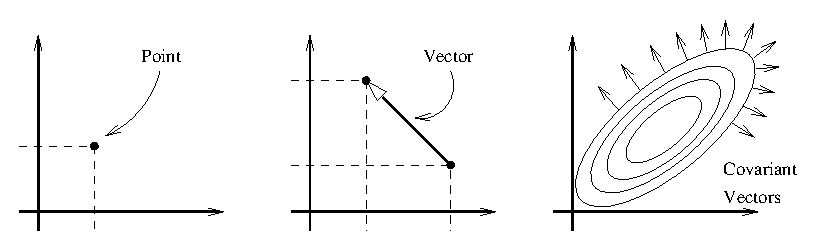
\includegraphics[width=0.9\textwidth]{GeometricalObjects.eps}
\itkcaption[Geometrical representation objects in ITK]{Geometric
representation objects in ITK.}
\label{fig:GeometricalObjects}
\end{figure}
 
ITK implements a consistent geometric representation of the space. The
characteristics of classes involved in this representation are summarized in
Table~\ref{tab:GeometricalConcepts}. In this regard, ITK takes full advantage
of the capabilities of Object Oriented programming and resists the temptation
of using simple arrays of \code{float} or \code{double} in order to represent
geometrical objects. The use of basic arrays would have blurred the important
distinction between the different geometrical concepts and would have allowed
for the innumerable conceptual and programming errors that result from using a
vector where a point is needed or viceversa.

\index{itk::Point!Concept}
\index{itk::Vector!Concept}
\index{itk::CovariantVector!Concept}

\begin{table}
\begin{center}
\begin{tabular}{ | p{0.3\textwidth} | p{ 0.6\textwidth} | }
\hline
\textbf{Class} &
\textbf{Geometrical concept} \\
\hline\hline
\doxygen{Point} & 
Position in space. In $N$-dimensional space it is represented by an array of
$N$ numbers associated with space coordinates. \\
\hline
\doxygen{Vector} & 
Relative position between two points. In $N$-dimensional space it is
represented by an array of $N$ numbers, each one associated with the distance
along a coordinate axis. Vectors do not have a position in space. A vector is
defined as the subtraction of two points.\\
\hline
\doxygen{CovariantVector} & Orthogonal direction to a $(N-1)$-dimensional
manifold in space. For example, in $3D$ it corresponds to the vector orthogonal
to a surface. This is the appropriate class for representing Gradients of
functions. Covariant vectors do not have a position in space. Covariant vector
should not be added to Points, nor to Vectors.\\
\hline
\end{tabular}
\end{center}
\itkcaption[Geometrical Elementary Objects]{Summary of objects representing
geometrical concepts in ITK.\label{tab:GeometricalConcepts}}
\end{table}


Additional uses of the \doxygen{Point}, \doxygen{Vector} and
\doxygen{CovariantVector} classes have been discussed in Chapter
\ref{sec:DataRepresentation}.  Each one of these classes behaves differently
under spatial transformations. It is therefore quite important to keep their
distinction clear. Figure
\ref{fig:GeometricalObjects} illustrates the differences between
these concepts.


\index{itk::Transform!TransformPoint()}
\index{itk::Transform!TransformVector()}
\index{itk::Transform!TransformCovariantVector()}

Transform classes provide different methods for mapping each one of
the basic space-representation objects.  Points, vectors and covariant vectors
are transformed using the methods \code{TransformPoint()},
\code{TransformVector()} and \code{TransformCovariantVector()} respectively.

One of the classes that deserve further comments is the \doxygen{Vector}. This
ITK class tend to be misinterpreted as a container of elements instead of a
geometrical object. This is a common misconception originated by the fact that
Computer Scientist and Software Engineers misuse the term ``Vector''.  The
actual word ``Vector'' is relatively young. It was coined by William Hamilton
in his book ``\emph{Elements of Quaternions}'' published in 1886
(post-mortem)\cite{Hamilton1866}.  In the same text Hamilton coined the terms:
``\emph{Scalar}'', ``\emph{Versor}'' and ``\emph{Tensor}''.  Although the
modern term of ``\emph{Tensor}'' is used in Calculus in a different sense of
what Hamilton defined in his book at the time~\cite{Dodson1997}.

A ``\emph{Vector}'' is, by definition, a mathematical object that embodies the
concept of ``direction in space''. Strictly speaking, a Vector describes the
relationship between two Points in space, and captures both their relative
distance and orientation.

Computer scientists and software engineers missused the term vector in order to
represent the concept of an ``Indexed Set''~\cite{Austern1999}.  Mechanical
Engineers and Civil Engineers, who deal with the real world of physical objects
will not commit this mistake and will keep the word ``\emph{Vector}'' attached
to a geometrical concept.  Biologists, on the other hand, will associate
``\emph{Vector}'' to a ``vehicle'' that allows them to direct something in a
particular direction, for example, a virus that allows them to insert pieces of
code into a DNA strand~\cite{Lodish2000}.

Textbooks in programming do not help to clarify those concepts and losely use
the term ``\emph{Vector}'' for the purpose of representing an ``Enumerated set
of common elements''. STL follows this trend and continue using the word
``\emph{Vector}'' for what it was not supposed to be
used~\cite{Austern1999,Alexandrescu2001}. Linear Algebra devoids the
``\emph{Vector}'' from its notion of Geometrical reality and makes it an
abstract set of numbers with arithmetic operations associated.

For those of you who are looking for the ``\emph{Vector}'' in the Software
Engineering sense, please look at the \doxygen{Array} and \doxygen{FixedArray}
classes that actually provide such functionalities. Additionally, the
\doxygen{VectorContainer} and \doxygen{MapContainer} classes may be of interest
too. These container classes are intended for algorithms that require to insert
and delete elements, and that may have large numbers of elements.

The Insight Toolkit deals with real objects that inhabit the physical space.
This is particularly true in the context of the image registration framework.
We chose to give the appropriate name to the mathematical objects that describe
geometrical relationships in N-Dimensional space. It is for this reason that we
explicitly make clear the distincion between Point, Vector and CovariantVector,
despite the fact that most people would be happy with a simple use of
\code{double[3]} for the three concepts and then will proceed to perform all
sort of conceptually flawed operations such as 

\begin{itemize}
\item Adding two Points
\item Dividing a Point by a Scalar
\item Adding a Covariant Vector to a Point
\item Adding a Covariant Vector to a Vector
\end{itemize}

In order to enforce the correct use of the Geometrical concepts in ITK we
organized these classes in a hierarchy that supports reuse of code and yet
compartamentalize the behavior of the individual classes.  The use of the
\doxygen{FixedArray} as base class of the \doxygen{Point}, the \doxygen{Vector}
and the \doxygen{CovariantVector} was a design decision based on calling things
by their correct name.

An \doxygen{FixedArray} is an enumerated collection with a fixed number of
elements. You can instantiate a fixed array of letters, or a fixed array of
images, or a fixed array of transforms, or a fixed array of geometrical shapes.
Therefore, the FixedArray only implements the functionality that is necesary to
access those enumerated elements. No assumptions can be made at this point on
any other operations required by the elements of the FixedArray, except the
fact of having a default constructor.

The \doxygen{Point} is a type that represents the spatial coordinates of a
spatial location. Based on geometrical concepts we defined the valid operations
of the Point class. In particular we made sure that no \code{operator+()} was
defined between Points, and that no \code{operator*( scalar )} nor
\code{operator/( scalar )} were defined for Points.

In other words, you could do in ITK operations such as:

\begin{itemize}
\item Vector  = Point - Point
\item Point  +=  Vector
\item Point  -=  Vector
\item Point  = BarycentricCombination( Point, Point )
\end{itemize}

and you cannot (because you \textbf{should not}) do operation such as

\begin{itemize}
\item Point = Point * Scalar    
\item Point = Point + Point    
\item Point = Point / Scalar  
\end{itemize}

The \doxygen{Vector} is, by Hamilton's definition, the subtraction between two
points. Therefore a Vector must satisfy the following basic operations:

\begin{itemize}
\item Vector = Point - Point
\item Point  = Point + Vector
\item Point  = Point - Vector
\item Vector = Vector + Vector
\item Vector = Vector - Vector
\end{itemize}

An \doxygen{Vector} object is intended to be instantiated over elements that
support matematical operation such as addition, subtraction and multiplication
by scalars.


\subsection{Transform General Properties}
\label{sec:TransformGeneralProperties}

\index{itk::Transform!SetParameters()} Each transform class typically has
several methods for setting its parameters.  For example,
\doxygen{Euler2DTransform} provides methods for specifying the offset,
angle, and the entire rotation matrix.  However, for use in the
registration framework, the parameters are represented by a flat
Array of doubles to facilitate communication with generic
optimizers. In the case of the Euler2DTransform, the transform is also
defined by three doubles: the first representing the angle, and the last two the
offset. The flat array of parameters is defined using \code{SetParameters()}. A
description of the parameters and their ordering is documented in the 
sections that follow.
 
In the context of registration, the transform parameters define the search
space for optimizers. That is, the goal of the optimization is to find the set
of parameters defining a transform that results in the best possible value of
an image metric. The more parameters a transform has, the longer its
computational time will be when used in a registration method since the
dimension of the search space will be equal to the number of transform
parameters.

\index{itk::Transform!GetJacobian()}

Another requirement that the registration framework imposes on the transform
classes is the computation of their Jacobians. In general, metrics require
the knowledge of the Jacobian in order to compute Metric derivatives.
The Jacobian is a matrix whose element are the partial derivatives of the
output point with respect to the array of parameters that defines the
transform:\footnote{Note that the term \emph{Jacobian} is also commonly used
for the matrix representing the derivatives of output point coordinates with
respect to input point coordinates. Sometimes the term is loosely used to
refer to the determinant of such a matrix.~\cite{Dodson1997}}

\begin{equation}
J=\left[ \begin{array}{cccc}
\frac{\partial x_{1}}{\partial p_{1}} & 
\frac{\partial x_{1}}{\partial p_{2}} & 
\cdots  & \frac{\partial x_{1}}{\partial p_{m}}\\
\frac{\partial x_{2}}{\partial p_{1}} & 
\frac{\partial x_{2}}{\partial p_{2}} & 
\cdots  & \frac{\partial x_{2}}{\partial p_{m}}\\
\vdots  & \vdots  & \ddots  & \vdots \\
\frac{\partial x_{n}}{\partial p_{1}} & 
\frac{\partial x_{n}}{\partial p_{2}} & 
\cdots  & \frac{\partial x_{n}}{\partial p_{m}}
\end{array}\right]
\end{equation}

where $\{p_i\}$ are the transform parameters and $\{x_i\}$ are the coordinates
of the output point.  Within this framework, the Jacobian is represented by an
\doxygen{Array2D} of doubles and is obtained from the transform by method
\code{GetJacobian()}. The Jacobian can be interpreted as a matrix that
indicates for a point in the input space how much its mapping on the output
space will change as a response to a small variation in one of the transform
parameters. Note that the values of the Jacobian matrix depend on the point in
the input space. So actually the Jacobian can be noted as $J(\bf{X})$, where
${\bf{X}}=\{x_i\}$. The use of transform Jacobians enables the efficient
computation of metric derivatives.  When Jacobians are not available, metrics
derivatives have to be computed using finite difference at a price of $2M$
evaluations of the metric value, where $M$ is the number of transform
parameters.

The following sections describe the main characteristics of the transform
classes available in ITK.

\subsection{Identity Transform}
\label{sec:IdentityTransform}
\index{itk::IdentityTransform}

\begin{table}
\begin{center}
\begin{tabular}{\tableconfiguration}
\hline
\textbf{Behavior} &
\textbf{Number of Parameters} &
\textbf{Parameter Ordering} &
\textbf{Restrictions} \\
\hline\hline
Maps every point to itself, every vector to itself and every covariant vector to itself.  & 
0 &
NA  &  
Only defined when the input and output space has the same number of dimensions. \\
\hline
\end{tabular}
\end{center}
\itkcaption[Identity Transform Characteristics]{Characteristics of the identity transform.
\label{tab:IdentityTransformCharacteristics}}
\end{table}

The identity transform \doxygen{IdentityTransform} is mainly used for debugging
purposes. It is provided to methods that require a transform and in cases where
we want to have the certainty that the transform will have no effect whatsoever
in the outcome of the process. It is just a \code{NULL} operation. The main
characteristics of the identity transform are summarized in
Table~\ref{tab:IdentityTransformCharacteristics}


\subsection{Translation Transform}
\label{sec:TranslationTransform}
\index{itk::TranslationTransform}

\begin{table}
\begin{center}
\begin{tabular}{\tableconfiguration}
\hline
\textbf{Behavior} &
\textbf{Number of Parameters} &
\textbf{Parameter Ordering} &
\textbf{Restrictions} \\
\hline\hline
Represents a simple translation of points in the input space
and has no effect on vectors or covariant vectors. &
Same as the input space dimension. &
The $i$-th parameter represents the translation in the $i$-th dimension. &
Only defined when the input and output space has the same number of dimensions. \\
\hline
\end{tabular}
\end{center}
\itkcaption[Translation Transform Characteristics]{Characteristics of the TranslationTransform class.
\label{tab:TranslationTransformCharacteristics}}
\end{table}

The \doxygen{TranslationTransform} is probably the simplest yet one of the most
useful transformations.  It maps all Points by adding a Vector to them.  Vector
and covariant vectors remain unchanged under this transformation since they are
not associated with a particular position in space. Translation is the best
transform to use when starting a registration method. Before attempting to
solve for rotations or scaling it is important to overlap the anatomical
objects in both images as much as possible. This is done by resolving the
translational misalignment between the images. Translations also have the
advantage of being fast to compute and having parameters that are easy to
interpret. The main characteristics of the translation transform are presented
in Table~\ref{tab:TranslationTransformCharacteristics}.

\subsection{Scale Transform}
\label{sec:ScaleTransform}
\index{itk::ScaleTransform}

\begin{table}
\begin{center}
\begin{tabular}{\tableconfiguration}
\hline
\textbf{Behavior} &
\textbf{Number of Parameters} &
\textbf{Parameter Ordering} &
\textbf{Restrictions} \\
\hline\hline
Points are transformed by multiplying each one of their coordinates by the
corresponding scale factor for the dimension.  Vectors are transformed as
points.  Covariant vectors are transformed by \emph{dividing} their components
by the scale factor in the corresponding dimension.  &
Same as the input space dimension. &
The $i$-th parameter represents the scaling in the $i$-th dimension. &
Only defined when the input and output space has the same number of dimensions. \\
\hline
\end{tabular}
\end{center}
\itkcaption[Scale Transform Characteristics]{Characteristics of the ScaleTransform class.
\label{tab:ScaleTransformCharacteristics}}
\end{table}

The \doxygen{ScaleTransform} represents a simple scaling of the
vector space.  Different scaling factors can be applied along each
dimension. Points are transformed by multiplying each one of their
coordinates by the corresponding scale factor for the dimension.  Vectors are
transformed in the same way as points.  Covariant vectors, on the other hand,
are transformed differently since anisotropic scaling does not preserve
angles. Covariant vectors are transformed by \emph{dividing} their components
by the scale factor of the corresponding dimension. In this way, if a
covariant vector was orthogonal to a vector, this orthogonality will be
preserved after the transformation. The following equations summarize the
effect of the transform on the basic geometric objects.

\begin{equation}
\begin{array}{lccccccc}
\mbox{Point }          & \bf{P'} &  =  & T(\bf{P})  & : & \bf{P'}_i &  = & \bf{P}_i \cdot S_i \\
\mbox{Vector}          & \bf{V'} &  =  & T(\bf{V})  & : & \bf{V'}_i &  = & \bf{V}_i \cdot S_i \\
\mbox{CovariantVector} & \bf{C'} &  =  & T(\bf{C})  & : & \bf{C'}_i &  = & \bf{C}_i /     S_i \\
\end{array}
\end{equation}

where $\bf{P}_i$, $\bf{V}_i$ and $\bf{C}_i$ are the point, vector and covariant
vector $i$-th components while $\bf{S}_i$ is the scaling factor along dimension
$i-th$.  The following equation illustrates the effect of the scaling transform
on a $3D$ point.

\begin{equation}
\left[ 
\begin{array}{c}
x' \\
y' \\
z' \\
\end{array}
\right]
=
\left[ 
\begin{array}{ccc}
S_1 &  0  &  0  \\
 0  & S_2 &  0  \\
 0  &  0  & S_3 \\
\end{array}
\right]
\cdot
\left[ 
\begin{array}{c}
x  \\
y  \\
z  \\
\end{array}
\right]
\end{equation}

Scaling appears to be a simple transformation but there are actually a
number of issues to keep in mind when using different scale factors along
every dimension. There are subtle effects---for example, when computing image
derivatives. Since derivatives are represented by covariant vectors, their
values are not intuitively modified by scaling transforms.

One of the difficulties with managing scaling transforms in a registration
process is that typical optimizers manage the parameter space as a vector
space where addition is the basic operation. Scaling is better treated in the
frame of a logarithmic space where additions result in regular multiplicative
increments of the scale. Gradient descent optimizers have trouble updating
step length, since the effect of an additive increment on a scale factor
diminishes as the factor grows. In other words, a scale factor variation of
$(1.0+ \epsilon)$ is quite different from a scale variation of
$(5.0+\epsilon)$.

Registrations involving scale transforms require careful monitoring of the
optimizer parameters in order to keep it progressing at a stable pace. Note
that some of the transforms discussed in following sections, for example, the
AffineTransform, have hidden scaling parameters and are therefore
subject to the same vulnerabilities of the ScaleTransform.

In cases involving misalignments with simultaneous translation, rotation and
scaling components it may be desirable to solve for these components
independently. The main characteristics of the scale transform are presented in
Table~\ref{tab:ScaleTransformCharacteristics}.


\subsection{Scale Logarithmic Transform}
\label{sec:ScaleLogarithmicTransform}
\index{itk::ScaleLogarithmicTransform}

\begin{table}
\begin{center}
\begin{tabular}{\tableconfiguration}
\hline
\textbf{Behavior} &
\textbf{Number of Parameters} &
\textbf{Parameter Ordering} &
\textbf{Restrictions} \\
\hline\hline
Points are transformed by multiplying each one of their coordinates by the
corresponding scale factor for the dimension.  Vectors are transformed as
points.  Covariant vectors are transformed by \emph{dividing} their components
by the scale factor in the corresponding dimension. 
&
Same as the input space dimension. &
The $i$-th parameter represents the scaling in the $i$-th dimension. &
Only defined when the input and output space has the same number of dimensions.
The difference between this transform and the ScaleTransform is that here the
scaling factors are passed as logarithms, in this way their behavior is closer
to the one of a Vector space.  \\
\hline
\end{tabular}
\end{center}
\itkcaption[Scale Logarithmic Transform Characteristics]{Characteristics of the ScaleLogarithmicTransform class.
\label{tab:ScaleLogarithmicTransformCharacteristics}}
\end{table}

The \doxygen{ScaleLogarithmicTransform} is a simple variation of the
\doxygen{ScaleTransform}. It is intended to improve the behavior of the scaling
parameters when they are modified by optimizers. The difference between this
transform and the ScaleTransform is that the parameter factors are passed here
as logarithms. In this way, multiplicative variations in the scale become
additive variations in the logarithm of the scaling factors.




\subsection{Euler2DTransform}
\label{sec:Euler2DTransform}
\index{itk::Euler2DTransform}

\begin{table}
\begin{center}
\begin{tabular}{\tableconfiguration}
\hline
\textbf{Behavior} &
\textbf{Number of Parameters} &
\textbf{Parameter Ordering} &
\textbf{Restrictions} \\
\hline\hline
Represents a $2D$ rotation and a $2D$ translation. Note that the translation
component has no effect on the transformation of vectors and covariant vectors. &
3 &
The first parameter is the angle in radians and the last two parameters
are the translation in each dimension. &
Only defined for two-dimensional input and output spaces. \\
\hline
\end{tabular}
\end{center}
\itkcaption[Euler2D Transform Characteristics]{Characteristics of the Euler2DTransform class.
\label{tab:Euler2DTransformCharacteristics}}
\end{table}

\doxygen{Euler2DTransform} implements a rigid transformation in $2D$. It is 
composed of a plane rotation and a two-dimensional translation. The rotation
is applied first, followed by the translation. The following equation
illustrates the effect of this transform on a $2D$ point,


\begin{equation}
\left[ 
\begin{array}{c}
x' \\
y' \\
\end{array}
\right]
=
\left[ 
\begin{array}{cc}
\cos{\theta} & -\sin{\theta} \\
\sin{\theta} &  \cos{\theta} \\
\end{array}
\right]
\cdot
\left[ 
\begin{array}{c}
x  \\
y  \\
\end{array}
\right]
+ 
\left[ 
\begin{array}{c}
T_x  \\
T_y  \\
\end{array}
\right]
\end{equation}

where $\theta$ is the rotation angle and $(T_x,T_y)$ are the components of the
translation.

A challenging aspect of this transformation is the fact that translations and
rotations do not form a vector space and cannot be managed as linear
independent parameters. Typical optimizers make the loose assumption that
parameters exist in a vector space and rely on the step length to be small
enough for this assumption to hold approximately.

In addition to the non-linearity of the parameter space, the most common
difficulty found when using this transform is the difference in units used
for rotations and translations. Rotations are measured in radians; hence,
their values are in the range $[-\pi,\pi]$. Translations are measured in
millimeters and their actual values vary depending on the image modality
being considered. In practice, translations have values on the order of $10$
to $100$. This scale difference between the rotation and translation
parameters is undesirable for gradient descent optimizers because they
deviate from the trajectories of descent and make optimization slower and more
unstable. In order to compensate for these differences, ITK optimizers accept
an array of scale values that are used to normalize the parameter space.

Registrations involving angles and translations should take advantage of the
scale normalization functionality in order to obtain the best performance out
of the optimizers. The main characteristics of the Euler2DTransform class
are presented in Table~\ref{tab:Euler2DTransformCharacteristics}.


\subsection{CenteredRigid2DTransform}
\label{sec:CenteredRigid2DTransform}
\index{itk::CenteredRigid2DTransform}

\begin{table}
\begin{center}
\begin{tabular}{\tableconfiguration}
\hline
\textbf{Behavior} &
\textbf{Number of Parameters} &
\textbf{Parameter Ordering} &
\textbf{Restrictions} \\
\hline\hline
Represents a $2D$ rotation around a user-provided center followed by a $2D$ translation.&
5 &
The first parameter is the angle in radians. Second and third are the center of
rotation coordinates and the last two parameters are the translation in each
dimension. & 
Only defined for two-dimensional input and output spaces. \\
\hline
\end{tabular}
\end{center}
\itkcaption[CenteredRigid2D Transform Characteristics]{Characteristics of the CenteredRigid2DTransform class.
\label{tab:CenteredRigid2DTransformCharacteristics}}
\end{table}

\doxygen{CenteredRigid2DTransform} implements a rigid transformation in $2D$.
The main difference between this transform and the \doxygen{Euler2DTransform}
is that here we can specify an arbitrary center of rotation, while the
Euler2DTransform always uses the origin of the coordinate system as the center
of rotation. This distinction is quite important in image registration since
ITK images usually have their origin in the corner of the image rather than the
middle.  Rotational mis-registrations usually exist, however, as rotations
around the center of the image, or at least as rotations around a point in the
middle of the anatomical structure captured by the image. Using gradient
descent optimizers, it is almost imposible to solve non-origin rotations using
a transform with origin rotations since the deep basin of the real solution is
usually located across a high ridge in the topography of the cost function.

In practice, the user must supply the center of rotation in the input space,
the angle of rotation and a translation to be applied after the rotation. With
these parameters, the transform initializes a rotation matrix and a translation
vector that together perform the equivalent of translating the center of
rotation to the origin of coordinates, rotating by the specified angle,
translating back to the center of rotation and finally translating by the
user-specified vector.

As with the Euler2DTransform, this transform suffers from the difference in
units used for rotations and translations. Rotations are measured in radians;
hence, their values are in the range $[-\pi,\pi]$. The center of rotation and
the translations are measured in millimeters, and their actual values vary
depending on the image modality being considered.  Registrations involving
angles and translations should take advantage of the scale normalization
functionality of the optimizers in order to get the best performance out of
them.

The following equation illustrates the effect of the transform on an input
point $(x,y)$ that maps to the output point $(x',y')$,

\begin{equation}
\left[ 
\begin{array}{c}
x' \\
y' \\
\end{array}
\right]
=
\left[ 
\begin{array}{cc}
\cos{\theta} & -\sin{\theta} \\
\sin{\theta} &  \cos{\theta} \\
\end{array}
\right]
\cdot
\left[ 
\begin{array}{c}
x - C_x \\
y - C_y \\
\end{array}
\right]
+ 
\left[ 
\begin{array}{c}
T_x + C_x \\
T_y + C_y \\
\end{array}
\right]
\end{equation}

where $\theta$ is the rotation angle, $(C_x,C_y)$ are the coordinates of the
rotation center and $(T_x,T_y)$ are the components of the translation. Note
that the center coordinates are subtracted before the rotation and added back
after the rotation. The main features of the CenteredRigid2DTransform are 
presented in Table~\ref{tab:CenteredRigid2DTransformCharacteristics}.


\subsection{Similarity2DTransform}
\label{sec:Similarity2DTransform}
\index{itk::Similarity2DTransform}

\begin{table}
\begin{center}
\begin{tabular}{\tableconfiguration}
\hline
\textbf{Behavior} &
\textbf{Number of Parameters} &
\textbf{Parameter Ordering} &
\textbf{Restrictions} \\
\hline\hline
Represents a $2D$ rotation, homogeneous scaling and a $2D$ translation. Note that
the translation component has no effect on the transformation of vectors and
covariant vectors. & 
4 &
The first parameter is the scaling factor for all dimensions, the second is the
angle in radians, and the last two parameters are the translations in $(x,y)$
respectively. & 
Only defined for two-dimensional input and output spaces. \\
\hline
\end{tabular}
\end{center}
\itkcaption[Similarity2D Transform Characteristics]{Characteristics of the Similarity2DTransform class.
\label{tab:Similarity2DTransformCharacteristics}}
\end{table}

The \doxygen{Similarity2DTransform} can be seen as a rigid transform combined
with an isotropic scaling factor. This transform preserves angles between
lines. In its $2D$ implementation, the four parameters of this transformation
combine the characteristics of the \doxygen{ScaleTransform} and
\doxygen{Euler2DTransform}. In particular, those relating to the non-linearity
of the parameter space and the non-uniformity of the measurement units.
Gradient descent optimizers should be used with caution on such parameter
spaces since the notions of gradient direction and step length are ill-defined.

The following equation illustrates the effect of the transform on an input
point $(x,y)$ that maps to the output point $(x',y')$,

\begin{equation}
\left[ 
\begin{array}{c}
x' \\
y' \\
\end{array}
\right]
=
\left[ 
\begin{array}{cc}
\lambda &    0     \\
   0    &  \lambda \\
\end{array}
\right]
\cdot
\left[ 
\begin{array}{cc}
\cos{\theta} & -\sin{\theta} \\
\sin{\theta} &  \cos{\theta} \\
\end{array}
\right]
\cdot
\left[ 
\begin{array}{c}
x - C_x \\
y - C_y \\
\end{array}
\right]
+ 
\left[ 
\begin{array}{c}
T_x + C_x \\
T_y + C_y \\
\end{array}
\right]
\end{equation}

where $\lambda$ is the scale factor, $\theta$ is the rotation angle,
$(C_x,C_y)$ are the coordinates of the rotation center and $(T_x,T_y)$ are the
components of the translation. Note that the center coordinates are subtracted
before the rotation and scaling, and they are added back afterwards.  The main
features of the Similarity2DTransform are presented in
Table~\ref{tab:Similarity2DTransformCharacteristics}.


A possible approach for controlling optimization in the parameter space of
this transform is to dynamically modify the array of scales passed to the
optimizer. The effect produced by the parameter scaling can be used to steer
the walk in the parameter space (by giving preference to some of the
parameters over others). For example, perform some iterations updating only
the rotation angle, then balance the array of scale factors in the optimizer
and perform another set of iterations updating only the translations.


\subsection{QuaternionRigidTransform}
\label{sec:QuaternionRigidTransform}
\index{itk::QuaternionRigidTransform}

\begin{table}
\begin{center}
\begin{tabular}{| p{4cm} | p{1.8cm} | p{2.5cm} | p{3cm} |}
\hline
\textbf{Behavior} &
\textbf{Number of Parameters} &
\textbf{Parameter Ordering} &
\textbf{Restrictions} \\
\hline\hline
Represents a $3D$ rotation and a $3D$ translation. The rotation is specified as a
quaternion, defined by a set of four numbers $\bf{q}$.  The relationship
between quaternion and rotation about vector $\bf{n}$ by angle $\theta$ is as
follows: \[ \bf{q} = (\bf{n}\sin(\theta/2), \cos(\theta/2))\] Note that if the
quaternion is not of unit length, scaling will also result. &
7 &
The first four parameters defines the quaternion and the last three parameters
the translation in each dimension. &
Only defined for three-dimensional input and output spaces. \\
\hline
\end{tabular}
\end{center}
\itkcaption[QuaternionRigid Transform Characteristics]{Characteristics of the QuaternionRigidTransform class.
\label{tab:QuaternionRigidTransformCharacteristics}}
\end{table}

The \doxygen{QuaternionRigidTransform} class implements a rigid
transformation in $3D$ space. The rotational part of the transform is
represented using a quaternion while the translation is represented with a
vector. Quaternions components do not form a vector space and hence raise the
same concerns as the \doxygen{Similarity2DTransform} when used with gradient
descent optimizers.

The \doxygen{QuaternionRigidTransformGradientDescentOptimizer} was introduced into the toolkit to address these concerns.  This specialized optimizer implements a variation of a
gradient descent algorithm adapted for a quaternion space.  This class
insures that after advancing in any direction on the parameter space, the
resulting set of transform parameters is mapped back into the permissible
set of parameters. In practice, this comes down to normalizing the newly-computed quaternion to make sure that the transformation remains rigid and no
scaling is applied.  The main characteristics of the
QuaternionRigidTransform are presented in
Table~\ref{tab:QuaternionRigidTransformCharacteristics}.

The Quaternion rigid transform also accepts a user-defined center of rotation.
In this way, the transform can easily be used for registering images where the
rotation is mostly relative to the center of the image instead one of the
corners. The coordinates of this rotation center are not subject to
optimization. They only participate in the computation of the mappings for
Points and in the computation of the Jacobian. The transformations for Vectors
and CovariantVector are not affected by the selection of the rotation center.



\subsection{VersorTransform}
\label{sec:VersorTransform}
\index{itk::VersorTransform}
\index{itk::VersorTransformOptimizer}
\index{itk::Versor!Definition}

\begin{table}
\begin{center}
\begin{tabular}{\tableconfiguration}
\hline
\textbf{Behavior} &
\textbf{Number of Parameters} &
\textbf{Parameter Ordering} &
\textbf{Restrictions} \\
\hline\hline
Represents a $3D$ rotation. The rotation is specified by a versor or unit
quaternion. The rotation is performed around a user-specified center of
rotation.&
3 &
The three parameters define the versor.&
Only defined for three-dimensional input and output spaces. \\
\hline
\end{tabular}
\end{center}
\itkcaption[Versor Transform Characteristics]{Characteristics of the Versor Transform
\label{tab:VersorTransformCharacteristics}}
\end{table}


By definition, a \emph{Versor} is the rotational part of a Quaternion. It can
also be defined as a \emph{unit-quaternion} \cite{Hamilton1866,Joly1905}.
Versors only have three independent components, since they are restricted to
reside in the space of unit-quaternions. The implementation of versors in the
toolkit uses a set of three numbers.  These three numbers correspond to the
first three components of a quaternion.  The fourth component of the quaternion
is computed internally such that the quaternion is of unit length. The main
characteristics of the \doxygen{VersorTransform} are presented in
Table~\ref{tab:VersorTransformCharacteristics}.

This transform exclusively represents rotations in $3D$. It is intended to
rapidly solve the rotational component of a more general misalignment.  The
efficiency of this transform comes from using a parameter space of reduced
dimensionality. Versors are the best possible representation for rotations in
$3D$ space. Sequences of versors allow the creation of smooth rotational
trajectories; for this reason, they behave stably under optimization methods.

The space formed by versor parameters is not a vector space. Standard gradient
descent algorithms are not appropriate for exploring this parameter space. An
optimizer specialized for the versor space is available in the toolkit under
the name of \doxygen{VersorTransformOptimizer}. This optimizer implements
versor derivatives as originally defined by Hamilton \cite{Hamilton1866}.

The center of rotation can be especified by the user with the
\code{SetCenter()} method. The center is not part of the parameters to be
optimized, therefore it remains the same during an optimization process. Its
value is used during the computations for transforming Points and when
computing the Jacobian.

\subsection{VersorRigid3DTransform}
\label{sec:VersorRigid3DTransform}
\index{itk::VersorRigid3DTransform}

\begin{table}
\begin{center}
\begin{tabular}{\tableconfiguration}
\hline
\textbf{Behavior} &
\textbf{Number of Parameters} &
\textbf{Parameter Ordering} &
\textbf{Restrictions} \\
\hline\hline
Represents a $3D$ rotation and a $3D$ translation. The rotation is specified by
a versor or unit quaternion, while the translation is represented by a vector.
Users can specify the coordinates of the center of rotation. &
6 &
The first three parameters define the versor and the last three parameters the
translation in each dimension. &
Only defined for three-dimensional input and output spaces. \\
\hline
\end{tabular}
\end{center}
\itkcaption[Versor Rigid3D Transform Characteristics]{Characteristics of the VersorRigid3DTransform class.
\label{tab:VersorRigid3DTransformCharacteristics}}
\end{table}

The \doxygen{VersorRigid3DTransform} implements a rigid transformation in $3D$
space. It is a variant of the \doxygen{QuaternionRigidTransform} and the
\doxygen{VersorTransform}. It can be seen as a \doxygen{VersorTransform} plus a
translation defined by a vector. The advantage of this class with respect to
the QuaternionRigidTransform is that it exposes only six parameters, three for
the versor components and three for the translational components. This reduces
the search space for the optimizer to six dimensions instead of the seven
dimensional used by the QuaternionRigidTransform.  This transform also allows
the users to set a specific center of rotation. The center coodinates are not
modified during the optimization performed in a registration process.  The main
features of this transform are summarized in
Table~\ref{tab:VersorRigid3DTransformCharacteristics}.  This transform is
probably the best option to use when dealing with rigid transformations in
$3D$. 

Given that the space of Versors is not a Vector space, typical gradient descent
optimizers are not well suited for exploring the parametric space of this
transform. The \doxygen{VersorRigid3DTranformOptimizer} has been
introduced in the ITK toolkit with the purpose of providing an optimizer that
is aware of the Versor space properties on the rotational part of this
transform, as well as the Vector space properties on the translational part of
the transform.


\subsection{Euler3DTransform}
\label{sec:Euler3DTransform}
\index{itk::Euler3DTransform}

\begin{table}
\begin{center}
\begin{tabular}{\tableconfiguration}
\hline
\textbf{Behavior} &
\textbf{Number of Parameters} &
\textbf{Parameter Ordering} &
\textbf{Restrictions} \\
\hline\hline
Represents a rigid rotation in $3D$ space. That is, a rotation followed by a
$3D$ translation. The rotation is specified by three angles representing
rotations to be applied around the X, Y and Z axis one after another.  The
translation part is represented by a Vector. Users can also specify the
coordinates of the center of rotation. &
6 &
The first three parameters are the rotation angles around X, Y and Z axis, and
the last three parameters are the translations along each dimension. &
Only defined for three-dimensional input and output spaces. \\
\hline
\end{tabular}
\end{center}
\itkcaption[Euler3D Transform Characteristics]{Characteristics of the Euler3DTransform class.
\label{tab:Euler3DTransformCharacteristics}}
\end{table}

The \doxygen{Euler3DTransform} implements a rigid transformation in $3D$ space.
It can be seen as a rotation followed by a translation. This class exposes six
parameters, three for the Euler angles that represent the rotation and three
for the translational components. This transform also allows the users to set a
specific center of rotation. The center coodinates are not modified during the
optimization performed in a registration process. The main features of this
transform are summarized in Table~\ref{tab:Euler3DTransformCharacteristics}.  

The fact that the three rotational parameters are non-linears and do not behave
like Vector spaces must be taken into account when selecting an optimizer to
work with this transform and when fine tunning the parameters of such
optimizer. It is strongly recommended to use this transform by introducing very
small variations on the rotaional components. A small rotation will be in the
range of 1 degree, which in radians is approximately $0.0.1745$.

You should not expect this transform to be able to compensate for large
rotations just by being driven with the optimizer. In practice you must provide
a reasonable initialization of the transform angles and only need to correct
for residual rotations in the order of $10$ or $20$ degrees.


\subsection{Similarity3DTransform}
\label{sec:Similarity3DTransform}
\index{itk::Similarity3DTransform}

\begin{table}
\begin{center}
\begin{tabular}{\tableconfiguration}
\hline
\textbf{Behavior} &
\textbf{Number of Parameters} &
\textbf{Parameter Ordering} &
\textbf{Restrictions} \\
\hline\hline
Represents a $3D$ rotation, a $3D$ translation and homogeneous scaling. The
scaling factor is specified by a scalar, the rotation is specified by a versor,
and the translation is represented by a vector.  Users can also specify the
coordinates of the center of rotation, that is the same center used for
scaling. &
7 &
The first parameter is the scaling factor, the next three parameters define the
versor and the last three parameters the translation in each dimension. &
Only defined for three-dimensional input and output spaces. \\
\hline
\end{tabular}
\end{center}
\itkcaption[Similarity3D Transform Characteristics]{Characteristics of the Similarity3DTransform class.
\label{tab:Similarity3DTransformCharacteristics}}
\end{table}

The \doxygen{Similarity3DTransform} implements a similarity transformation in
$3D$ space. It can be seen as an homogeneous scaling followed by a
\doxygen{VersorRigid3DTransform}. This class exposes seven parameters, one for
the scaling factor, three for the versor components and three for the
translational components. This transform also allows the users to set a
specific center of rotation. The center coodinates are not modified during the
optimization performed in a registration process.  Both the rotation and
scaling operations are performed with respect to the center of rotation. The
main features of this transform are summarized in
Table~\ref{tab:Similarity3DTransformCharacteristics}.  

The fact that the scaling and rotational spaces are non-linears and do not
behave like Vector spaces must be taken into account when selecting an
optimizer to work with this transform and when fine tunning the parameters of
such optimizer.


\subsection{Rigid3DPerspectiveTransform}
\label{sec:Rigid3DPerspectiveTransform}
\index{itk::Rigid3DPerspectiveTransform}

\begin{table}
\begin{center}
\begin{tabular}{\tableconfiguration}
\hline
\textbf{Behavior} &
\textbf{Number of Parameters} &
\textbf{Parameter Ordering} &
\textbf{Restrictions} \\
\hline\hline 
Represents a rigid $3D$ transformation followed by a perspective projection.
The rotation is specified by a Versor, while the translation is represented by
a Vector.  Users can specify the coordinates of the center of rotation. They
must specifiy a focal distance to be used for the perspective projection. The
rotation center and the focal distance parameters are not modified during the
optimization process. &
6 &
The first three parameters define the Versor and the last three parameters the
Translation in each dimension. &
Only defined for three-dimensional input and two-dimensional output spaces.
This is one of the few transforms where the input space has a different
dimension from the output space.\\
\hline
\end{tabular}
\end{center}
\itkcaption[Rigid3DPerspective Transform Characteristics]{Characteristics of
the Rigid3DPerspectiveTransform class.
\label{tab:VersorRigid3DTransformCharacteristics}}
\end{table}

The \doxygen{Rigid3DPerspectiveTransform} implements a rigid transformation in
$3D$ space followed by a perspective projection. This transform is intended to
be used in $3D/2D$ registration problems where a 3D object is projected onto a
2D plane. This is the case of Fluoroscopic images used for image guided
intervention, and it is also the case for classical radiography.  Users must
provide a value for the focal distance to be used during the computation of the
perspective transform. This transform also allows users to set a specific
center of rotation. The center coodinates are not modified during the
optimization performed in a registration process.  The main features of this
transform are summarized in
Table~\ref{tab:VersorRigid3DTransformCharacteristics}.  This transform is also
used when creating Digitally Reconstructed Radiographs (DRRs).

The strategies for optimizing the parameters of this transform are the same
ones used for optimizing the VersorRigid3DTransform. In particular, you can use
the same Versor\-Rigid3D\-Tranform\-Optimizer in order to optimize the
parameters of this class.


\subsection{AffineTransform}
\label{sec:AffineTransform}
\index{itk::AffineTransform}

\begin{table}
\begin{center}
\begin{tabular}{\tableconfiguration}
\hline
\textbf{Behavior} &
\textbf{Number of Parameters} &
\textbf{Parameter Ordering} &
\textbf{Restrictions} \\
\hline\hline
Represents an affine transform composed of rotation, scaling, shearing and
translation. The transform is specified by a $N \times N$ matrix and a $N
\times 1$ vector where $N$ is the space dimension. &
$(N+1) \times N$ &
The first $N \times N$ parameters define the matrix in column-major order
(where the column index varies the fastest).  The last $N$ parameters define
the translations for each dimension. &
Only defined when the input and output space have the same dimension. \\
\hline
\end{tabular}
\end{center}
\itkcaption[Affine Transform Characteristics]{Characteristics of the AffineTransform class.
\label{tab:AffineTransformCharacteristics}}
\end{table}

The \doxygen{AffineTransform} is one of the most popular transformations used
for image registration. Its main advantage comes from the fact that it is 
represented as a linear transformation. The main features of this
transform are presented in Table~\ref{tab:AffineTransformCharacteristics}.

The set of AffineTransform coefficients can actually be represented in a vector
space of dimension $(N+1) \times N$. This makes it possible for optimizers to
be used appropriately on this search space. However, the high dimensionality of
the search space also implies a high computational complexity of cost-function
derivatives. The best compromise in the reduction of this computational time is
to use the transform's Jacobian in combination with the image gradient for
computing the cost-function derivatives.

The coefficients of the $N \times N$ matrix can represent rotations,
anisotropic scaling and shearing. These coefficients are usually of a very
different dynamic range compared to the translation
coefficients. Coefficients in the matrix tend to be in the range $[-1:1]$, but
are not restricted to this interval.  Translation coefficients, on the other
hand, can be on the order of $10$ to $100$, and are basically related to the
image size and pixel spacing.

This difference in scale makes it necessary to take advantage of the
functionality offered by the optimizers for rescaling the parameter space. This
is particularly relevant for optimizers based on gradient descent approaches.

A registration based on the affine transform may be more effective when
applied after simpler transformations have been used to remove the major
components of misalignment. Otherwise it will incur an overwhelming
computational cost. For example, using an affine transform, the first set of
optimization iterations would typically focus on removing large
translations. This task could instead be accomplished by a translation
transform in a parameter space of size $N$ instead of the $(N+1) \times N$
associated with the affine transform.

Tracking the evolution of a registration process that uses
AffineTransforms can be challenging, since it is difficult to
represent the coefficients in a meaningful way.  A simple printout of the
transform coefficients generally does not offer a clear picture of the current
behavior and trend of the optimization.  A better implementation uses
the affine transform to deform wire-frame cube which is shown in a $3D$
visualization display.



\subsection{BSplineDeformableTransform}
\label{sec:BSplineDeformableTransform}
\index{itk::BSplineDeformableTransform}

\begin{table}
\begin{center}
\begin{tabular}{\tableconfiguration}
\hline
\textbf{Behavior} &
\textbf{Number of Parameters} &
\textbf{Parameter Ordering} &
\textbf{Restrictions} \\
\hline\hline
Represents a free from deformation by providing a deformation field from the
interpolation of deformations in a coarse grid. 
&
$M \times N$ &
Where $M$ is the number of nodes in the BSpline grid and $N$ is the dimension of the space. &
Only defined when the input and output space have the same dimension. This
transform has the advantage of allowing to compute deformable registration. It
also has the disadvantge of having a very high dimensional parametric space,
and therefore requiring long computation times.\\
\hline
\end{tabular}
\end{center}
\itkcaption[BSpline Deformable Transform Characteristics]{Characteristics of the BSplineDeformableTransform class.
\label{tab:BSplineDeformableTransformCharacteristics}}
\end{table}

The \doxygen{BSplineDeformableTransform} is designed to be used for solving
deformable registration problems. This transform is equivalent to generation a
deformation field where a deformation vector is assigned to every point in
space.  The deformation vectors are computed using BSpline interpolation from
the deformation values of points located in a coarse grid, that is usually
refered to as the BSpline grid.

The BSplineDeformableTransform is not flexible enough for accounting for large
rotations or shearing, or scaling differences. In order to compensate for this
limitation, it provides the functionality of being composed with an arbitrary
transform. This transform is known as the \emph{Bulk} transform and it is
applied to points before they are mapped with the displacement field.

This transform do not provide funcionalities for maping Vectors nor
CovariantVectors, only Points can be mapped. The reason is that the variations
of a vector under a deformable transform actually depend on the location of the
vector in space. In other words, Vector only make sense as the relative
position between two points.

The BSplineDeformableTransform has a very large number of parameters and
therefore is well suited for the \doxygen{LBFGSOptimizer} and
\doxygen{LBFGSBOptimizer}. The use of this transform for was proposed in the
following papers~\cite{Rueckert1999,Mattes2001,Mattes2003}.




\subsection{KernelTransforms}
\label{sec:KernelTransforms}
\index{itk::KernelTransforms}

Kernel Transforms are a set of Transforms that are also suitable for performing
deformable registration. These transforms compute on the fly the displacements
corresponding to a deformation field. The displacement values corresponding to
every point in space are computed by interpolation from the vectors defined by
a set of \emph{Source Landmarks} and a set of \emph{Target Landmarks}.

Several variations of these transforms are available in the toolkit. They
differ on the type of interpolation kernel that is used when computing the
deformation in a particular point of space. Note that these transforms are
computationaly expensive and that they computational complexity is proportional
to the number of landmarks and the space dimension.

The following is the list of Transforms based on the KernelTransform.

\begin{itemize}
\item \doxygen{ElasticBodySplineKernelTransform}
\item \doxygen{ElasticBodyReciprocalSplineKernelTransform}
\item \doxygen{ThinPlateSplineKernelTransform}
\item \doxygen{ThinPlateR2LogRSplineKernelTransform}
\item \doxygen{VolumeSplineKernelTransform}
\end{itemize}

Details about the mathematical background of these transform can be found in
the paper by Davis \emph{et. al}~\cite{Davis1997} and the papers by Rohr
\emph{et. al}~\cite{Rohr1999,Rohr2001}.



\fi



% the clearpage command helps to avoid orphans in the title of the next
% section.
\clearpage

\section{Interpolators}
\label{sec:Interpolators}
\ifitkFullVersion
%
%  This file is included by Registration.tex
%

\begin{figure}
\centering
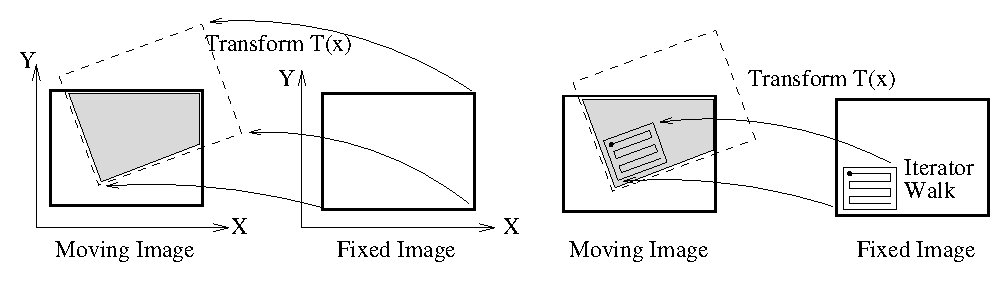
\includegraphics[width=\textwidth]{ImageOverlap.eps}
\itkcaption[Mapping moving image to fixed image in Registration]{ The moving
image is mapped into the fixed image space under some spatial
transformation. An iterator walks through the fixed image and its coordinates
are mapped onto the moving image.}
\label{fig:ImageOverlapIterator}
\end{figure}


\begin{floatingfigure}[rlp]{0.5\textwidth}
 \centering
 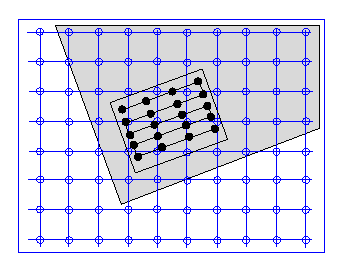
\includegraphics[width=7.5cm]{ImageOverlapInterpolator.eps}
 \caption[Need for interpolation in Registration]{Grid positions of the fixed
image map to non-grid positions of the moving
image.  \label{fig:ImageOverlapInterpolator}}
\end{floatingfigure}

In the registration process, the metric typically compares intensity values
in the fixed image against the corresponding values in the transformed moving
image. When a point is mapped from one space to another by a transform, it
will in general be mapped to a non-grid position. Therefore, interpolation is
required to evaluate the image intensity at the mapped position.

Figure \ref{fig:ImageOverlapIterator} (left) illustrates the mapping of the
fixed image space onto the moving image space. The transform maps points from
the fixed image coordinate system onto the moving image coordinate system. The
figure highlights the region of overlap between the two images after the
mapping. The right side illustrates how an iterator is used to walk through a
region of the fixed image. Each one of the iterator positions is mapped by the
transform onto the moving image space in order to find the homologous pixel.

Figure \ref{fig:ImageOverlapInterpolator} presents a detailed view of the
mapping from the fixed image to the moving image. In general, the grid
positions of the fixed image will not be mapped onto grid positions of the
moving image.  Interpolation is needed for estimating the intensity of the
moving image at these non-grid positions. The service is provided in ITK by
interpolator classes that can be plugged into the registration method.

\index{Nearest\-Neighbor\-Interpolate\-Image\-Function}
\index{Linear\-Interpolate\-Image\-Function}
\index{BSpline\-Interpolate\-Image\-Function}
\index{Windowed\-Sinc\-Interpolate\-Image\-Function}

The following interpolators are available:

\begin{itemize}
\item \doxygen{NearestNeighborInterpolateImageFunction}
\item \doxygen{LinearInterpolateImageFunction}
\item \doxygen{BSplineInterpolateImageFunction}
\item \doxygen{WindowedSincInterpolateImageFunction}
\end{itemize}

In the context of registration, the interpolation method affects the smoothness
of the optimization search space and the overall computation time. On the other
hand, interpolations are executed thousands of times in a single optimization
cycle. Hence, the user has to balance the simplicity of computation with the
smoothness of the optimization when selecting the interpolation scheme.

\index{itk::InterpolateImageFunction}
\index{itk::InterpolateImageFunction!SetInputImage()}
\index{itk::InterpolateImageFunction!Evaluate()}
\index{itk::InterpolateImageFunction!EvaluateAtContinuousIndex()}
\index{itk::InterpolateImageFunction!IsInsideBuffer()}

The basic input to an \doxygen{InterpolateImageFunction} is the image to
be interpolated. Once an image has been defined using \code{SetInputImage()},
a user can interpolate either at a point using \code{Evaluate()} or
an index using \code{EvaluateAtContinuousIndex()}.

Interpolators provide the method \code{IsInsideBuffer()} that tests whether a
particular image index or a physical point falls inside the spatial domain for
which image pixels exist.

\subsection{Nearest Neighbor Interpolation}
\label{sec:NearestNeighborInterpolation}
\index{itk::Nearest\-Neighbor\-Interpolate\-Image\-Function}
The \doxygen{NearestNeighborInterpolateImageFunction} simply uses the
intensity of the nearest grid position. That is, it assumes that the image
intensity is piecewise constant with jumps mid-way between grid positions.
This interpolation scheme is cheap as it does not require any floating point
computations.


\subsection{Linear Interpolation}
\label{sec:LinearInterpolation}
\index{itk::Linear\-Interpolate\-Image\-Function}

The \doxygen{LinearInterpolateImageFunction} assumes that intensity varies
linearly between grid positions. Unlike nearest neighbor interpolation, the
interpolated intensity is spatially continuous. However, the intensity
gradient will be discontinuous at grid positions.


\subsection{B-Spline Interpolation}
\label{sec:BSplineInterpolation}
\index{itk::BSpline\-Interpolate\-Image\-Function}

\begin{figure}
\center
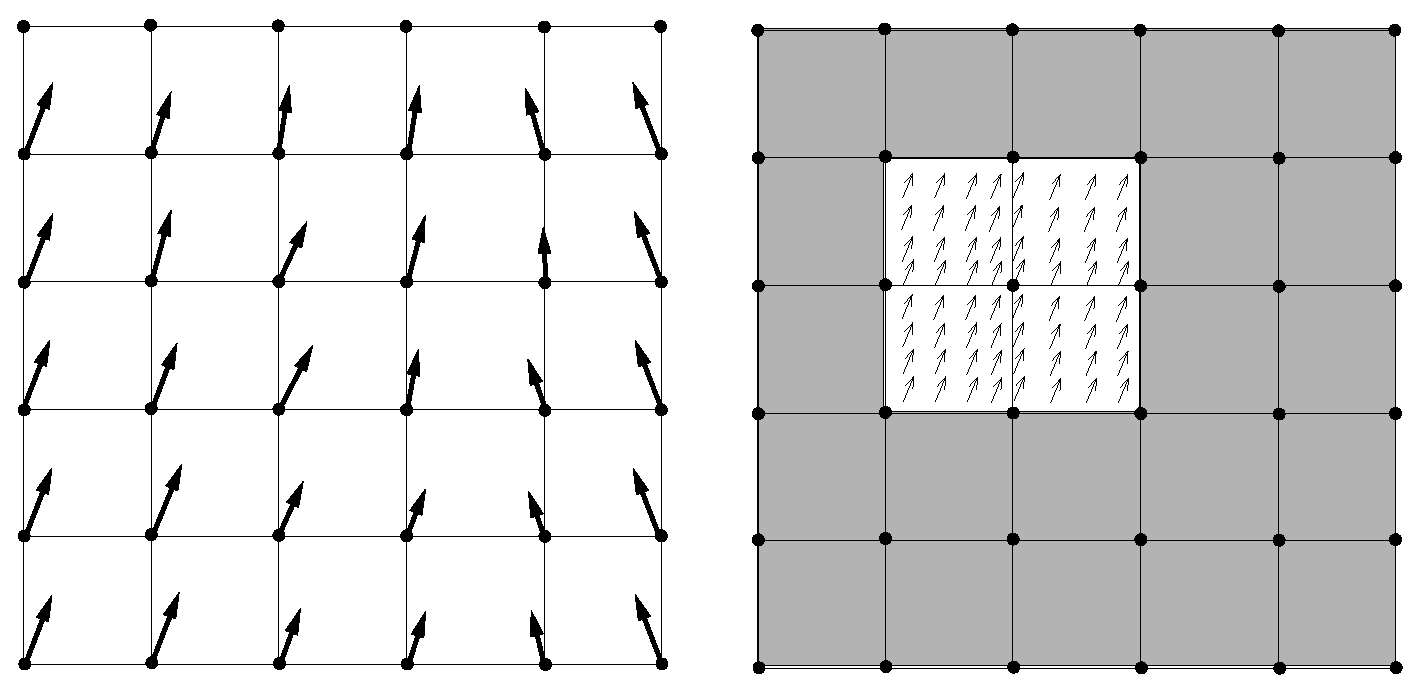
\includegraphics[width=0.9\textwidth]{BSplineInterpolation.eps}
\itkcaption[BSpline Interpolation Concepts]{The left side illustrates the
BSpline grid and the deformations that are known on those nodes. The right side
illustrates the region where interpolation is possible when the BSpline is of
cubic order. The small arrows represent deformation values that were
interpolated from the grid deformations shown on the left side of the diagram.}
\label{fig:BSplineInterpolation}
\end{figure}


The \doxygen{BSplineInterpolateImageFunction} represents the image intensity
using B-spline basis functions. When an input image is first connected to the
interpolator, B-spline coefficients are computed using recursive filtering
(assuming mirror boundary conditions). Intensity at a non-grid position is
computed by multiplying the B-spline coefficients with shifted B-spline kernels
within a small support region of the requested position.
Figure~\ref{fig:BSplineInterpolation} illustrates on the left how the
deformation values on the BSpline grid nodes are used for computing
interpolated deformations in the rest of space. Note for example that when a
cubic BSpline is used, the grid must have one extra node in one side of the
image and two extra nodes on the other side, this along every dimension.

Currently, this interpolator supports splines of order $0$ to $5$. Using a
spline of order $0$ is almost identical to nearest neighbor interpolation; a
spline of order $1$ is exactly identical to linear interpolation. For splines
of order greater than $1$, both the interpolated value and its derivative are
spatially continuous.

It is important to note that when using this scheme, the interpolated
value may lie outside the range of input image intensities. This is
especially important when handling unsigned data, as it is possible
that the interpolated value is negative.


\subsection{Windowed Sinc Interpolation}
\label{sec:WindowedSincInterpolation}
\index{itk::Windowed\-Sinc\-Interpolate\-Image\-Function}

The \doxygen{WindowedSincInterpolateImageFunction} is the best possible
interpolator for data that have been digitized in a discrete grid. This
interpolator has been developed based on Fourier Analysis considerations. It
is well known in signal processing that the process of sampling a spatial
function using a periodic discrete grid results in a replication of the
spectrum of that signal in the frequency domain.

The process of recovering the continuous signal from the discrete sampling is
equivalent to the removal of the replicated spectra in the frequency domain.
This can be done by multiplying the spectra with a box function that will set
to zero all the frequencies above the highest frequency in the original signal.
Multiplying the spectrum with a box function is equivalent to convolving the
spatial discrete signal with a sinc function

\begin{equation}
sinc(x) = \sin{(x)} / x
\end{equation}

The sinc function has infinite support, which of course in practice can not
really be implemented. Therefore, the sinc is usually truncated by multiplying
it with a Window function. The Windowed Sinc interpolator is the result of such an
operation.

This interpolator presents a series of trade-offs in its utilization. Probably
the most significant is that the larger the window, the more precise will be
the resulting interpolation. However, large windows will also result in long
computation times. Since the user can select the window size in this
interpolator, it is up to the user to determine how much interpolation quality
is required in her/his application and how much computation time can be
justified. For details on the signal processing theory behind this
interpolator, please refer to Meijering \emph{et.
al}~\cite{SignalReconstruction}.

The region of the image used for computing the interpolator is determined by
the window \emph{radius}. For example, in a $2D$ image where we want to
interpolate the value at position $(x,y)$ the following computation will be
performed.

\begin{equation}
I(x,y) =
\sum_{i = \lfloor x \rfloor + 1 - m}^{\lfloor x \rfloor + m}
\sum_{j = \lfloor y \rfloor + 1 - m}^{\lfloor y \rfloor + m}
I_{i,j} K(x-i) K(y-j)
\end{equation}

where $m$ is the \emph{radius} of the window. Typically, values such as 3 or 4
are reasonable for the window radius. The function kernel $K(t)$ is composed by
the $sinc$ function and one of the windows listed above.

\begin{equation}
K(t) = w(t) \textrm{sinc}(t) = w(t) \frac{\sin(\pi t)}{\pi t}
\end{equation}

Some of the windows that can be used with this interpolator are

Cosinus window
\begin{equation}
w(x) = cos ( \frac{\pi x}{2 m} )
\end{equation}


Hamming window
\begin{equation}
w(x) = 0.54 + 0.46 cos ( \frac{\pi x}{m} )
\end{equation}


Welch window
\begin{equation}
w(x) = 1 - ( \frac{x^2}{m^2} )
\end{equation}


Lancos window
\begin{equation}
w(x) = \textrm{sinc} ( \frac{x}{m} )
\end{equation}


Blackman window
\begin{equation}
w(x) = 0.42 + 0.5 cos(\frac{\pi x}{m}) + 0.08 cos(\frac{2 \pi x}{m})
\end{equation}


The window functions listed above are available inside the itk::Function
namespace. The conclusions of the referenced paper suggest to use the Welch,
Cosine, Kaiser, and Lancos windows for m = 4,5. These are based on error in
rotating medical images with respect to the linear interpolation method. In
some cases the results achieve a 20-fold improvement in accuracy.

This filter can be used in the same way you would use any
ImageInterpolationFunction. For instance, you can plug it into the
ResampleImageFilter class.  In order to instantiate the filter you must choose
several template parameters.

\small
\begin{minted}[baselinestretch=1,fontsize=\footnotesize,linenos=false,bgcolor=ltgray]{c++}
using InterpolatorType = WindowedSincInterpolateImageFunction<
           TInputImage, VRadius, TWindowFunction,
           TBoundaryCondition, TCoordRep >;

\end{minted}
\normalsize

\code{TInputImage} is the image type, as for any other interpolator.

\code{VRadius} is the radius of the kernel, i.e., the $m$ from the
formula above.

\code{TWindowFunction} is the window function object, which you can choose from
about five different functions defined in this header. The default is the
Hamming window, which is commonly used but not optimal according to the cited
paper.

\code{TBoundaryCondition} is the boundary condition class used to determine the
values of pixels that fall off the image boundary. This class has the same
meaning here as in the \doxygen{NeighborhoodIterator} classes.

\code{TCoordRep} is again standard for interpolating functions, and should be
float or double.


The WindowedSincInterpolateImageFunction is probably not the interpolator that
you want to use for performing registration. Its computation burden makes it
too expensive for this purpose. The best use of this interpolator is for the
final resampling of the image, once the transform has been found using
another less expensive interpolator in the registration process.

\fi

% the clearpage command helps to avoid orphans in the title of the next
% section.
\clearpage

\section{Metrics}
\label{sec:Metrics}
\ifitkFullVersion
%
%  This file is included by Registration.tex
%
%
%

\index{itk::Image\-To\-Image\-Metric}

In ITK, \doxygen{ImageToImageMetric} objects quantitatively measure how well
the transformed moving image fits the fixed image by comparing the gray-scale
intensity of the images. These metrics are very flexible and can work with any
transform or interpolation method and do not require reduction of the
gray-scale images to sparse extracted information such as edges.

The metric component is perhaps the most critical element of the registration
framework. The selection of which metric to use is highly dependent on the
registration problem to be solved. For example, some metrics have a large
capture range while others require initialization close to the optimal
position.  In addition, some metrics are only suitable for comparing images 
obtained from the same imaging modality, while others can handle 
inter-modality comparisons.
Unfortunately, there are no clear-cut rules as to how to choose a metric.

\index{itk::Image\-To\-Image\-Metric!GetValue()}
\index{itk::Image\-To\-Image\-Metric!GetDerivatives()}
\index{itk::Image\-To\-Image\-Metric!GetValueAndDerivatives()}

The basic inputs to a metric are: the fixed and moving images, a transform and
an interpolator. The method \code{GetValue()} can be used to evaluate the
quantitative criterion at the transform parameters specified in the argument.
Typically, the metric samples points within a defined region of the fixed
image.  For each point, the corresponding moving image position is computed
using the transform with the specified parameters, then the interpolator is
used to compute the moving image intensity at the mapped position. Details on
this mapping are illustrated in Figures \ref{fig:ImageOverlapIterator} and
\ref{fig:ImageOverlapInterpolator}. 

The metrics also support region based evaluation. The \code{SetFixedImageMask()} and 
\code{SetMovingImageMask()} methods may be used to restrict evaluation of the metric 
within a specified region. The masks may be of any type derived from \doxygen{SpatialObject}.

Besides the measure value, gradient-based optimization schemes also require
derivatives of the measure with respect to each transform parameter. The
methods \code{GetDerivatives()} and \code{GetValueAndDerivatives()} can be
used to obtain the gradient information.


The following is the list of metrics currently available in ITK:
\begin{itemize}
\item mean squares\\ \doxygen{MeanSquaresImageToImageMetric}
\item normalized correlation \\ \doxygen{NormalizedCorrelationImageToImageMetric}
\item mean reciprocal squared difference \\ \doxygen{MeanReciprocalSquareDifferenceImageToImageMetric} 
\item mutual information by Viola and Wells \\ \doxygen{MutualInformationImageToImageMetric}
\item mutual information by Mattes \\ \doxygen{MattesMutualInformationImageToImageMetric}
\item Kullback Liebler distance metric by Kullback and Liebler \\ \doxygen{KullbackLeiblerCompareHistogramImageToImageMetric}
\item Normalized mutual information \\ \doxygen{NormalizedMutualInformationHistogramImageToImageMetric}
\item Cardinality Match metric \\ \doxygen{MatchCardinalityImageToImageMetric}
\item Kappa Statistics metric\\ \doxygen{KappaStatisticImageToImageMetric}
\item Gradient Difference metric \\ \doxygen{GradientDifferenceImageToImageMetric}
\end{itemize}

In the following sections, we describe each metric type in detail. 
For ease of notation, we will refer to the fixed image $f(\bf{X})$ 
and transformed moving image $(m \circ T(\bf{X}))$ as images $A$ and $B$.

\subsection{Mean Squares Metric}
\label{sec:MeanSquaresMetric}
\index{itk::Mean\-Squares\-Image\-To\-Image\-Metric}

The \doxygen{MeanSquaresImageToImageMetric} computes the mean squared
pixel-wise difference in intensity between image $A$ and $B$ over a user
defined region:

\begin{equation}
MS(A,B) = \frac{1}{N} \sum_{i=1}^N \left( A_i - B_i \right)^2
\end{equation}
\begin{center}
$A_i$ is the i-th pixel of Image A\\ 
$B_i$ is the i-th pixel of Image B\\
$N$ is the number of pixels considered
\end{center}

The optimal value of the metric is zero. Poor matches between images $A$ and
$B$ result in large values of the metric. This metric is simple to compute and
has a relatively large capture radius.

This metric relies on the assumption that intensity representing the same
homologous point must be the same in both images. Hence, its use is restricted
to images of the same modality. Additionally, any linear changes in the
intensity result in a poor match value.

\subsubsection{Exploring a Metric}
\label{sec:ExploringAMetric}

Getting familiar with the characteristics of the Metric as a cost function is
fundamental in order to find the best way of seting up an optimization process
that will use this metric for solving a registration problem. 

\ifitkFullVersion
\input{MeanSquaresImageMetric1.tex}
\fi


\subsection{Normalized Correlation Metric}
\label{sec:NormalizedCorrelationMetric}
\index{itk::Normalized\-Correlation\-Image\-To\-Image\-Metric}

The \doxygen{NormalizedCorrelationImageToImageMetric} computes pixel-wise
cross-correlation and normalizes it by the square root of the autocorrelation
of the images:

\begin{equation}
NC(A,B) = -1 \times \frac{ \sum_{i=1}^N \left( A_i \cdot B_i \right) }
        { \sqrt { \sum_{i=1}^N A_i^2  \cdot \sum_{i=1}^N B_i^2 } }
\end{equation}
\begin{center}
$A_i$ is the i-th pixel of Image A\\ 
$B_i$ is the i-th pixel of Image B\\
$N$ is the number of pixels considered
\end{center}

Note the $-1$ factor in the metric computation. This factor is used to make the
metric be optimal when its minimum is reached.  The optimal value of the metric
is then minus one. Misalignment between the images results in small measure
values.  The use of this metric is limited to images obtained using the same
imaging modality.  The metric is insensitive to multiplicative factors between
the two images.  This metric produces a cost function with sharp peaks and well
defined minima.  On the other hand, it has a relatively small capture radius.

\subsection{Mean Reciprocal Square Differences}
\label{sec:MeanReciprocalSquareDifferenceMetric}
\index{itk::Mean\-Reciprocal\-Square\-Difference\-Image\-To\-Image\-Metric}

The \doxygen{MeanReciprocalSquareDifferenceImageToImageMetric} computes
pixel-wise differences and adds them after passing them through a bell-shaped
function $\frac{1}{1+x^2}$:

\begin{equation}
PI(A,B) =  \sum_{i=1}^N \frac{ 1 }{ 1 + \frac{ \left( A_i - B_i \right) ^ 2}{ \lambda^2 }  }
\end{equation}
\begin{center}
$A_i$ is the i-th pixel of Image A \\
$B_i$ is the i-th pixel of Image B \\
$N$ is the number of pixels considered \\
$\lambda$ controls the capture radius
\end{center}

The optimal value is $N$ and poor matches results in small measure values.
The characteristics of this metric have been studied by Penney and Holden
\cite{Holden1999}\cite{Penney1998}

This image metric has the advantage of producing poor values when few pixels
are considered.  This makes it consistent when its computation is subject to
the size of the overlap region between the images. The capture radius of the
metric can be regulated with the parameter $\lambda$.  The profile of this
metric is very peaky. The sharp peaks of the metric help to measure spatial
misalignment with high precision. Note that the notion of capture radius is
used here in terms of the intensity domain, not the spatial domain. In that
regard, $\lambda$ should be given in intensity units and be associated with
the differences in intensity that will make drop the metric by $50\%$.

The metric is limited to images of the same image modality.  The
fact that its derivative is large at the central peak is a problem for some
optimizers that rely on the derivative to decrease as the extrema are
reached.  This metric is also sensitive to linear changes in intensity.


\subsection{Mutual Information Metric}
\label{sec:MutualInformationMetric}

The \doxygen{MutualInformationImageToImageMetric} computes the mutual
information between image $A$ and image $B$.  Mutual information (MI)
measures how much information one random variable (image intensity in one
image) tells about another random variable (image intensity in the other
image). The major advantage of using MI is that the actual form of the
dependency does not have to be specified.  Therefore, complex mapping between
two images can be modeled.  This flexibility makes MI well suited as a
criterion of multi-modality registration~\cite{Pluim2003}.

Mutual information is defined in terms of entropy. Let
\begin{equation}
H(A) = - \int p_A(a) \log p_A(a)\, da
\end{equation}
be the entropy of random variable $A$, $H(B)$ the entropy of 
random variable $B$ and 
\begin{equation}
H(A,B) = \int p_{AB}(a,b) \log p_{AB}(a,b)\,da\,db
\end{equation}
be the joint entropy of $A$ and $B$. If $A$ and $B$ are independent, then
\begin{equation}
p_{AB}(a,b) = p_A(a) p_B(b)
\end{equation}
and
\begin{equation}
H(A,B) = H(A) + H(B).
\end{equation}
However, if there is any dependency, then
\begin{equation}
H(A,B)<H(A)+H(B).
\end{equation}
The difference is called Mutual Information : \( I(A,B) \)
\begin{equation}
I(A,B)=H(A)+H(B)-H(A,B)
\end{equation}

\subsubsection{Parzen Windowing}

\itkpiccaption[Parzen Windowing in Mutual Information]{
In Parzen windowing, a continuous density function is constructed by
superimposing kernel functions (Gaussian function in this case) centered on the
intensity samples obtained from the image.\label{fig:ParzenWindowing}}
\parpic(0.5\textwidth,5.5cm)[r]{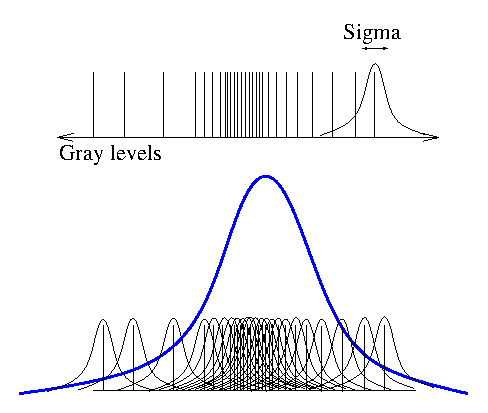
\includegraphics[width=0.48\textwidth]{ParzenWindowing13.eps}}

In a typical registration problem, direct access to the marginal 
and joint probability densities is not available and hence the
densities must be estimated from the image data. Parzen windows 
(also known as kernel density estimators) can be used for this purpose.
In this scheme, the densities are constructed by taking intensity 
samples $S$ from the image and super-positioning kernel functions 
$K(\cdot)$ centered on the elements of $S$ as illustrated in
Figure \ref{fig:ParzenWindowing}:

A variety of functions can be used as the smoothing kernel with the
requirement that they are smooth, symmetric, have zero mean and
integrate to one. For example, boxcar, Gaussian and B-spline functions are
suitable candidates.  A smoothing parameter is used to scale the kernel
function.  The larger the smoothing parameter, the wider the kernel function
used and hence the smoother the density estimate. If the parameter is too
large, features such as modes in the density will get smoothed out.  On the
other hand, if the smoothing parameter is too small, the resulting density
may be too noisy. The estimation is given by the following equation.

\begin{equation}
p(a) \approx P^{*}(a) = \frac{1}{N} \sum_{s_j \in S} K\left(a - s_j\right)
\end{equation}

Choosing the optimal smoothing parameter is a difficult research problem and
beyond the scope of this software guide.  Typically, the optimal value of the
smoothing parameter will depend on the data and the number of samples used.

\subsubsection{Viola and Wells Implementation}

The Insight Toolkit has two mutual information metric implementations. The
first is \doxygen{MutualInformationImageToImageMetric} and follows the method
specified by Viola and Wells in \cite{Viola1997}.

\index{itk::Mutual\-Information\-Image\-To\-Image\-Metric}

In this implementation, two separate intensity samples $S$ and $R$ are drawn
from the image: the first to compute the density, and the second to approximate
the entropy as a sample mean:
\begin{equation}
H(A) = \frac{1}{N} \sum_{r_j \in R} \log P^{*}(r_j).
\end{equation}
Gaussian density is used as a smoothing kernel, where the standard deviation
$\sigma$ acts as the smoothing parameter.

\index{itk::Mutual\-Information\-Image\-To\-Image\-Metric!SetNumberOfSpatialSamples()}

The number of spatial samples used for computation is defined using
the \code{SetNumberOfSpatialSamples()} method. Typical values range from 50 to 100.
Note that computation involves an $N \times N$ loop and hence, the computation
burden becomes very expensive when a large number of samples is used.

\index{itk::Mutual\-Information\-Image\-To\-Image\-Metric!SetFixedImageStandardDeviation()}
\index{itk::Mutual\-Information\-Image\-To\-Image\-Metric!SetMovingImageStandardDeviation()}
The quality of the density estimates depends on the choice of the standard
deviation of the Gaussian kernel. The optimal choice will depend on the
content of the images.  In our experience with the toolkit, we have found
that a standard deviation of 0.4 works well for images that have been
normalized to have a mean of zero and standard deviation of 1.0. The standard
deviation of the fixed image and moving image kernel can be set separately
using methods
\code{SetFixedImageStandardDeviation()} and \code{SetMovingImageStandardDeviation()}.

\subsubsection{Mattes et al. Implementation}
The second form of mutual information metric available in ITK follows the
method specified by Mattes et al. in \cite{Mattes2001} and is implemented by
the \doxygen{MattesMutualInformationImageToImageMetric} class.

\index{itk::Mattes\-Mutual\-Information\-Image\-To\-Image\-Metric}
In this implementation, only one set of intensity samples is drawn from the
image.  Using this set, the marginal and joint probability density function
(PDF) is evaluated at discrete positions or bins uniformly spread within the
dynamic range of the images. Entropy values are then computed by summing over
the bins.

\index{itk::Mattes\-Mutual\-Information\-Image\-To\-Image\-Metric!SetNumberOfSpatialSamples()}
\index{itk::Mattes\-Mutual\-Information\-Image\-To\-Image\-Metric!SetNumberOfHistogramBins()}

The number of spatial samples used is set using method 
\code{SetNumberOfSpatialSamples()}. The number of bins used to compute
the entropy values is set via \code{SetNumberOfHistogramBins()}.

Since the fixed image PDF does not contribute to the metric derivatives, it
does not need to be smooth. Hence, a zero order (boxcar) B-spline kernel is
used for computing the PDF. On the other hand, to ensure smoothness, a third
order B-spline kernel is used to compute the moving image intensity PDF. The
advantage of using a B-spline kernel over a Gaussian kernel is that the
B-spline kernel has a finite support region. This is computationally
attractive, as each intensity sample only affects a small number of bins and
hence does not require a $N \times N$ loop to compute the metric value.

During the PDF calculations, the image intensity values are linearly scaled
to have a minimum of zero and maximum of one. This rescaling means that a
fixed B-spline kernel bandwidth of one can be used to handle image data with
arbitrary magnitude and dynamic range.


\subsection{Kullback-Leibler distance metric}
Another information based metric is the \doxygen{KullbackLeiblerCompareHistogramImageToImageMetric} metric. Kullback-Leibler distance measures the relative entropy between two discrete 
probability distributions. The distributions are obtained from the histograms of the two 
input images, $A$ and $B$. 

The Kullback-Liebler distance between two histograms is given by
\begin{equation}
KL(A,B) =  \sum_i^N p_A(i) \times \log \frac{ p_A(i) }{p_B(i) }
\end{equation}

The distance is always non-negative and is zero only if the two distributions 
are the same. Note that the distance is not symmetric. In other 
words, $KL(A,B) \neq KL(B,A)$. Nevertheless, if the distributions are not too dissimilar, 
the difference betwween $KL(A,B)$ and $KL(B,A)$ is small.

The implementation in ITK is based on \cite{Chung2002}

\subsection{Normalized Mutual Information Metric}
Given two images, $A$ and $B$, the normalized mutual information may be computed as 
\begin{equation}
NMI(A,B) = 1 + \frac{I(A,B)}{H(A,B)} = \frac{H(A) + H(B)}{H(A,B)}
\end{equation}
where the entropy of the images, $H(A)$, $H(B)$, the mutual 
inoformation, $I(A,B)$ and the joint entropy $H(A,B)$ are computed as mentioned 
in \ref{sec:MutualInformationMetric}. Details of the implementation may be found in 
the \cite{Hajnal2001}.

\subsection{Cardinality Match Metric}
\index{itk::Match\-Cardinality\-Image\-To\-Image\-Metric}
The \doxygen{MatchCardinalityImageToImageMetric} computes cardinality of the set of pixels 
that match exactly between the moving and fixed images. In other words, it computes the 
number of pixel matches and mismatches between the two images. The match is designed for 
label maps. All pixel mismatches are considered equal whether they are between label 1 
and label 2 or between label 1 and label 500. In other words, the magnitude of an 
individual label mismatch is not relevant, or the occurence of a label mismatch 
is important. 

The spatial correspondance between the fixed and moving images is established using 
a \doxygen{Transform} using the \code{SetTransform()} method and an interpolator 
using \code{SetInterpolator()}. Given that we are matching pixels with labels, 
it is advisable to use Nearest Neighbor interpolation.

\subsection{Kappa Statistics Metric}
\index{itk::Kappa\-Statistic\-Image\-To\-Image\-Metric}
The \doxygen{KappaStatisticImageToImageMetric} computes spatial intersection of 
two binary images. The metric here is designed for matching pixels in two images 
with the same exact value, which may be set using \code{SetForegroundValue()}. 
Given two images $A$ and $B$, the $\kappa$ coefficient is computed as
 
\begin{equation}
\kappa = \frac{|A| \cap |B|}{|A| + |B|}
\end{equation}

This computes the fraction of area in the two images that is common to both 
the images. In the computation of the metric, only foreground pixels are considered.

\subsection{Gradient Difference Metric}
\index{it::Gradient\-Difference\-Image\-To\-Image\-Metric}
This \doxygen{GradientDifferenceImageToImageMetric} metric evaluates the 
difference in the derivatives of the moving and fixed images. and adds 
them after passing them through a function $\frac{1}{1+x}$.



\fi

% the clearpage command helps to avoid orphans in the title of the next
% section.
\clearpage

\section{Optimizers}
\label{sec:Optimizers}
\ifitkFullVersion

\index{itk::Optimizer|textbf}
\index{itk::SingleValuedNonLinearOptimizer|textbf}


\begin{figure}
\center
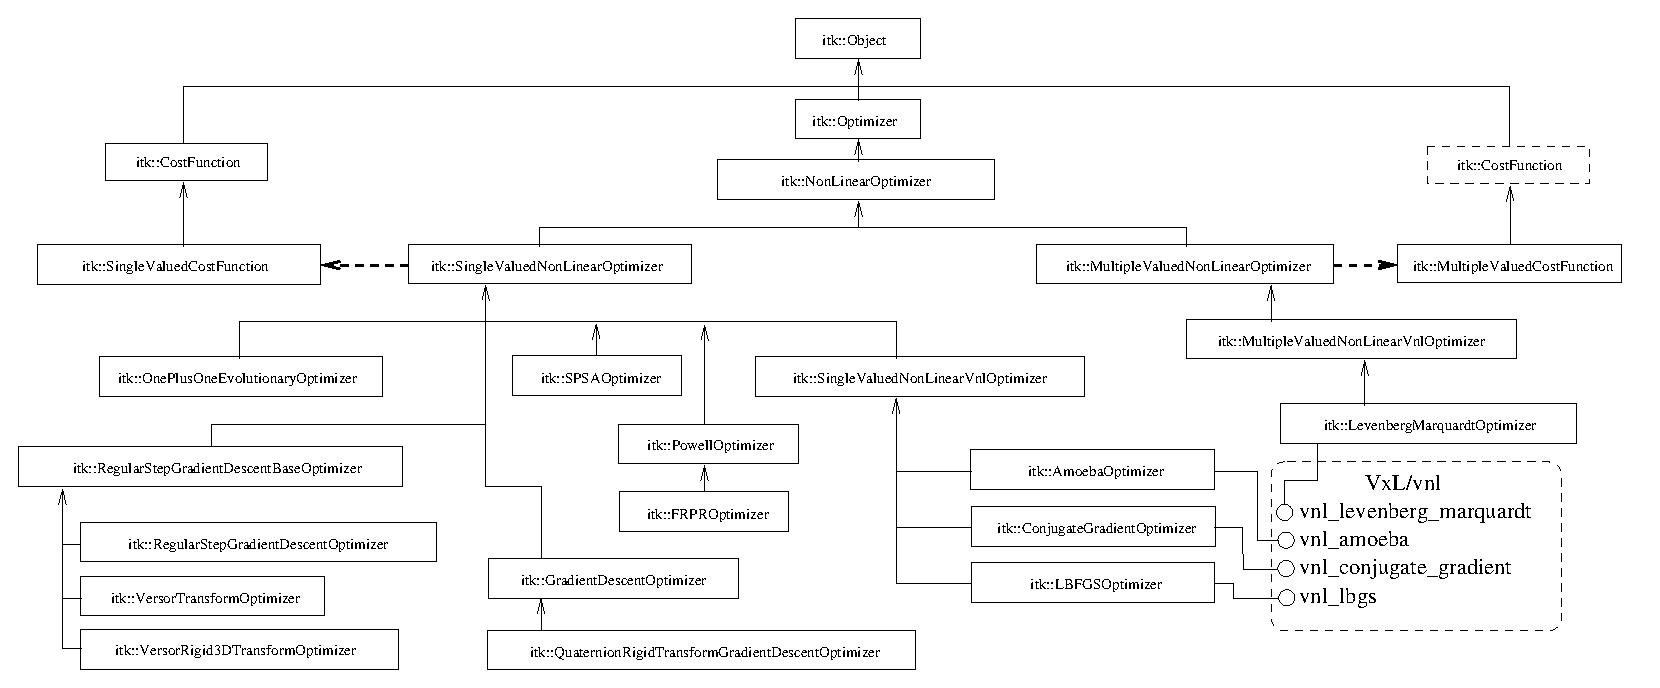
\includegraphics[width=16cm]{OptimizersHierarchy.eps}
\itkcaption{Class diagram of the Optimizers hierarchy.}
\label{fig:OptimizersHierarchy}
\end{figure}

Optimization algorithms are encapsulated as \code{itk::Optimizer} objects
within ITK. Optimizers are generic and can be used for applications other than
registration.  Within the registration framework,
\code{itk::SingleValuedNonLinearOptimizer} are used to optimize the metric
criterion with respect to the transform parameters.

\index{itk::Optimizer!SetInitialPosition()}
\index{itk::Optimizer!StartOptimization()}
\index{itk::Optimizer!GetCurrentPosition()}

The basic input to an optimizer is a cost function object. In the context
of registration, \code{itk::ImageToImageMetric} provide this functionality.
The initial parameters are set using \code{SetInitialPosition()} and
the optimization algorithm is invoked by \code{StartOptimization()}.
Once the optimization has finished, the final parameters can be obtained
using \code{GetCurrentPosition()}.

\index{itk::Optimizer!SetScales()}
Some optimizers also allows rescaling of the individual parameters. This
is convenient for normalizing parameters spaces where some parameters
have different dynamic ranges. For example, the first parameter of
\code{Euler2DTransform} represent an angle while the last two parameters
the translation. A unit change in angle has a much greater impact on
an image than a unit change in translation. This difference in scale appears
as long narrow valleys in the search space making the optimization problem
diffcult. Rescaling the translation parameters can help to fix this problem.
Scales are represented as \code{Array} of doubles and set defined using
\code{SetScales()}.

The types of \code{itk::SingleValuedNonLinearOptimizer} currently available
in ITK are:

\index{itk::AmoebOptimizer|textbf}
\index{itk::ConjugateGradientOptimizer|textbf}
\index{itk::GradientDescentOptimizer|textbf}
\index{itk::QuaternionRigidTransformGradientDescentOptimizer|textbf}
\index{itk::LBFGSOptimizer|textbf}
\index{itk::OnePlusOneEvolutionaryOptimizer|textbf}
\index{itk::RegularStepGradientDescentOptimizer|textbf}
\index{itk::VersorTransformOptimizer|textbf}
\index{itk::LevenbergMarquardtOptimizer|textbf}

\begin{itemize}

\item \textbf{Amoeba}: Nelder-Meade downhill simplex.  This optimizer is
actually implemented in the \code{VxL/vnl} numerics toolkit.  The ITK class
\code{itk::AmoebaOptimizer} is merely an adaptor class.

\item \textbf{Conjugate Gradient}: Fletcher-Reeves form 
of conjugate gradient with or without preconditioning. Also an adaptor to an
optimizer in \code{vnl}.

\item \textbf{Gradient Descent}: Advance parameters in the direction of the
gradient where the step size is governed by a learning rate. 

\item \textbf{Quaternion Rigid Transform Gradient Descent}: 
A specialized version of \code{GradientDescentOptimizer} for
\code{QuaternionRigidTransform} parameters, where the parameters representing
the quaternion is normalize to a magnitude to one at each iteration to
represent a pure rotation.

\item \textbf{LBFGS}: Limited memory Broyden, Fletcher, Goldfarb
and Shannon minmization. It is an adaptor to an optimizer in \code{vnl}.

\item \textbf{One Plus One Evolutionary}: Strategy that simulates the
biological evolution of a set of samples in the search space. This optimizer
is mainly used in the process of bias correction for MRI images.

\item \textbf{Regular Step Gradient Descent}: Advance parameters in the
direction of the gradient where a bipartition scheme is used to compute
the step size. 

\item \textbf{Versor Transform Optimizer}: A specialized version of
\code{RegularStepGradientDescentOptimizer} for \code{VersorTransform}
parameters  where the current rotation is composed with the gradient rotation
to produce the new rotation vector. It follows the definition of versor
gradients defined by Hamilton~\cite{Hamilton1866}.

\end{itemize}

A parallel hierarchy exists for optimizing multiple-valued cost functions. The
base optimizer in this branch of the hierarchy is the
\code{itk::MultipleValuedNonLinearOptimizer} whose only current derived class
is:

\begin{itemize}

\item \textbf{Levenberg Marquardt}: Non-linear least squares minimization.
Adapted to an optimizer in \code{vnl}.

\end{itemize}


Figure \ref{fig:OptimizersHierarchy} illustrates the full class hierarchy of
optimizers in ITK. Optimizers in the lower right corner are adaptors classes to
optimizers existing in the \code{VxL/vnl} numerics toolkit. The optimizers
interact with the \code{itk::CostFunction} class. In the registration framework
this cost function is reimplemented in the form of \code{itk::ImageToImageMetric}.






\fi



\subsection{Registration using Match Cardinality metric}
\label{sec:RegistrationMatchCardinality}
\ifitkFullVersion
\input{ImageRegistration10.tex}
\fi


\subsection{Registration using the One plus One Evolutionary Optimizer}
\label{sec:RegistrationOnePlusOne}
\ifitkFullVersion
\input{ImageRegistration11.tex}
\fi



\subsection{Registration using masks constructed with Spatial objects}
\label{sec:RegistrationSpatialObjects}
\ifitkFullVersion
\input{ImageRegistration12.tex}
\fi



\subsection{Rigid registrations incorporating prior knowledge}
\label{sec:RegistrationCentered2DTransform}
\ifitkFullVersion
\input{ImageRegistration13.tex}
\fi


% the clearpage command helps to avoid orphans in the title of the next
% section.
\clearpage


\section{Image Pyramids}
\label{sec:ImagePyramids}
\ifitkFullVersion

\index{itk::Multi\-Resolution\-Pyramid\-Image\-Filter}

In ITK, the \doxygen{MultiResolutionPyramidImageFilter} can be used to create
a sequence of reduced resolution images from the input image.  The
down-sampling is performed according to a user defined multi-resolution
schedule. The schedule is specified as an \doxygen{Array2D} of integers,
containing shrink factors for each multi-resolution level (rows) for each
dimension (columns). For example,

\small
\begin{verbatim}
8 4 4
4 4 2
\end{verbatim}
\normalsize

is a schedule for a three dimensional image for two multi-resolution levels.
In the first (coarsest) level, the image is reduced by a factor of 8
in the column dimension, factor of 4 in the row dimension and a factor
of 4 in the slice dimension. In the second level, the image reduced
by a factor of 4 in the column dimension, 4 in the row dimension and
2 in the slice dimension.

\index{itk::Multi\-Resolution\-Pyramid\-Image\-Filter!SetNumberOfLevels()}

The method \code{SetNumberOfLevels()} is used to set the number of
resolution levels in the pyramid. This method will allocate memory
for the schedule and generate a default table with the starting
(coarsest) shrink factors for all dimensions set to $2^(M-1)$,
where $M$ is the number of levels. All factors are halved for
all subsequent levels. For example, if we set the number of levels
to 4, the default schedule is then:

\small
\begin{verbatim}
8 8 8
4 4 4
2 2 2
1 1 1
\end{verbatim}
\normalsize

\index{itk::Multi\-Resolution\-Pyramid\-Image\-Filter!GetSchedule()}
\index{itk::Multi\-Resolution\-Pyramid\-Image\-Filter!SetSchedule()}
\index{itk::Multi\-Resolution\-Pyramid\-Image\-Filter!SetStartingShrinkFactors()}

The user can get a copy of the schedule using method \code{GetSchedule()},
make modifications, and reset it using method \code{SetSchedule()}.
Alternatively, a user can create a default table by specifying the
starting (coarsest) shrink factors using the method
\code{SetStartingShrinkFactors()}. The factors for the subsequent
levels are generated by halving the factor or setting it to one,
depending on which is larger. For example, for a 4 level pyramid
and starting factors of 8, 8 and 4, the generated schedule would be:

\small
\begin{verbatim}
8 8 4
4 4 2
2 2 1
1 1 1
\end{verbatim}
\normalsize

When this filter is triggered by \code{Update()}, $M$ outputs are produced
where the $m$-th output corresponds to the $m$-th level of the pyramid.
To generate these images, Gaussian smoothing is first performed using a
\doxygen{DiscreteGaussianImageFilter} with the variance set to $(s/2)^2$,
where $s$ is the shrink factor. The smoothed images are then sub-sampled using
a \doxygen{ShrinkImageFilter}.

\fi


% the clearpage command helps to avoid orphans in the title of the next
% section.
\clearpage

\section{Deformable Registration}
\label{sec:DeformableRegistration}
\ifitkFullVersion
%%%%%%%%%%%%%%%%%%%%%%%%%%%%%%%%%%%%%%%%%%%%%%%%%%%%%%%%%%%%%%%
%
%
%   This file is included in Registration.tex
%
%   Labels and section entries are defined in that file.
%
%
%
%%%%%%%%%%%%%%%%%%%%%%%%%%%%%%%%%%%%%%%%%%%%%%%%%%%%%%%%%%%%%%%


\subsection{FEM-Based Image Registration}
\label{sec:FEMBasedImageRegistration}

\begin{figure}
\centering
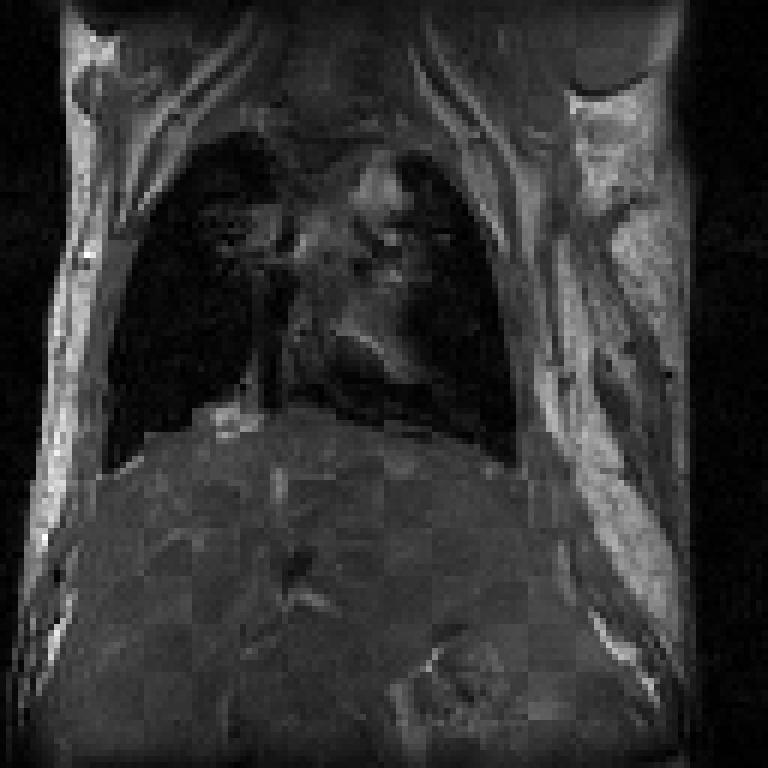
\includegraphics[width=0.44\textwidth]{DeformableRegistration1CheckerboardBefore.eps}
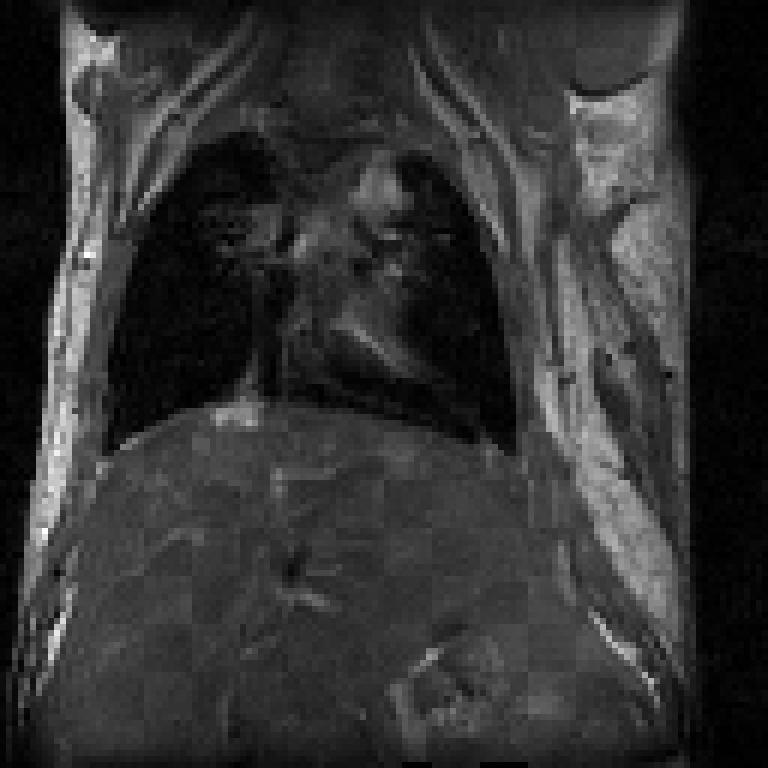
\includegraphics[width=0.44\textwidth]{DeformableRegistration1CheckerboardAfter.eps}
\itkcaption[FEM-based deformable registration results]{Checkerboard comparisons
before and after FEM-based deformable registration.}
\label{fig:DeformableRegistration1Output}
\end{figure}

\input{DeformableRegistration1.tex}

Figure \ref{fig:DeformableRegistration1Output} presents the results of
the FEM-based deformable registration applied to two time-separated
slices of a living rat dataset.  Checkerboard comparisons of the two
images are shown before registration (left) and after registration
(right).  Both images were acquired from the same living rat, the
first after inspiration of air into the lungs and the second after
exhalation.  Deformation occurs due to the relaxation of the diaphragm
and the intercostal muscles, both of which exert force on the lung tissue
and cause air to be expelled.

The following is a documented sample parameter file that can be used with this
deformable registration example.  This example demonstrates the setup of a
basic registration problem that does not use multi-resolution strategies.  As a
result, only one value for the parameters between \texttt{(\# of pixels per
element)} and \texttt{(maximum iterations)} is necessary.  In order to use a
multi-resolution strategy, you would have to specify values for those
parameters at each level of the pyramid.

\small
\verbatiminput{FiniteElementRegistrationParameters1.txt}
\normalsize

\subsection{BSplines Image Registration}
\label{sec:BSplinesImageRegistration}
\input{DeformableRegistration4.tex}


\subsection{Level Set Motion for Deformable Registration}
\label{sec:LevelSetMotionForDeformableRegistration}
\input{DeformableRegistration5.tex}


\subsection{BSplines Multi-Grid Image Registration}
\label{sec:BSplinesMultiGridImageRegistration}
\input{DeformableRegistration6.tex}


\subsection{BSplines Multi-Grid Image Registration in 3D}
\label{sec:BSplinesMultiGridImageRegistrationIn3D}
\input{DeformableRegistration7.tex}


\subsection{Image Warping with Kernel Splines}
\label{sec:ImageWarpingWithKernelSplines}
\input{LandmarkWarping2.tex}


\subsection{Image Warping with BSplines}
\label{sec:ImageWarpingWithBSplines}
\input{BSplineWarping1.tex}

\fi

% the clearpage command helps to avoid orphans in the title of the next
% section.
\clearpage

\section{Demons Deformable Registration}
\label{sec:DemonsDeformableRegistration}
\ifitkFullVersion
%%%%%%%%%%%%%%%%%%%%%%%%%%%%%%%%%%%%%%%%%%%%%%%%%%%%%%%%%%%%%%%
%
%
%   This file is included in Registration.tex
%
%   Lablels and section entries are defined in that file.
%
%
%
%%%%%%%%%%%%%%%%%%%%%%%%%%%%%%%%%%%%%%%%%%%%%%%%%%%%%%%%%%%%%%%

For the problem of intra-modality deformable registration, the Insight
Toolkit provides an implementation of Thirion's ``demons'' algorithm
\cite{Thirion1995b,Thirion1998}. 
In this implementation, each image is viewed as a set of iso-intensity
contours.  The main idea is that a regular grid of forces deform an image by
pushing the contours in the normal direction.  The orientation and magnitude
of the displacement is derived from the instantaneous optical flow equation:

\begin{equation}
\bf{D}(\bf{X}) \cdot \nabla f(\bf{X}) = - \left(m(\bf{X}) - f(\bf{X}) \right)
\label{eqn:OpticalFlow}
\end{equation}

In the above equation, $f(\bf{X})$ is the fixed image, $m(\bf{X})$
is the moving image to be registered, and $\bf{D}(\bf{X})$ is the displacement 
or optical flow between the images. It is well known in optical flow
literature that Equation \ref{eqn:OpticalFlow} is insufficient to specify 
$\bf{D}(\bf{X})$ locally and is usually determined using some form of
regularization. For registration, the projection of the vector on the
direction of the intensity gradient is used:

\begin{equation}
\bf{D}(\bf{X}) = - \frac
{\left(  m(\bf{X}) - f(\bf{X}) \right) \nabla f(\bf{X})}
{\left\|  \nabla f \right\|^2 } 
\end{equation}

However, this equation becomes unstable for small values of the image gradient,
resulting in large displacement values. To overcome this problem, Thirion
re-normalizes the equation such that:

\begin{equation}
\bf{D}(\bf{X}) = - \frac
{\left(  m(\bf{X}) - f(\bf{X}) \right) \nabla f(\bf{X})}
{\left\|  \nabla f \right\|^2 + \left(  m(\bf{X}) - f(\bf{X}) \right)^2 / K } 
\label{eqn:DemonsDisplacement}
\end{equation}

Where $K$ is a normalization factor that accounts for the units imbalance
between intensities and gradients. This factor is computed as the mean squared
value of the pixel spacings. The inclusion of $K$ make the force computation to
be invariant to the pixel scaling of the images.

Starting with an initial deformatin field $\bf{D}^{0}(\bf{X})$, the demons
algorithm iteratively updates the field using Equation
\ref{eqn:DemonsDisplacement} such that the field at the $N$-th iteration is
given by:

\begin{equation}
\bf{D}^{N}(\bf{X}) = \bf{D}^{N-1}(\bf{X}) - \frac
{\left(  m(\bf{X}+ \bf{D}^{N-1}(\bf{X})) 
- f(\bf{X}) \right) \nabla f(\bf{X})}
{\left\|  \nabla f \right\|^2 + \left(  
m(\bf{X}+ \bf{D}^{N-1}(\bf{X}) )
 - f(\bf{X}) \right)^2 } 
\label{eqn:DemonsUpdateEquation}
\end{equation}

Reconstruction of the deformation field is an ill-posed problem where
matching the fixed and moving images has many solutions. For example, since
each image pixel is free to move independently, it is possible that all
pixels of one particular value in $m(\bf{X})$ could map to a single image
pixel in $f(\bf{X})$ of the same value. The resulting deformation field may
be unrealistic for real-world applications. An option to solve for the field
uniquely is to enforce an elastic-like behavior, smoothing the deformation
field with a Gaussian filter between iterations.

In ITK, the demons algorithm is implemented as part of the finite difference
solver (FDS) framework and its use is demonstrated in the following example.

\input{DeformableRegistration2.tex} 

A variant of the force computation is also implemented in which the gradient of
the deformed moving image is also involved. This provides a level of symmetry
in the force calculation during one iteration of the PDE update. The equation
used in this case is

\begin{equation}
\bf{D}(\bf{X}) = - \frac
{2 \left(  m(\bf{X}) - f(\bf{X}) \right) \left(  \nabla f(\bf{X}) +  \nabla g(\bf{X}) \right) }
{\left\|  \nabla f + \nabla g \right\|^2 + \left(  m(\bf{X}) - f(\bf{X}) \right)^2 / K } 
\label{eqn:DemonsDisplacement}
\end{equation}

The following example illustrates the use of this defomable registration
method.

\input{DeformableRegistration3.tex} 




\fi

\section{Visualizing Deformation fields}
\label{sec:VisualizingDeformationFields}
\ifitkFullVersion
%%%%%%%%%%%%%%%%%%%%%%%%%%%%%%%%%%%%%%%%%%%%%%%%%%%%%%%%%%%%%%%
%
%
%   This file is included in Registration.tex
%
%   Lablels and section entries are defined in that file.
%
%
%
%%%%%%%%%%%%%%%%%%%%%%%%%%%%%%%%%%%%%%%%%%%%%%%%%%%%%%%%%%%%%%
Vector deformation fields may be visualized using Paraview.
Paraview \cite{ParaviewBook} is an open-source, multi-platform visualization application and uses the Visualization Toolkit as the data processing and rendering engine and has a user interface written using a unique blend of Tcl/Tk and C++. You may download it from http://paraview.org.

\subsection{Visualizing 2D deformation fields}
Let us visualize the deformation field obtained from Demons Registration algorithm generated from Insight/Examples/Registration/DeformableRegistration2.cxx.

Load the Deformation field in Paraview. (The deformation field must be capable of handling vector data, such as MetaImages). Paraview shows a color map of the magnitudes of the deformation fields as shown in \ref{fig:ParaviewScreenshot1}.

Covert the deformation field to 3D vector data using a {\it Calculator}. The Calculator may be found in the {\it Filter} pull dowm menu. A screenshot of the calculator tab is shown in Figure \ref{fig:ParaviewScreenshot2}. Although the deformation field is a 2D vector, we will generate a 3D vector with the third component set to 0 since Paraview generates glyphs only for 3D vectors. You may now apply a glyph of arrows to the resulting 3D vector field by using {\it Glyph} on the menu bar. The glphs obtained will be very dense since a glyph is generated for each point in the data set. To better visualize the deformation field, you may adopt one of the following approaches. 

Reduce the number of glyphs by reducing the number in {\it Max. Number of Glyphs} to reasonable amount. This uniformly downsamples the number of glyphs. Alternatively, you may apply a {\it Threshold} filter to the {\it Magnitude} of the vector dataset and then glyph the vector data that lies above the threshold. This eliminates the smaller deformation fields that clutter the display. You may now reduce the number of glyphs to a reasonable value.

Figure \ref{fig:ParaviewScreenshot3} shows the vector field visualized using Paraview by thresholding the vector magnitudes by 2.1 and restricting the number of glyphs to 100.

\begin{figure}
\center
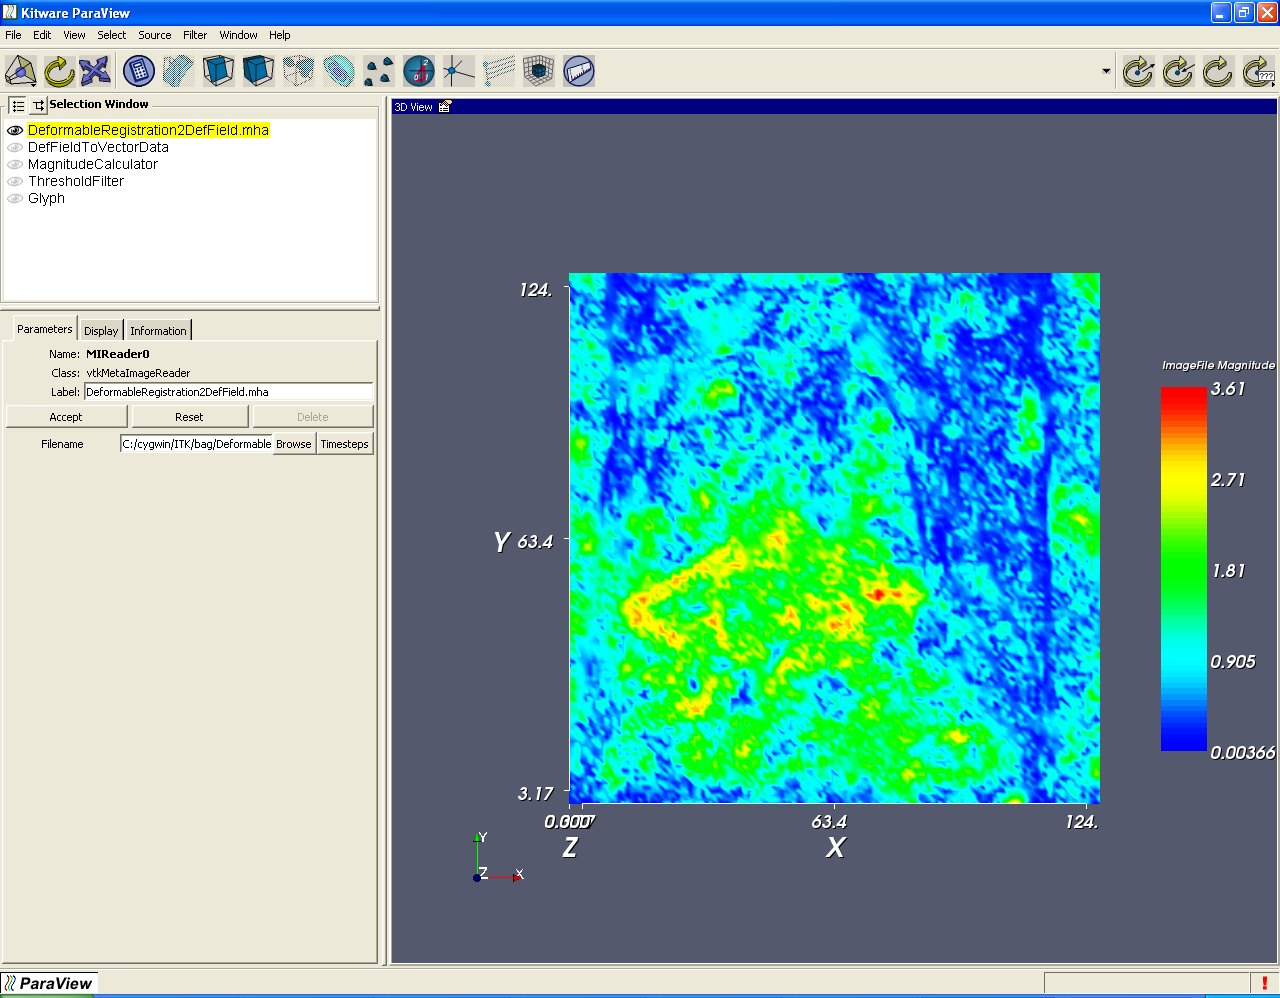
\includegraphics[width=\textwidth]{ParaviewScreenshot1.eps}
\itkcaption[Deformation field magnitudes]{Deformation field magnitudes displayed using Paraview}
\label{fig:ParaviewScreenshot1}
\end{figure}

\begin{figure}
\center
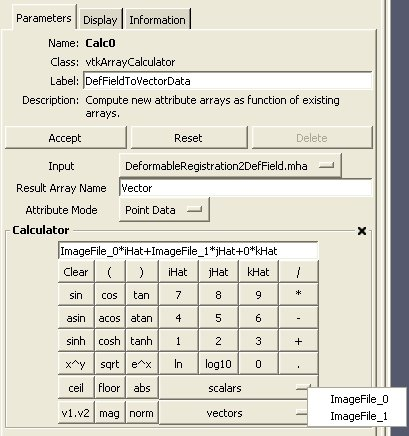
\includegraphics[width=0.3\textwidth]{ParaviewScreenshot2.eps}
\itkcaption[Calculator]{Calculators and filters may be used to compute the vector magnitude, compose vectors etc.}
\label{fig:ParaviewScreenshot2}
\end{figure}

\begin{figure}
\center
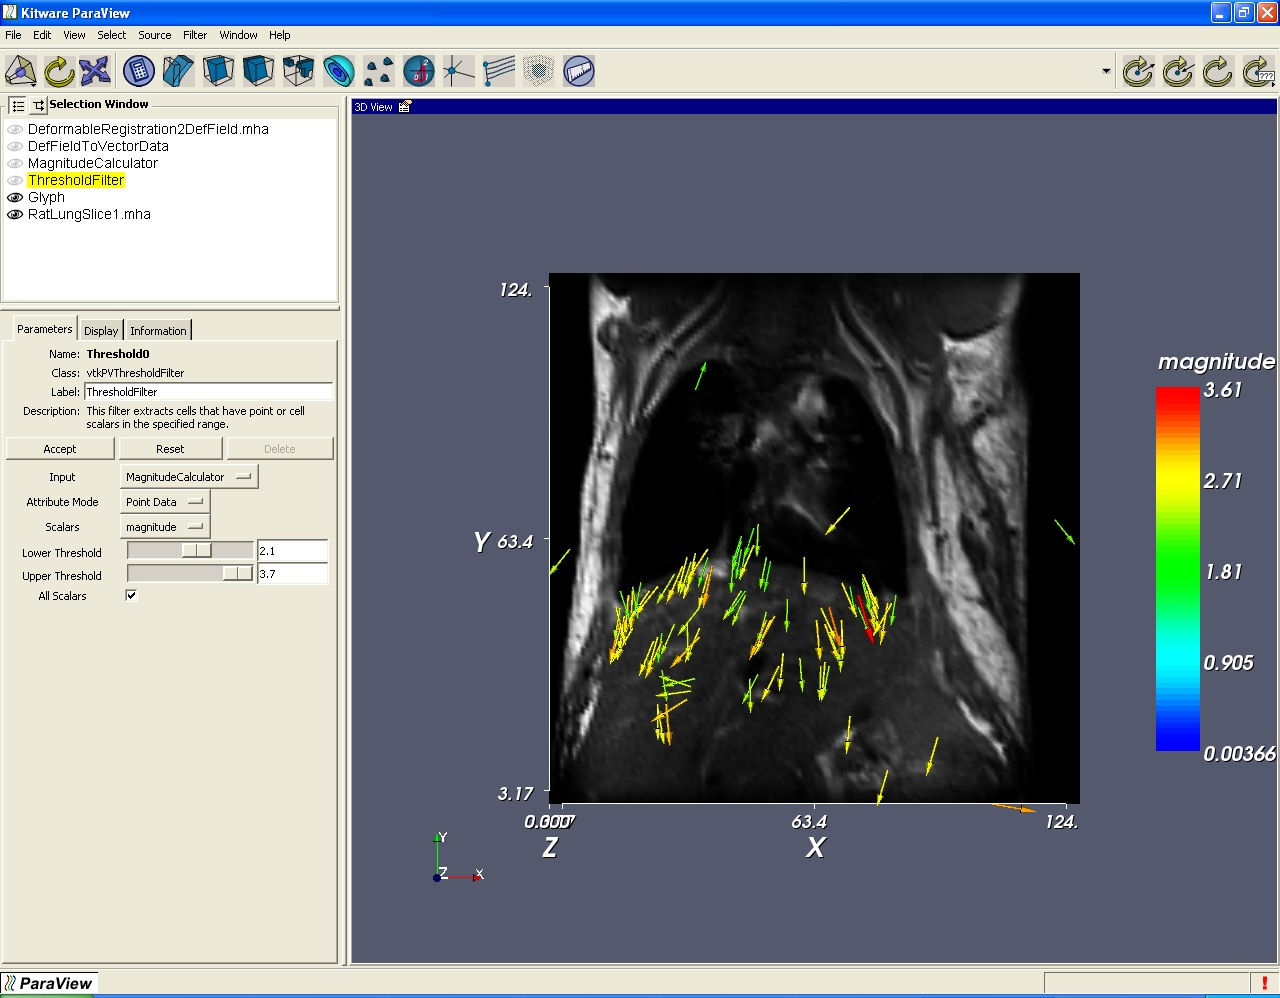
\includegraphics[width=\textwidth]{ParaviewScreenshot3.eps}
\itkcaption[Visualized Def field]{Deformation field visualized using Paraview after thresholding and subsampling.}
\label{fig:ParaviewScreenshot3}
\end{figure}



\subsection{Visualizing 3D deformation fields}
Let us create a 3D deformation field. We will use Thin Plate Splines to warp a 3D dataset and create a deformation field. We will pick a set of point landmarks and translate them to provide a specification of correspondences at point landmarks. Note that the landmarks have been picked randomly for purposes of illustration and are not intended to portray a true deformation. The landmarks may be used to produce a deformation field in several ways. Most techniques minimize some regularizing functional representing the irregularity of the deformation field, which is usually some function of the spatial derivatives of the field. Here will we use {\it thin plate splines}. Thin plate splines minimize the regularizing functional 

\begin{equation}
I[f(x,y)] = \iint (f^2_{xx} + 2 f^2_{xy} + f^2_{yy}) dx dy
\end{equation}
where the subscripts denote partial derivatives of f.

The code for this section can be found in Insight/Examples/Registration/ThinPlateSplineWarp.cxx

We may now proceed as before to visualize the deformation field using Paraview as shown in Figure \ref{fig:ParaviewScreenshot4}.

\begin{figure}
\center
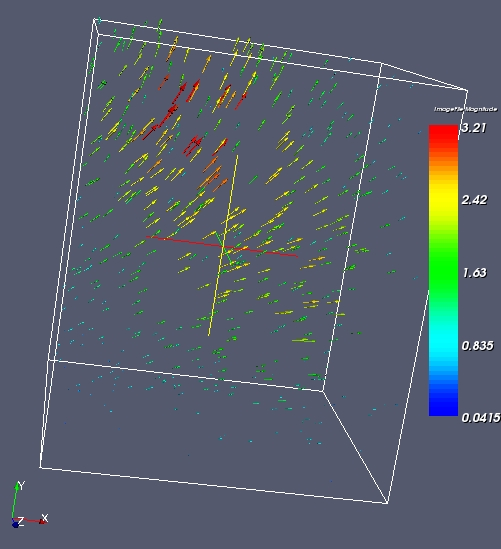
\includegraphics[width=0.7\textwidth]{ParaviewScreenshot4.eps}
\itkcaption[Visualized Def field4]{3D Deformation field visualized using Paraview.}
\label{fig:ParaviewScreenshot4}
\end{figure}




\fi

\ifitkFullVersion
%%%%%%%%%%%%%%%%%%%%%%%%%%%%%%%%%%%%%%%%%%%%%%%%%%%%%%%%%%%%%%%
%
%
%   This file is included in DeformableRegistration.tex
%
%   Labels and section entries are defined in that file.
%
%
%
%%%%%%%%%%%%%%%%%%%%%%%%%%%%%%%%%%%%%%%%%%%%%%%%%%%%%%%%%%%%%%
Let us register the deformed volumes generated by Thin plate warping in the
previous example using DeformableRegistration4.cxx. Since ITK is in general
N-dimensional, the only change in the example is to replace the
\code{ImageDimension} by 3.

The registration method uses B-splines and an LBFGS optimizer. The trace in
Table. \ref{tab:LBFGStrace} prints the trace of the optimizer through the
search space.

\begin{table}
\begin{center}
\begin{tabular}{\tableconfiguration}
\hline
\textbf{Iteration} &
\textbf{Function value} &
\textbf{$\|G\|$} &
\textbf{Step length} \\
\hline\hline
   1    &        156.981  &    14.911  & 0.202 \\
   2    &        68.956    &    11.774    &    1.500 \\
   3    &        38.146    &    4.802     &   1.500 \\
   4    &        26.690    &    2.515     &   1.500 \\
   5    &        23.295    &    1.106     &   1.500\\
   6    &        21.454    &    1.032     &   1.500\\
   7    &        20.322    &    1.557     &   1.500\\
   8    &        19.751    &    0.594     &   1.500\\
\hline
\end{tabular}
\end{center}
\itkcaption[LBFGS Optimizer trace]{LBFGS Optimizer trace.
\label{tab:LBFGStrace}}
\end{table}

Here $\|G\|$ is the norm of the gradient at the current estimate of the
minimum, $x$. ``Function Value" is the current value of the function, f(x).

The resulting deformation field that maps the moving to the fixed image is
shown in \ref{fig:DeformationFieldOutput}. A difference image of two slices
before and after registration is shown in
\ref{fig:DefRegistrationDiffScreenshot}. As can be seen from the figures, the
deformation field is in close agreement to the one generated from the Thin
plate spline warping.

\begin{figure}
\center
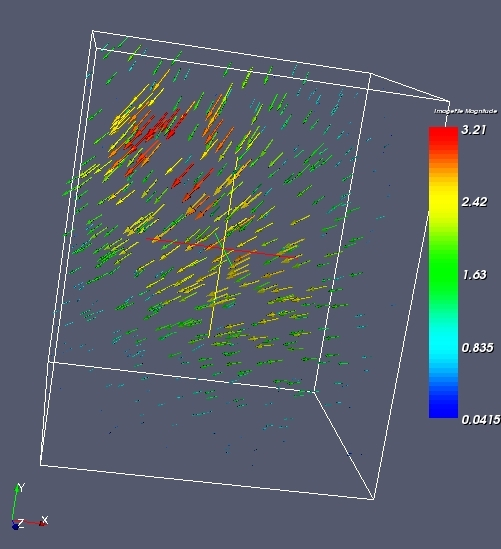
\includegraphics[width=0.6\textwidth]{ParaviewScreenshot5.eps}
\itkcaption[Deformation field output]{Resulting deformation field that maps the moving image to the fixed image.}
\label{fig:DeformationFieldOutput}
\end{figure}

\begin{figure}
\center

\includegraphics[width=0.44\textwidth]{DeformableRegistration4DiffBefore.eps}
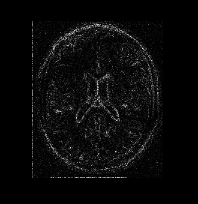
\includegraphics[width=0.44\textwidth]{DeformableRegistration4DiffAfter.eps}
\itkcaption[Difference image]{Difference image from a slice before and after registration.}
\label{fig:DefRegistrationDiffScreenshot}
\end{figure}



\fi


% the clearpage command helps to avoid orphans in the title of the next
% section.
\clearpage



\section{Model Based Registration}
\label{sec:ModelBasedRegistration}
\ifitkFullVersion
%%%%%%%%%%%%%%%%%%%%%%%%%%%%%%%%%%%%%%%%%%%%%%%%%%%%%%%%%%%%%%%
%
%
%   This file is included in Registration.tex
%
%   Lablels and section entries are defined in that file.
%
%
%
%%%%%%%%%%%%%%%%%%%%%%%%%%%%%%%%%%%%%%%%%%%%%%%%%%%%%%%%%%%%%%%

\itkpiccaption[Model to Image Registration Framework Components]{The basic components of model based registration are an image, a spatial object, a transform, a metric, an interpolator and an optimizer.\label{fig:ModelToImageRegistrationComponentsDiagram}}
\parpic(8cm,6cm)[r]{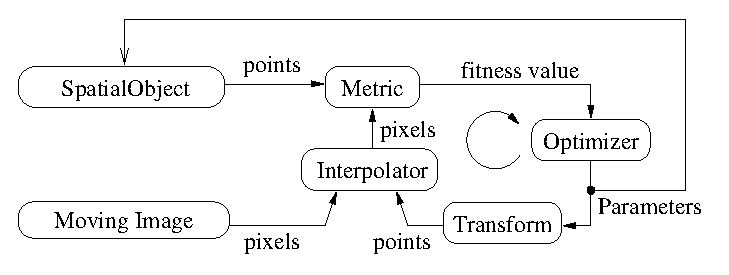
\includegraphics[width=7.5cm]{ModelToImageRegistrationComponentsDiagram.eps}}

This section introduces the concept of registering a geometrical model with an
image. We refer to this concept as \emph{Model Based Registration} but this may
not be the most widespread terminology. In this approach for registration, a
geometrical model is build first and a number of parameters are identified in
the model. Variations of these parameters make possible to adapt the model to
the particular morphology of a specific patient. The task of registration is
then to find the optimal combinations of the model parameters that will make
this model fit as a good representation of the anatomical structure contained
in an image. 


\begin{figure}
\center
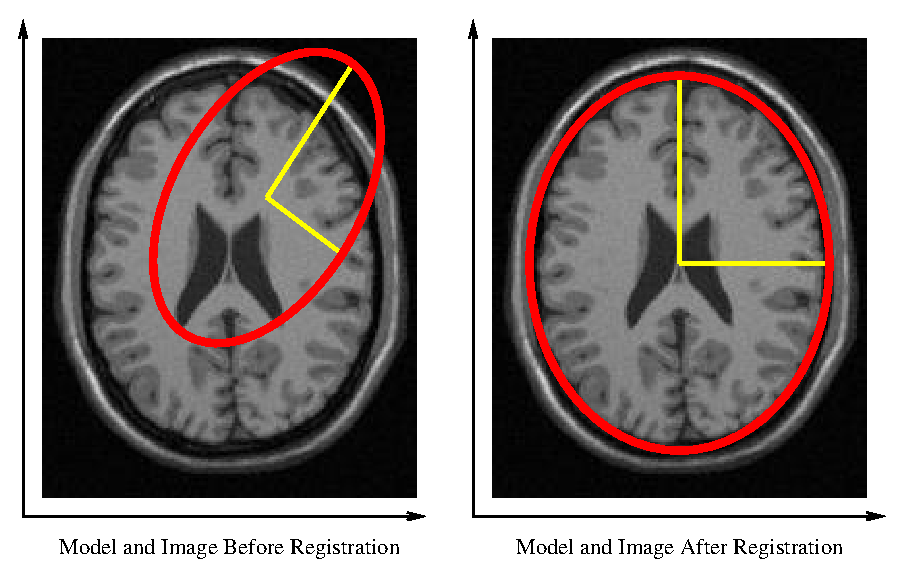
\includegraphics[width=\textwidth]{ModelToImageRegistrationConcept.eps}
\itkcaption[Model to Image Registration Framework Concept]{Basic concept of
  Model-to-Image registration.  A simplified geometrical model (ellipse) is
    registered against an anatomical structure (skull)  by applying a spatial
    transform and modifying the model internal parameters. This image is not
    the result of an actual registration, it is shown here only with the
    purpose of illustrating the concept of model to image registration.}
\label{fig:ModelToImageRegistrationConcept}
\end{figure}


For example, let's say that in the axial view of a brain image we can roughly
approximate the skull with an ellipse. The ellipse becomes our simplified
geometrical model, and registration is the task of finding the best center for
the ellipse, the measures of its axis lengths and its orientation on the plane.
This is illustrated in Figure~\ref{fig:ModelToImageRegistrationConcept}.  If we
compare this aproach with the Image-to-Image registration problem, we can see
that the main difference here is that in addition to mapping the spatial
position of the model, we can also customize internal parameters that change
its shape.

Figure~\ref{fig:ModelToImageRegistrationComponentsDiagram} illustrates the
major components of the registration framework in ITK when a model base
registration problem is configured. The basic input data for the registration
is provided by pixel data in an \doxygen{Image} and by geometrical data stored
in a \doxygen{SpatialObject}. A Metric has to be defined in order to evaluate
the fitness between the model and the image. This fitness value can be improved
by introducing variations in the spatial positioning of the
\doxygen{SpatialObject} and/or by changing its internal parameters. The search
space for the optimizer is now the composition of the transform parameter and
the shape internal parameters.

This same approach can be considered a segmentation technique, since once the
model has been optimally superimposed to the image we could label pixels
according to their associations with specific parts of the model. The
perpectives of model to image registration/segmentation are endless.  Probably
the main advantage of this approach is that, as opposed to image-to-image
registration, it actually provides \emph{Insight} into the anatomical structure
contained in the image. The adapted model becomes a condensed representation of
the essential elements of the anatomical structure.

ITK provides a hierarchy of classes intended to support the construction of
shape models. This hierarchy has the \doxygen{SpatialObject} as its base class.
A number of basic functionalities are defined at this level. For example, the
capacity to evaluate is a given point is \emph{inside} or \emph{outside} of the
model, the capability to form complex shapes by creating hierarchical
conglomerates of basic shapes and the support for basic spatial
parameterizations like scale, orientation and position.

The following sections present examples of the typical uses of these powerful
elements of the toolkit.

%\ifitkFullVersion
\input{ModelToImageRegistration1.tex} 
%\fi





\fi


\section{Point Set Registration}
\label{sec:PointSetRegistration}

PointSet-to-PointSet registration is a common problem in medical image
analysis. It usually arises in cases where landmarks are extracted from images
and are used for establishing the spatial correspondence between the images.
This type of registration can be considered to be the simplest case of
feature-based registration. In general terms, feature-based registration is
more efficient than the intensity based method that we have presented so far.
However, feature-base registration brings the new problem of identifying and
extracting the features from the images, which is not a minor challenge.

The two most common scenarios in PointSet to PointSet registration are

\begin{itemize}
\item Two PointSets with the same number of points, and where each point in one
set has a known correspondence to exactly one point in the second set.
\item Two PointSets without known correspondences between the points of one set
and the points of the other. In this case the PointSets may have different
numbers of points.
\end{itemize}

The first case can be solved with a closed form solution when we are dealing
with a Rigid or an Affine Transform~\cite{Horn1987}. This is done in ITK with
the class \doxygen{LandmarkBasedTransformInitializer}. If we are interested in
a deformable Transformation then the problem can be solved with the
\doxygen{KernelTransform} family of classes, which includes Thin Plate Splines
among others~\cite{Rohr2001}. In both circumstances, the availability o f
correspondences between the points make possible to apply a straight forward
solution to the problem.


The classical algorithm for performing PointSet to PointSet registration is the
Iterative Closest Point (ICP) algorithm.  The following examples illustrate how
this can be used in ITK.



\subsection{Point Set Registration in 2D}
\label{sec:PointSetRegistrationIn2D}

\ifitkFullVersion
\input{IterativeClosestPoint1.tex}
\fi




\subsection{Point Set Registration in 3D}
\label{sec:PointSetRegistrationIn3D}

\ifitkFullVersion
\input{IterativeClosestPoint2.tex}
\fi



\subsection{Point Set to Distance Map Metric}
\label{sec:PointSetToDistanceMapMetric}

\ifitkFullVersion
\input{IterativeClosestPoint3.tex}
\fi



\section{Registration Troubleshooting}
So you read the previous sections, you wrote the code, it compiles and links fine,
but when you run it the registration results are not what you were expecting.
In that case, this section is for you. This is a compilation of the most common
problems that users face when performing image registration. It provides explanations
on the potential sources of the problems, and advice on how to deal with those problems.

Most of the material in this section has been taken from frequently asked questions of
the ITK users list.


\subsection{Too many samples outside moving image buffer}


http://public.kitware.com/pipermail/insight-users/2007-March/021442.html

This is a common error message in image registration.

It means that at the current iteration of the optimization,
the two images as so off-registration that their spatial
overlap is not large enough for bringing them back into
registration.

The common causes of this problem are:

\begin{itemize}
\item Poor initialization:    You must initialize the transform properly.
Please read the ITK Software Guide http://www.itk.org/ItkSoftwareGuide.pdf  for
a description of the use of the CenteredTransformInitializer class.
\item Optimzer steps too large. If you optimizer takes steps that are too
large, it risks to become unstable and to send the images too far appart.  You
may want to start the optimizer with a maximum step lenght of 1.0, and only
increase it once you have managed to fine tune all other registration
parameters.

Increasing the step length makes your program faster, but it also makes it more
unstable.



\item Poor set up o the transform parameters scaling.  This is extremely
critical in registration. You must make sure that you balance the relative
difference of scale between the rotation parameters and the translation
parameters.

In typical medical datasets such as CT and MR, translations are measured in
millimeters, and therefore are in the range of -100:100, while rotations are
measured in radians, and therefore they tend to be in the range of   -1:1.


A rotation of 3 radians is catastrophic, while a translation of 3 millimeters
is rather inoffensive.  That difference in scale is the one that must be
accounted for.
\end{itemize}



\subsection{General heuristics for parameter fine-tunning}





http://public.kitware.com/pipermail/insight-users/2007-March/021435.html

Here is some advice on how to fine tune the parameters
of the registration process.


1) Set Maximum step length to 0.1 and do not change it
   until all other parameters are stable.

2) Set Minimum step length to 0.001 and do not change it.

   You could interpret these two parameters as if their
   units were radians. So, 0.1 radian = 5.7 degrees.


3) Number of histogram bins:

    First plot the histogram of your image using the
    example program in

    Insight/Examples/Statistics/ImageHistogram2.cxx

    In that program use first a large number  of bins
    (for example 2000) and identify the different
    populations of intensity level and to what anatomical
    structures they correspond.

    Once you identify the anatomical structures in the
    histogram, then rerun that same program with less
    and less number of bins, until you reach the minimun
    number of bins for which all the tissues that are important
    for your application, are still distinctly differentiated in the
    histogram.  At that point, take that number of bins and
    us it for your Mutual Information metric.


4)  Number of Samples:
    The trade-off with the number of samples is the following:

    a) computation time of registration is linearly proportional
       to the number of samples
                                                                                                                        b) the samples must be enough to significantly populate
                                                                                                                           the joint histogram.
                                                                                                                        c) Once the histogram is populated, there is not much
                                                                                                                           use in adding more samples.
Therefore do the following:

Plot the joint histogram of both images, using the number
of bins that you selected in item (3). You can do this by
modifying the code of the example:

Insight/Examples/Statistics/
ImageMutualInformation1.cxx
you have to change the code to print out the values
of the bins. Then use a plotting program such as gnuplot,
or Matlab, or even Excel and look at the distribution.
The number of samples to take must be enough
for producing the same "appearance" of the joint histogram.
As an arbitrary rule of thumb you may want to start using
a high number of samples (80% ~ 100%). And do not
change it until you have mastered the other parameters
of the registration.  Once you get your registration to converge
you can revisit the number of samples and reduce it in order
to make the registration run faster. You can simply reduce it
until you find that the registration becomes unstable. That's
your critical bound for the minimum number of samples.
Take that number and multiply it by the magic number 1.5,
to send it back to a stable region, or if your application is
really critical, then use an even higher magic number x2.0.

This is just engineering: you figure out what is the minimal
size of a piece of steel that will support a bridge, and then
you enlarge it to keep it away from the critical value.

5)  The MOST critical values of the registration process are the
scaling parameters that define the proportions between
the parameters of the transform. In your case, for an Affine
Transform in 2D, you have 6 parameters. The first four are
the ones of the Matrix, and the last two are the translation.
The rotation matrix value must be in the ranges of radians
which is typically [ -1 to 1 ], while the translation values are
in the ranges of millimeters (your image size units).
You want to start by setting the scaling of the matrix
parameters to 1.0, and the scaling of the Translation
parameters to the holy esoteric values:

1.0   /  (  10.0 * pixelspacing[0]  *  imagesize[0]  )
1.0   /  (  10.0 * pixelspacing[1]  *  imagesize[1]  )

This is telling the optimizer that you consider that rotating
the image by 57 degrees is as "significant" as translating
the image by half its physical extent.

Note that esoteric value has included the arbitrary number
10.0 in the denominator, for no other reason that we have
been lucky when using that factor. This of course is just a
supersticion, so you should feel free to experiment with
different values of this number.

Just keep in mind that what the optimizer will do is to
"jump" in a paramteric space of 6 dimension, and that the
component of the jump on every dimension will be proporitional
to 1/scaling factor * OptimizerStepLenght.     Since you put
the optimizer Step Length to 0.1, then the optimizer will start
by exploring the rotations at jumps of about 5degrees, which
is a conservative rotation for most medical applications.

If you have reasons to think that your rotations are larger or
smaller, then you should modify the scaling factor of the  matrix
parameters accordingly.

In the same way, if you thinkl that 1/10 of the image size is too
large as the first step for exploring the translations, then you
should modify the scaling of  translation parameters accordingly.



In order to drive all these you need to analyze the feedback that
the observer is providing you. For example, plot the metric values,
and plot the translation coordinates so that you can get a feeling
of how the registration is behaving.


Note also that image registration is not a science. it is a pure
engineerig practice, and therefore, there are no correct answers,
nor "truths" to be found. It is all about how much quality your want,
and how must computation time, and development time are you
willing to pay for that quality. The "satisfying" answer for your
specific application must be found by exploring the trade-offs
between the different parameters that regulate the image
registration process.

If you are proficient in VTK you may want to consider attaching
some visualization to the Event observer, so that you can have
a visual feedback on the progress of the registration. This is a
lot more productive than trying to interpret the values printed
out on the console by the observer.


\chapter{Segmentation}

Segmentation of medical images is a challenging task. A myriad of different
methods have been proposed and implemented in recent years. In spite of the
huge effort invested in this problem, there is no single approach that can
generally solve the problem of segmentation for the large variety of image
modalities existing today.

The most effective segmentation algorithms are obtained by carefully
customizing combinations of components. The parameters of these components are
tuned for the characteristics of the image modality used as input and the
features of the anatomical structure to be segmented.

The Insight Toolkit provides a basic set of algorithms that can be used to
develop and customize a full segmentation application. Some of the most
commonly used segmentation components are described in the following
sections.


\section{Region Growing}

Region growing algorithms have proven to be an effective approach for image
segmentation. The basic approach of a region growing algorithm is to start
from a seed region (typically one or more pixels) that are considered to be
inside the object to be segmented. The pixels neighboring this region are
evaluated to determine if they should also be considered part of the
object. If so, they are added to the region and the process continues as long
as new pixels are added to the region.  Region growing algorithms vary
depending on the criteria used to decide whether a pixel should be included
in the region or not, the type connectivity used to determine neighbors, and
the strategy used to visit neighboring pixels.

Several implementations of region growing are available in ITK.  This section
describes some of the most commonly used.

\subsection{Connected Threshold}

A simple criterion for including pixels in a growing region is to evaluate
intensity value inside a specific interval.

\label{sec:ConnectedThreshold}
\ifitkFullVersion
\input{ConnectedThresholdImageFilter.tex}
\fi

\subsection{Otsu Segmentation}
Another criterion for classifying pixels is to minimize the error of misclassification.
The goal is to find a threshold that classifies the image into two clusters such that
we minimize the area under the histogram for one cluster that lies on the other cluster's
side of the threshold. This is equivalent to minimizing the within class variance
or equivalently maximizing the between class variance.

\label{sec:OtsuThreshold}
\ifitkFullVersion
\input{OtsuThresholdImageFilter.tex}
\fi

\label{sec:OtsuMultipleThreshold}
\ifitkFullVersion
\input{OtsuMultipleThresholdImageFilter.tex}
\fi

\subsection{Neighborhood Connected}
\label{sec:NeighborhoodConnectedImageFilter}
\ifitkFullVersion
\input{NeighborhoodConnectedImageFilter.tex}
\fi


\subsection{Confidence Connected}
\label{sec:ConfidenceConnected}
\ifitkFullVersion
\input{ConfidenceConnected.tex}
\subsubsection{Application of the Confidence Connected filter on the Brain Web Data}
This section shows some results obtained by applying the Confidence Connected filter on the BrainWeb database. The filter was applied on a 181 $\times$ 217 $\times$ 181 crosssection of the {\it brainweb165a10f17} dataset. The data is a MR T1 acquisition, with an intensity non-uniformity of 20\% and a slice thickness 1mm. The dataset may be obtained from
\code{http://www.bic.mni.mcgill.ca/brainweb/} or
\code{https://data.kitware.com/\#folder/5882712d8d777f4f3f3072df}

The previous code was used in this example replacing the image dimension by 3.
Gradient Anistropic diffusion was applied to smooth the image. The filter used 2 iterations, a time step of 0.05 and a conductance value of 3. The smoothed volume was then segmented using the Confidence Connected approach. Five seed points were used at coordinate locations (118,85,92), (63,87,94), (63,157,90), (111,188,90), (111,50,88). The ConfidenceConnnected filter used the parameters, a neighborhood radius of 2, 5 iterations and an $f$ of 2.5 (the same as in the previous example). The results were then rendered using VolView.

Figure \ref{fig:3DregionGrowingScreenshot1} shows the rendered volume. Figure \ref{fig:SlicesBrainWeb} shows an axial, saggital and a coronal slice of the volume.

\begin{figure}
\centering
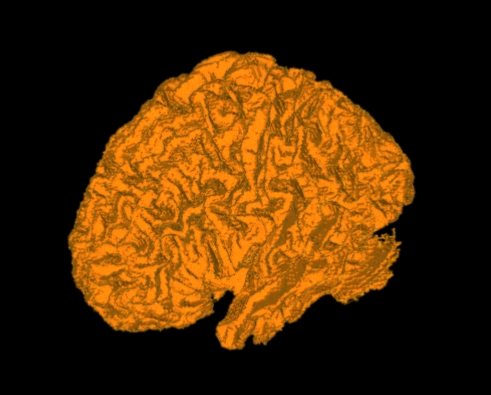
\includegraphics[width=0.6\textwidth]{3DregionGrowingScreenshot1.eps}
\itkcaption[Whitematter Confidence Connected segmentation.]{White matter segmented using Confidence Connected region growing.}
\label{fig:3DregionGrowingScreenshot1}
\end{figure}

\begin{figure}
\centering

\includegraphics[width=\textwidth]{SlicesBrainWebConfidenceConnected.eps}
\itkcaption[Axial, sagittal, and coronal slice of Confidence Connected segmentation.]{Axial, sagittal and coronal slice segmented using Confidence Connected region growing.}
\label{fig:SlicesBrainWeb}
\end{figure}

\fi




\subsection{Isolated Connected}
\label{sec:IsolatedConnected}
\ifitkFullVersion
\input{IsolatedConnectedImageFilter.tex}
\fi


\subsection{Confidence Connected in Vector Images}
\label{sec:VectorConfidenceConnected}
\ifitkFullVersion
\input{VectorConfidenceConnected.tex}
\fi


\section{Segmentation Based on Watersheds}
\label{sec:WatershedSegmentation}
\ifitkFullVersion
\input WatershedSegmentation.tex
\fi


% the clearpage command helps to avoid orphans in the title of the next
% section.
\clearpage

\section{Level Set Segmentation}
\label{sec:LevelSetsSegmentation}
\ifitkFullVersion
%%%%%%%%%%%%%%%%%%%%%%%%%%%%%%%%%%%%%%%%%%%%%%%%%%%%%%%%%%%%%%%%%%%%%%%%
%
%
%     This file is included from the file   Segmentation.tex
% 
%     Section tag and label are placed in this top file.
%
%
%
%%%%%%%%%%%%%%%%%%%%%%%%%%%%%%%%%%%%%%%%%%%%%%%%%%%%%%%%%%%%%%%%%%%%%%%%



\itkpiccaption[Zero Set Concept]{Concept of Zero Set in a Level Set.\label{fig:LevelSetZeroSet}}
\parpic(9cm,6cm)[r]{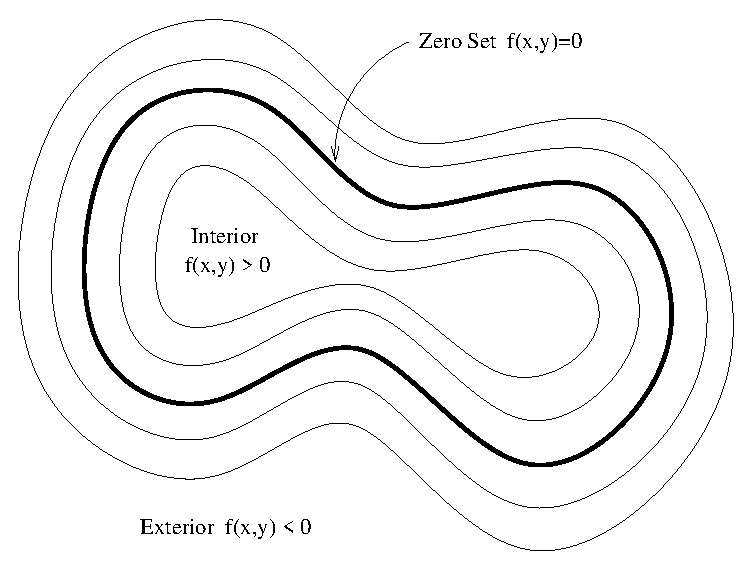
\includegraphics[width=8cm]{LevelSetZeroSet.eps}}

The paradigm of Level Set is a numerical method for tracking the evolution of
contours and surfaces. Instead of manipulating the contour directly, the
contour is embedded as the zero level set of a higher dimensional function
called the level-set function, $\psi(\bf{X},t)$. The level-set function is then
evolved under the control of a differential equation.  At any time, the evolving
contour can be obtained by extracting the zero level-set $\Gamma(\bf(X),t) =
\{\psi(\bf{X},t) = 0\}$ from the output.  The main advantages of using level
sets is that arbitrarily complex shapes can be modeled and topological
changes such as merging and splitting are handled implicitly. 

Level sets can be used for image segmentation by using image-based features such
as mean intensity, gradient and edges in the governering differential equation. 
In a typical approach, a contour is initialized by a user and is then evolved 
until it fits the form of an anatomical structure in the image. 
Many different implementations and variants of this basic concept have been
published in the literature. An overview of the field has been made by Sethian
\cite{Sethian1996}. 

The following sections introduce practical examples of some
of the Level Set segmentation methods available in ITK.  The remainder of this
section describes features common to all of these filters except the
\code{FastMarchingImageFilter}, which is derived from a different code
framework.  Understanding these features will aid in using the filters
more effectively.

Each filter makes use of a generic level-set equation to compute the update to
the solution $\psi$ of the partial differential equation.

\begin{equation}
\label{eqn:LevelSetEquation}
\frac{d}{dt}\psi = -\alpha \mathbf{A}(\mathbf{x})\cdot\nabla\psi - \beta
  P(\mathbf{x})\mid\nabla\psi\mid + \gamma Z(\mathbf{x})\kappa
\end{equation}
 
where $\mathbf{A}$ is an advection term, $P$ is a propagation (expansion) term,
and $Z$ is a spatial modifier term for the mean curvature $\kappa$.  The scalar
constants $\alpha$, $\beta$, and $\gamma$ weight the relative influence of
each of the terms on the movement of the interface.  A segmentation filter may
use all of these terms in its calculations, or it may omit one or more terms.
If a term is left out of the equation, then setting the corresponding scalar
constant weighting will have no effect.

All of the level-set based segmentation filters \emph{must} operate with
floating point precision to produce valid results.  The third, optional
template parameter is the \emph{numerical type} used for calculations and as
the output image pixel type.  The numerical type is \code{float} by default,
but can be changed to \code{double} for extra precision.  A user-defined,
signed floating point type that defines all of the necessary arithmetic
operators and has sufficient precision is also a valid choice.  You should not
use types such as \code{int} or \code{unsigned char} for the numerical
parameter.  If the input image pixel types do not match the numerical type,
those inputs will be cast to an image of appropriate type when the filter is
executed.

Most filters require two images as input, an initial model $\psi(\bf{X}, t=0)$,
and a \emph{feature image}, which is either the image you wish to segment or
some preprocessed version therof.  You must specify the isovalue that
represents the surface $\Gamma$ in your initial model. The single image output of
each filter is the function $\psi$ at the final time step.  It is important to
note that the contour representing the surface $\Gamma$ is the zero level-set
of the output image, and not the isovalue you specified for the initial model.
To represent $\Gamma$ using the original isovalue, simply add that value back
to the output.

The solution $\Gamma$ is calculated to subpixel precision.  The best discrete
approximation of the surface is therefore the set of grid positions closest to
the zero-crossings in the image, as shown in
figure~\ref{fig:LevelSetSegmentationFigure1}.  The
\code{itk::ZeroCrossingImageFilter} operates by finding exactly those grid 
positions and can be used to extract the surface. 

\begin{figure}
\centering
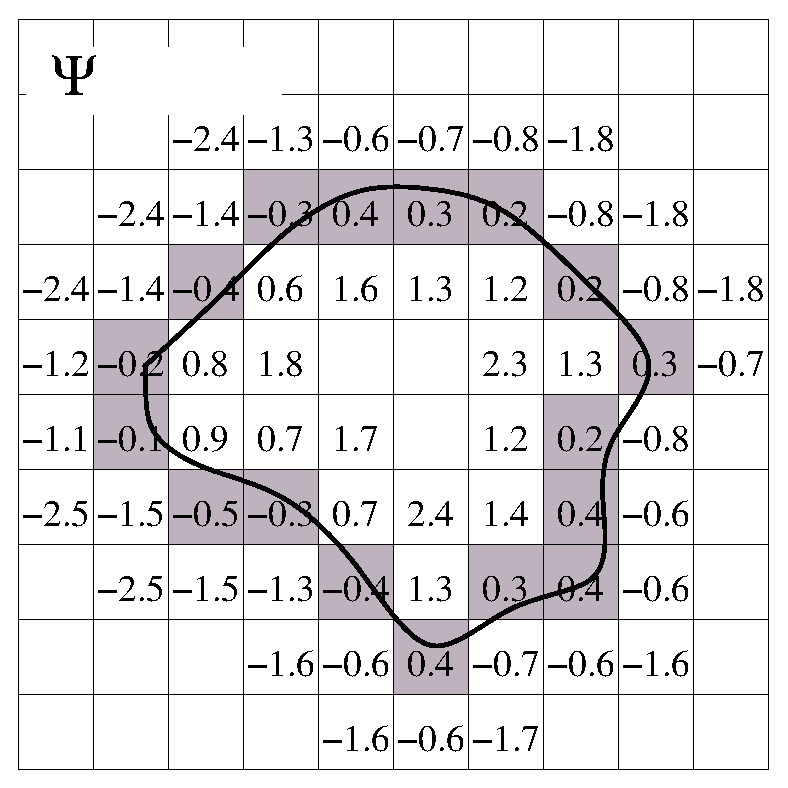
\includegraphics[width=0.4\textwidth]{LevelSetSegmentationFigure1.eps}
\itkcaption[Grid position of the embedded level-set surface.]{The implicit level
set surface $\Gamma$ is the black line superimposed over the image grid.  The location
of the surface is interpolated by the image pixel values.  The grid pixels
closest to the implicit surface are shown in gray. }
\protect\label{fig:LevelSetSegmentationFigure1}
\end{figure}

There are two important considerations when analyzing the processing time for
any particular level-set segmentation task: the surface area of the evolving
interface and the total distance that the surface must travel.  Because the
level-set equations are usually solved only at pixels near the surface (fast
marching methods are an exception), the time taken at each iteration depends on
the number of points on the surface.  This means that as the surface grows, the
solver will slow down proportionally.  Because the surface must evolve slowly
to prevent numerical instabilities in the solution, the distance the surface
must travel in the image dictates the total number of iterations required.

Some level-set techniques are relatively insensitive to initial conditions and are
therefore suitable for region-growing segmentation. Other techniques, like
\code{itk::LaplacianSegmentationLevelSetImageFilter}, can easily become
``stuck'' on image features close to their initialization and should be used
only when a reasonable prior segmentation is available as the initialization.
For best efficiency, your initial model of the surface should be the
best guess possible for the solution.  When extending the example applications
given here to higher dimensional images, for example, you can improve results
and dramatically decrease processing time by using a multi-scale
approach. Start with a downsampled volume and work back to the full resolution
using the results at each intermediate scale as the initialization for the next
scale.


\subsection{Fast Marching Segmentation}
\label{sec:FastMarchingImageFilter}

\ifitkFullVersion
\input{FastMarchingImageFilter.tex}
\fi



\subsection{Shape Detection Segmentation}
\label{sec:ShapeDetectionLevelSetFilter}

\ifitkFullVersion
\input{ShapeDetectionLevelSetFilter.tex}
\fi


\subsection{Geodesic Active Contours Segmentation}
\label{sec:GeodesicActiveContourImageFilter}

\ifitkFullVersion
\input{GeodesicActiveContourImageFilter.tex}
\fi


\subsection{Threshold Level Set Segmentation}
\label{sec:ThresholdSegmentationLevelSetImageFilter}
\ifitkFullVersion
\input{ThresholdSegmentationLevelSetImageFilter.tex}
\fi

\subsection{Canny-edge Level Set Segmentation}
\label{sec:CannySegmentationLevelSetImageFilter}
\ifitkFullVersion
\input{CannySegmentationLevelSetImageFilter.tex}
\fi

\subsection{Laplacian Level Set Segmentation}
\label{sec:LaplacianSegmentationLevelSetImageFilter}
\ifitkFullVersion
\input{LaplacianSegmentationLevelSetImageFilter.tex}
\fi



\fi


%HACK: TODO Review what happended to these.
%REMOVED PATENTED: \section{Hybrid Methods}
%REMOVED PATENTED: \label{sec:HybridSegmentationMethods}
%REMOVED PATENTED:
%REMOVED PATENTED: \ifitkFullVersion
%REMOVED PATENTED: %%%%%%%%%%%%%%%%%%%%%%%%%%%%%%%%%%%%%%%%%%%%%%%%%%%%%%%%%%%%%%%%%%%%%%%%
%
%
%     This file is included from the file   Segmentation.tex
% 
%     Section tag and label are placed in this top file.
%
%
%
%%%%%%%%%%%%%%%%%%%%%%%%%%%%%%%%%%%%%%%%%%%%%%%%%%%%%%%%%%%%%%%%%%%%%%%%

\subsection{Introduction}
\label{sec:HybridSegmentationIntroduction}


Hybrid methods for automated segmentation of radiological patient data and the 
Visible Human data integrate boundary-based and region-based segmentation methods 
that amplify the strength but reduces the weakness of both approaches.The novelty 
comes from combining a region-based segmentation methods, the fuzzy connectedness 
and Voronoi Diagram classification with a boundary-based deformable model 
segmentation, to develop hybrid methods that yield high precision, accuracy and 
efficiency.The synergy between fundamentally different methodologies tends to 
result in robustness and higher segmentation quality. We built Hybrid Segmentation 
Engine,  Figure \ref{fig:ComponentsofaHybridSegmentationApproach}, that consists of modules 
representating component segmentation methods (itk filters). We can derive a variety 
of hybrid segmentation methods from the modules. It should be noted that under Fuzzy 
Connectedness module and Deformable Models module, we checked in into the itk a number 
of filters in each of the categories, respectively. Below, we decribe two examples of
hybrid segmentation methods, derived from the Hybrid segmentation Engine: Hybrid 
Method 1: Integration of Fuzzy Connectedness and Voronoi Diagram Classification;
Hybrid Method 2: Integration of Gibbs prior and Deformable Models.
Details on the concepts behind those methods have been discussed in the
literature
\cite{Angelini2002,Udupa2002,Jin2002,Imielinska2001,Imielinska2000a,Imielinska2000b}



\subsection{FuzzyConectedness and VoronoiDiagramClassification}
\label{sec:HybridMethod1}

In this section, we present a hybrid segmentation method that requires minimal
manual initialization, where we integrate the fuzzy connectedness segmentation
and Voronoi Diagram Classification. We start with fuzzy connectedness filter
to generate a sample of tissue from a region to be segmented. From the sample,
we derive automatically, homogeneity statistics that constitute homogeneity
operator to be used in the next stage of the method. The output of the fuzzy 
connectedness filter is used as a prior for the Voronoi Diagram Classification 
filter that performs iterative subdivision and classification of the segmented
image that results in an estimation of the boundary. The output of this filter
is a 3D binary image that can be used to display the 3D result of the
segmentation, or passed to another filter (e.g. Deformable Model) for further
improvement of the final segmentation. Details describing the concepts behind those methods 
have been published in
\cite{Angelini2002,Udupa2002,Jin2002,Imielinska2001,Imielinska2000a,Imielinska2000b}

In Figure \ref{fig:UMLClassDiagramoftherFuzzyConnectednessFilter}, we describe 
base class for simple fuzzy connectedness segmentation. This method is non-scale 
based, non-iterative and requires only one seed to initialize it. We define affinity 
between two nearby elements in a image (e.g. pixels, voxels) via a degree of adjacency, 
similarity of their intensity values, and their similarity with the estimated object. 
The closer the elements are and more similar their intensities are, the greater is 
the affinity between them. We compute the strength of a path and fuzzy connectedness 
between each two pixels (voxels) in the segmented image from the fuzzy affinity. 
Computation of fuzzy connectedness value of each pixel (voxel) is implemented
by selecteing a seed point and using dynamic programming. The result constitutes the fuzzy
map. Thresholding of the fuzzy map gives a segmented object that is strongly connected
to the seed point (for more details, see \cite{Udupa1996}). We checked in two fuzzy 
connectedness filters: the itkSimpleFuzzyConnectednessScalarImageFilter that is an
implementation of the fuzzy connectedness segmentation of single channel (gray scale) 
image;itkSimpleFuzzyConnectednessRGBImageFilter that is an implementation of fuzzy
connectedness implementation of three-channel (RGB) image. Other classes can be derived 
from the base class by defining other affinity function, and targeting multi-channel
images with and arbitrary number of channels. It has to be noted, that the simple fuzzy 
connectedness filter can be used as a stand-alone segmentation method,
as it is described in the diagram in Figure 
\ref{fig:UMLCollaborationDiagramoftheFuzzyConnectednessFilter}.

In Figure \ref{fig:UMLVoronoiSegmentationClassFilter} we present base class for
Voronoi Diagram Clasification. We initialize the method with a number of random
seed points and compute Voronoi Diagram over the segmented 2D image. Each
Voronoi region, in teh subdivision, is classified as internal or external,
based on the homogeneity operator derived from the fuzzy connectedness
algorithm.  We define boundary regions as the external regions that are
adjacent to the internal regions.  We subdivide further the boundary regions
by adding seed points to the regions. We converge to the final segmentation
using simple stopping criterium (for details, see \cite{Imielinska2001}). We
implemneted two Voronoi Diagram filters: the
itkVoronoiSegmentationImageFilter that is dedicated to process single channel
(gray scale) images; the itkVoronoiSegmentationRGBImageFilter that segments
three-channel (RGB) images. Other classes can be derivedfrom the base class
by defining other homogeneity measurements, and targeting multichannel images
with and arbitrary number of channels.  The other classes that are used for
computing 2D Voronoi Diagram, are shown in Figure
\ref{fig:UMLClassesforImplementationofVoronoiDiagramFilter}. We note that the
Voronoi Diagram Filter can be used as a stand-alone segmentation method, as
it is depicted in Figure
\ref{fig:UMLCollaborationDiagramoftheVoronoiSegmentationFilter}.

 We present in Figure \ref{fig:UMLHybridMethodDiagram1} and Figure
 \ref{fig:UMLHybridMethodDiagram2} diagrams for hybrid segmentation methods
 that integrate: fuzzy connectedness with Voronoi Diagram; and fuzzy
 connectedness, Voronoi Diagram with Deformable Models, respectively.


%%%%%%%%%%%%%%%%%%%%%%%%%%%%%%%%%%%%%%%%%%%%%%%%%%%%%%%%%%%%%%%%%
%
%  Here is an example of how to include diagram in a figure
%
%  The file HybridSegmentationDiagram1.fig should be in the "Art"
%  directory. CMake will convert it to EPS before running latex. 
%
%%%%%%%%%%%%%%%%%%%%%%%%%%%%%%%%%%%%%%%%%%%%%%%%%%%%%%%%%%%%%%%%%

\begin{figure}
\center
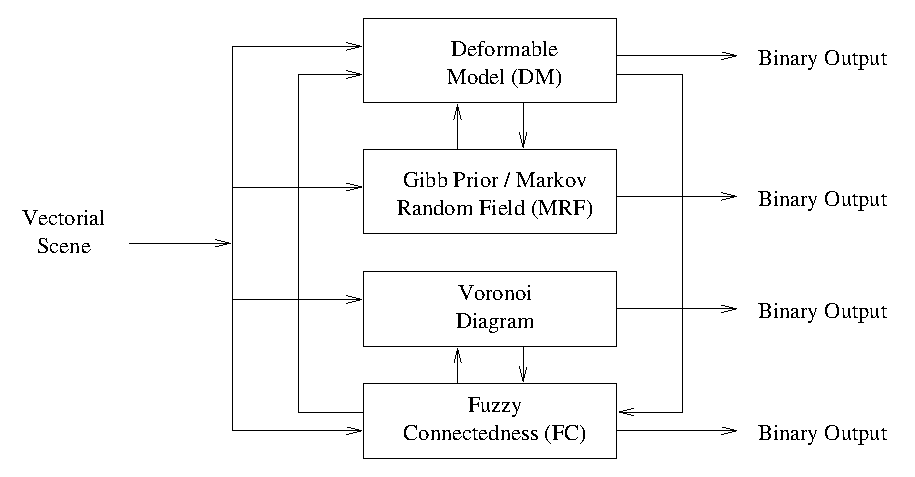
\includegraphics[width=14cm]{HybridSegmentationEngine1.eps}
\caption{Hybrid Segmentation Engine}
\label{fig:ComponentsofaHybridSegmentationApproach}
\end{figure}


\begin{figure}
\center
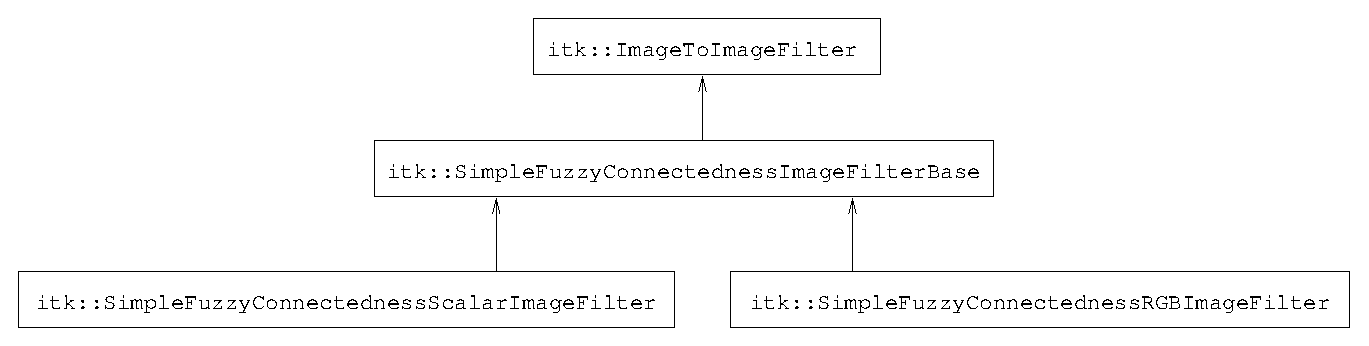
\includegraphics[width=14cm]{FuzzyConnectednessClassDiagram1.eps}
\caption{Diagram of the FuzzyConnectedness filter}
\label{fig:UMLClassDiagramoftherFuzzyConnectednessFilter}
\end{figure}


\begin{figure}
\center
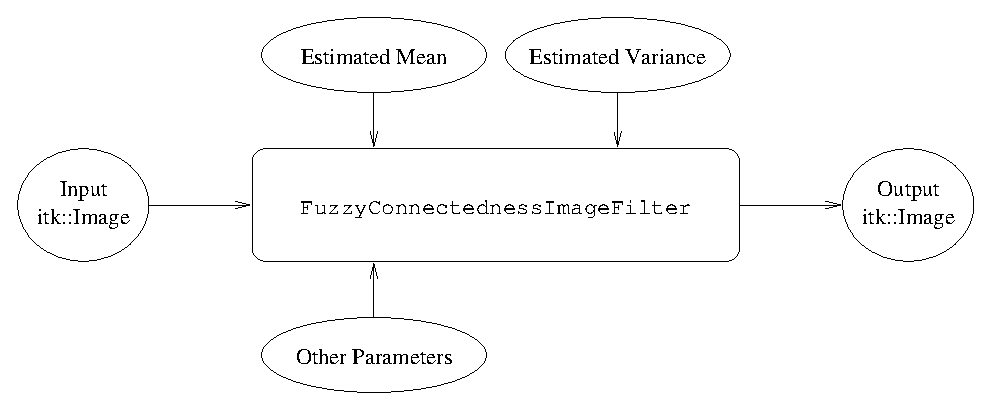
\includegraphics[width=14cm]{FuzzyConnectednessCollaborationDiagram1.eps}
\caption{Diagram Of Stand-Alone Fuzzy Connectedness Segmentation}
\label{fig:UMLCollaborationDiagramoftheFuzzyConnectednessFilter}
\end{figure}

\begin{figure}
\center
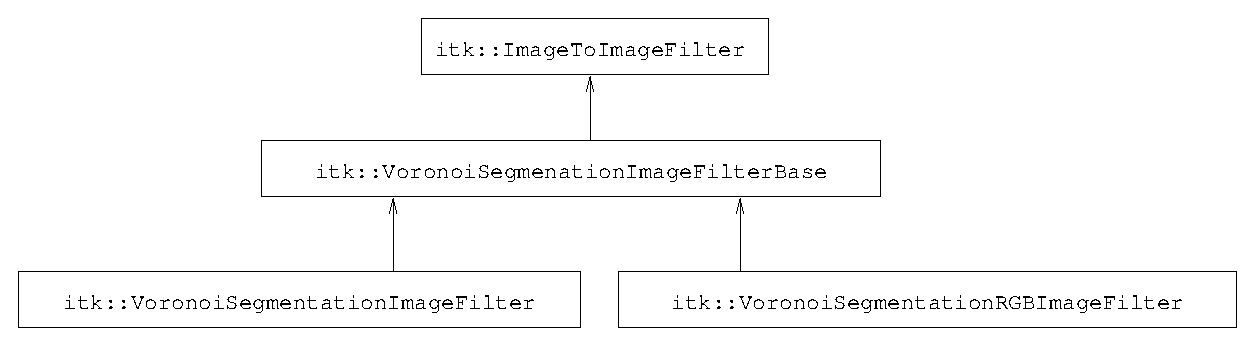
\includegraphics[width=14cm]{VoronoiSegmentationClassDiagram1.eps}
\caption{Diagram of the Voronoi Diagram Classification filter}
\label{fig:UMLVoronoiSegmentationClassFilter}
\end{figure}

\begin{figure}
\center
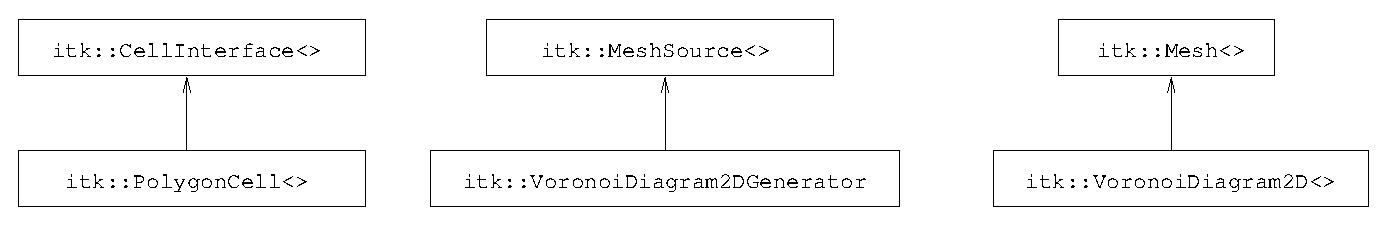
\includegraphics[width=14cm]{VoronoiSegmentationCollaborationDiagram1.eps}
\caption{Classes for Implementation of Voronoi Diagram Filter}
\label{fig:UMLClassesforImplementationofVoronoiDiagramFilter}
\end{figure}


\begin{figure}
\center
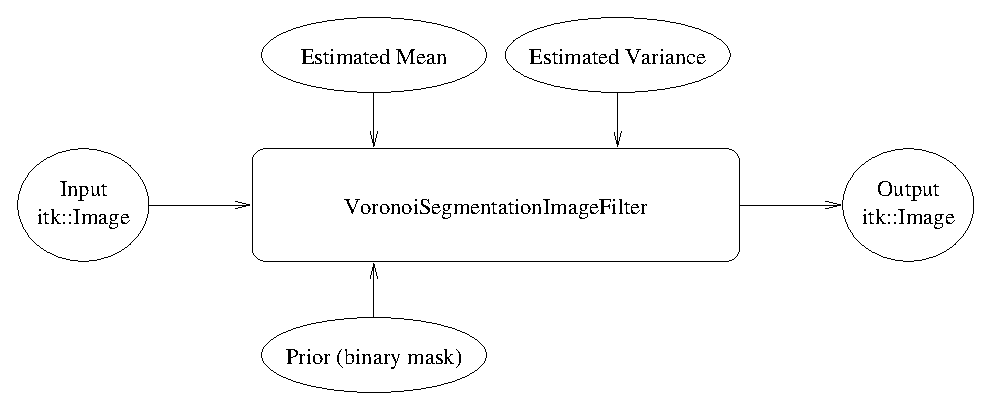
\includegraphics[width=14cm]{VoronoiSegmentationCollaborationDiagram2.eps}
\caption{Diagram Of Stand-Alone Voronoi Diagram Segmentation}
\label{fig:UMLCollaborationDiagramoftheVoronoiSegmentationFilter}
\end{figure}


\begin{figure}
\center
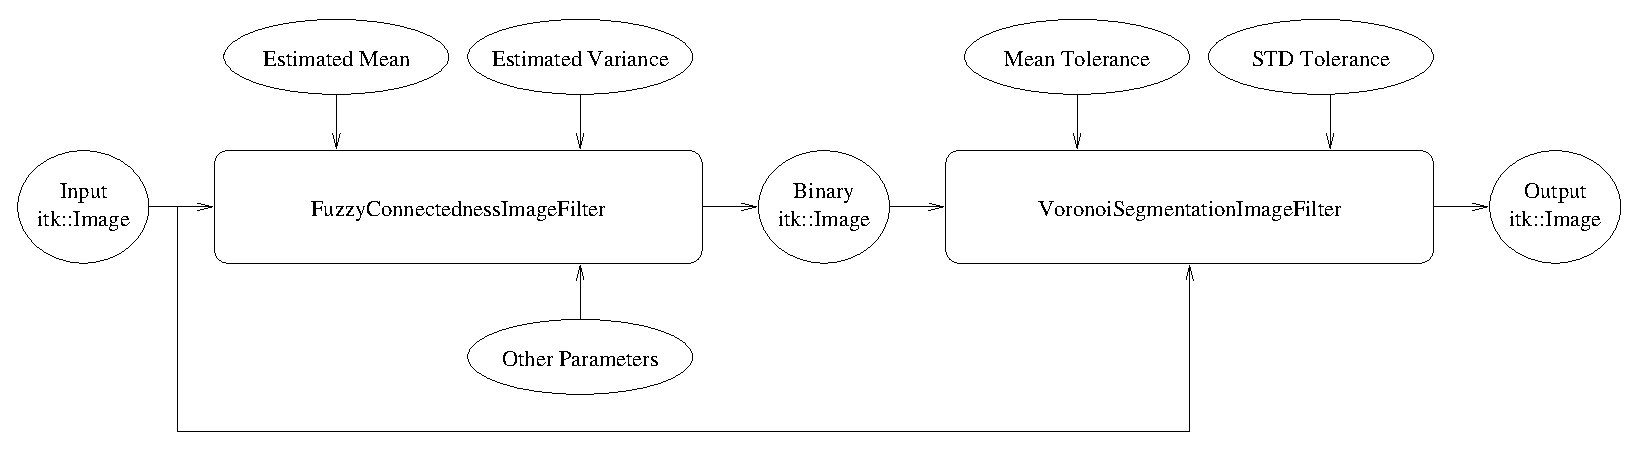
\includegraphics[width=14cm]{FuzzyVoronoiCollaborationDiagram1.eps}
\caption{Integration of Fuzzy Connectedness with Voronoi Diagram Classification}
\label{fig:UMLHybridMethodDiagram1}
\end{figure}

\begin{figure}
\center
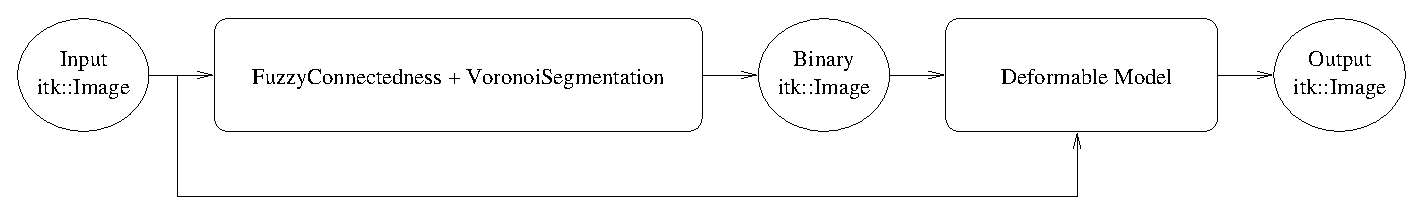
\includegraphics[width=14cm]{FuzzyVoronoiDeformableCollaborationDiagram1.eps}
\caption{Integration of Fuzzy Connectedness, Voronoi Diagram, and Deformable Models}
\label{fig:UMLHybridMethodDiagram2}
\end{figure}



\subsubsection{Example of an Hybrid segmentation Method}
\label{sec:HybridMethod1:Example}

%\ifitkFullVersion
\input{HybridSegmentationFuzzyVoronoi.tex}
%\fi



\subsection{Deformable models and Gibbs Prior}

Another combination that can be used in an hybrid segmentation method it the
set of Gibbs prior filters with Deformable models.

\subsubsection{Deformable Model}
%\ifitkFullVersion
\input{DeformableModel1.tex}
%\fi


\subsubsection{Gibbs Prior Image Filter}
%\ifitkFullVersion
\input{GibbsPriorImageFilter1.tex}
%\fi


%REMOVED PATENTED: \fi


\section{Feature Extraction}
\label{sec:FeatureExtractionMethods}

\ifitkFullVersion
%%%%%%%%%%%%%%%%%%%%%%%%%%%%%%%%%%%%%%%%%%%%%%%%%%%%%%%%%%%%%%%%%%%%%%%%
%
%
%     This file is included from the file   Segmentation.tex
% 
%     Section tag and label are placed in this top file.
%
%
%
%%%%%%%%%%%%%%%%%%%%%%%%%%%%%%%%%%%%%%%%%%%%%%%%%%%%%%%%%%%%%%%%%%%%%%%%


Extracting salient features from images is an important task on image
processing.  It is typicaly used for guiding segmentation methods, perparing
data for registration methods, or as a mechanism for recognimizing anatomical
structures in images.

The following section introduce some of the feature extraction methods 
available in the toolkit.


\subsection{Hough Transform}
\label{sec:HoughtLineExtraction}

The Hough transfomr is a widely used technique for detection of geometrical
features in images. It is based on mapping the image into a parameteric space
in which it may be easier to identify if particular geometrical features are
present in the image. The transformation is specific for each desired
geometrical shape. 

\subsubsection{Line Extraction}
\label{sec:HoughtLineExtraction}

\ifitkFullVersion
\input{HoughTransform2DLinesImageFilter.tex}
\fi



\subsubsection{Circle Extraction}
\label{sec:HoughtCircleExtraction}

\ifitkFullVersion
%\input{HoughTransform2DLinesImageFilter.tex}
\fi




\fi

\chapter{Statistics}
\label{sec:StaisticsFramework}

This chapter introduces the statistics functionalities in Insight. The
statistics subsystem's primary purpose is to provide general capabilities
for statistical pattern classification. However, its use is not limited
for classification. Users might want to use data containers and
algorithms in the statistics subsystem to perform other statistical
analysis or to preprocessor image data for other tasks.

The statistics subsystem mainly consists of three parts: data container
classes, statistical algorithms, and the classification framework. In this
chapter, we will discuss each major part in that order.

\section{Data Containers}
\label{sec:StatisticsDataContainer}

An \subdoxygen{Statistics}{Sample} object is a data container of elements
that we call \emph{measurement vectors}. A measurement vector is an array of
values (of the same type) measured on an object (In images, it can be a
vector of the gray intensity value and/or the gradient value of a
pixel). Strictly speaking from the design of the Sample class, a measurement
vector can be any class derived from \doxygen{FixedArray}, including
FixedArray itself.

\begin{figure}
  \centering
  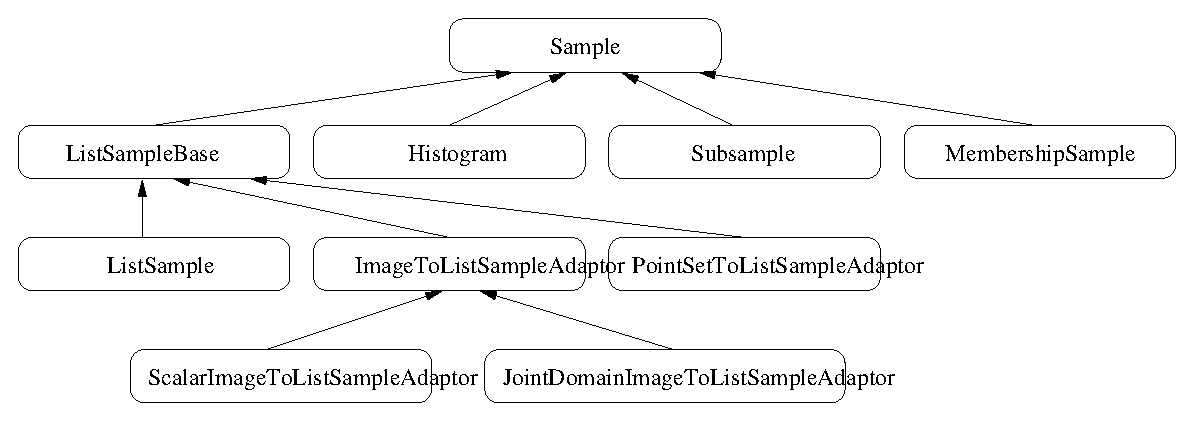
\includegraphics[width=0.9\textwidth]{SampleInheritanceTree.eps}
  \itkcaption[Sample class inheritance tree]{Sample class inheritance diagram.}
  \protect\label{fig:SampleInheritanceTree}
\end{figure}

\subsection{Sample Interface}
\label{sec:SampleInterface}

\ifitkFullVersion
\input{ListSample.tex}
\fi

\subsection{Sample Adaptors}
\label{sec:SampleAdaptors}

There are two adaptor classes that provide the common
\subdoxygen{Statistics}{Sample} interfaces for \doxygen{Image} and
\doxygen{PointSet}, two fundamental data container classes found in ITK. The
adaptor classes do not store any real data elements themselves. These data
comes from the source data container plugged into them. First, we will
describe how to create an
\subdoxygen{Statistics}{ImageToListSampleAdaptor} and then an
\subdoxygen{Statistics}{PointSetToListSampleAdaptor} object.

\subsubsection{ImageToListSampleAdaptor}
\label{sec:ImageToListSampleAdaptor}

\ifitkFullVersion
\input{ImageToListSampleAdaptor.tex}
\fi

\subsubsection{PointSetToListSampleAdaptor}
\label{sec:PointSetToListSampleAdaptor}

\ifitkFullVersion
\input{PointSetToListSampleAdaptor.tex}
\fi

\ifitkFullVersion
\input{PointSetToAdaptor.tex}
\fi


\subsection{Histogram}
\label{sec:Histogram}

\ifitkFullVersion
\input{Histogram.tex}
\fi

\subsection{Subsample}
\label{sec:Subsample}

\ifitkFullVersion
\input{Subsample.tex}
\fi

\subsection{MembershipSample}
\label{sec:MembershipSample}

\ifitkFullVersion
\input{MembershipSample.tex}
\fi

\subsection{MembershipSampleGenerator}
\label{sec:MembershipSampleGenerator}

\ifitkFullVersion
\input{MembershipSampleGenerator.tex}
\fi


\subsection{K-d Tree}
\label{sec:KdTree}

\ifitkFullVersion
\input{KdTree.tex}
\fi

\section{Algorithms and Functions}
\label{sec:StatisticsAlgorithmsFunctions}

In the previous section, we described the data containers in the ITK
statistics subsystem. We also need data processing algorithms and statistical
functions to conduct statistical analysis or statistical classification using
these containers. Here we define an algorithm to be an operation over a set
of measurement vectors in a sample. A function is an operation over
individual measurement vectors. For example, if we implement a class
(\subdoxygen{Statistics}{EuclideanDistance}) to calculate the Euclidean
distance between two measurement vectors, we call it a function, while if we
implemented a class (\subdoxygen{Statistics}{MeanCalculator}) to calculate
the mean of a sample, we call it an algorithm.

\subsection{Sample Statistics}
\label{sec:SampleStatistics}

We will show how to get sample statistics such as means and covariance from
the (\subdoxygen{Statistics}{Sample}) classes. Statistics can tells us
characteristics of a sample. Such sample statistics are very important for
statistical classification. When we know the form of the sample distributions
and their parameters (statistics), we can conduct Bayesian classification. In
ITK, sample mean and covariance calculation algorithms are implemented. Each
algorithm also has its weighted version (see Section
\ref{sec:WeightedMeanCovariance}). The weighted versions are used in the
expectation-maximization parameter estimation process.

\subsubsection{Mean and Covariance}
\label{sec:MeanCovariance}

\ifitkFullVersion
\input{SampleStatistics.tex}
\fi

\subsubsection{Weighted Mean and Covariance}
\label{sec:WeightedMeanCovariance}

\ifitkFullVersion
\input{WeightedSampleStatistics.tex}
\fi

\subsection{Sample Generation}
\label{sec:SampleGeneration}

\subsubsection{SampleToHistogramFilter}
\label{sec:SampleToHistogramFilter}

\ifitkFullVersion
\input{SampleToHistogramFilter.tex}
\fi

% TODO HACK Determine where this code went
%REMOVED \subsubsection{ListSampleToHistogramGenerator}
%REMOVED \label{sec:ListSampleToHistogramGenerator}
%REMOVED
%REMOVED \ifitkFullVersion
%REMOVED \input{ListSampleToHistogramGenerator.tex}
%REMOVED \fi

\subsubsection{NeighborhoodSampler}
\label{sec:NeighborhoodSampler}

\ifitkFullVersion
\input{NeighborhoodSampler.tex}
\fi

% TODO HACK Determine where this code went
%REMOVED \subsubsection{SampleToHistogramProjectionFilter}
%REMOVED \label{sec:SampleToHistogramProjectionFilter}
%REMOVED
%REMOVED \ifitkFullVersion
%REMOVED \input{SampleToHistogramProjectionFilter.tex}
%REMOVED \fi

\subsection{Sample Sorting}
\label{sec:SampleSorting}

\ifitkFullVersion
\input{SampleSorting.tex}
\fi

\subsection{Probability Density Functions}
\label{sec:ProbabilityDensityFunctions}

The probability density function (PDF) for a specific distribution returns
the probability density for a measurement vector. To get the probability
density from a PDF, we use the \code{Evaluate(input)} method. PDFs for
different distributions require different sets of distribution
parameters. Before calling the \code{Evaluate()} method, make sure to set the
proper values for the distribution parameters.

\subsubsection{Gaussian Distribution}
\label{sec:GaussianMembershipFunction}

\ifitkFullVersion
\input{GaussianMembershipFunction.tex}
\fi

\subsection{Distance Metric}
\label{sec:DistanceMetric}

\subsubsection{Euclidean Distance}
\label{sec:EuclideanDistanceMetric}

\ifitkFullVersion
\input{EuclideanDistanceMetric.tex}
\fi

\subsection{Decision Rules}
\label{sec:DecisionRules}

A decision rule is a function that returns the index of one data element in a
vector of data elements. The index returned depends on the internal logic of
each decision rule. The decision rule is an essential part of the ITK
statistical classification framework. The scores from a set of membership
functions (e.g. probability density functions, distance metrics) are compared
by a decision rule and a class label is assigned based on the output of the
decision rule. The common interface is very simple. Any decision rule class
must implement the \code{Evaluate()} method. In addition to this method,
certain decision rule class can have additional method that accepts prior
knowledge about the decision task. The
\doxygen{MaximumRatioDecisionRule} is an example of such a class.

The argument type for the \code{Evaluate()} method is
\code{std::vector< double >}. The decision rule classes are part of the
\code{itk} namespace instead of \code{itk::Statistics} namespace.

For a project that uses a decision rule, it must link the \code{itkCommon}
library. Decision rules are not templated classes.

\subsubsection{Maximum Decision Rule}
\label{sec:MaximumDecisionRule}

\ifitkFullVersion
\input{MaximumDecisionRule.tex}
\fi

\subsubsection{Minimum Decision Rule}
\label{sec:MinimumDecisionRule}

\ifitkFullVersion
\input{MinimumDecisionRule.tex}
\fi

\subsubsection{Maximum Ratio Decision Rule}
\label{sec:MaximumRatioDecisionRule}

\input{MaximumRatioDecisionRule.tex}

\subsection{Random Variable Generation}
\label{sec:RandomVariableGeneration}

A random variable generation class returns a variate when the
\code{GetVariate()} method is called. When we repeatedly call the method
for ``enough'' times, the set of variates we will get follows
the distribution form of the random variable generation class.

\subsubsection{Normal (Gaussian) Distribution}
\label{sec:NormalVariateGeneration}

\ifitkFullVersion
\input{NormalVariateGenerator.tex}
\fi


\section{Statistics applied to Images}
\label{sec:StatisticsAppliedToImages}

\subsection{Image Histograms}
\label{sec:ImageHistogram}


\subsubsection{Scalar Image Histogram with Adaptor}
\label{sec:ScalarImageHistogramAdaptor}
\ifitkFullVersion
\input{ImageHistogram1.tex}
\fi


\subsubsection{Scalar Image Histogram with Generator}
\label{sec:ScalarImageHistogramGenerator}
\ifitkFullVersion
\input{ImageHistogram2.tex}
\fi


\subsubsection{Color Image Histogram with Generator}
\label{sec:ColorImageHistogramGenerator}
\ifitkFullVersion
\input{ImageHistogram3.tex}
\fi


\subsubsection{Color Image Histogram Writing}
\label{sec:ColorImageHistogramGeneratorWriting}
\ifitkFullVersion
\input{ImageHistogram4.tex}
\fi


\subsection{Image Information Theory}
\label{sec:ImageInformationTheory}

Many concepts from Information Theory have been used successfully in the domain
of image processing. This section introduces some of such concepts and
illustrates how the statistical framework in ITK can be used for computing
measures that have some relevance in terms of Information Theory
\cite{Shannon1948,Shannon1949,Kullback1997}.


\subsubsection{Computing Image Entropy}
\label{sec:ComputingImageEntropy}

\index{Entropy!What's wrong in images}

The concept of Entropy has been introduced into image processing as a crude
mapping from its application in Communications. The notions of Information
Theory can be deceiving and misleading when applied to images because their
language from Communication Theory does not necessarily maps to what people in
the Imaging Community use.

For example, it is commonly said that

\emph{``The Entropy of an image is a measure of the amount of information
contained in an image''}.

This statement is fundamentally \textbf{incorrect}.

The way the notion of Entropy is commonly measured in images is by first
assuming that the spatial location of a pixel in an image is irrelevant!  That
is, we simply take the statistical distribution of the pixel values as it can
be evaluated in a histogram and from that histogram we estimate the frequency
of the value associated to each bin. In other words, we simply assume that the
image is a set of pixels that are passing through a channel, just as things are
commonly considered for communication purposes.

Once the frequency of every pixel value has been estimated, Information Theory
defines that the amount of uncertainty that an observer will lose by taking one
pixel and finding its real value to be the one associated with the i-th bin of the
histogram, is given by $-\log_2{(p_i)}$, where $p_i$ is the frequency in that
histogram bin. Since a reduction in uncertainty is equivalent to an increase in
the amount of information in the observer, we conclude that measuring one pixel
and finding its level to be in the i-th bin results in an acquisition of
$-\log_2{(p_i)}$ bits of information\footnote{Note that \textbf{bit} is the unit of
amount of information. Our modern culture has vulgarized the bit and its
multiples, the Byte, KiloByte, MegaByte, GigaByte and so on as simple measures
of the amount of RAM memory and capacity of a hard drive in a computer. In that
sense, a confusion is created between the encoding of a piece of data and its
actual amount of information. For example a file composed of one million
letters will take one million bytes in a hard disk, but it does not necessarily
has one million bytes of information, since in many cases parts of the file can
be predicted from others. This is the reason why data compression can manage to
compact files.}.

Since we could have picked any pixel at random, our chances or picking the ones
that are associated to the i-th histogram bin are given by $p_i$. Therefore,
the expected reduction in uncertainty that we can get from measuring the value
of one pixel is given by

\begin{equation}
H = - \sum_i{ p_i  \cdot \log_2{(p_i)} }
\end{equation}

This quantity $H$ is what is usually defined as the \emph{Entropy of the
Image}. It would be more accurate to call it the Entropy of the random variable
associated to the intensity value of \emph{one} pixel. The fact that $H$ is
unrelated to the spatial arrangement of the pixels in an image shows how little
of the real \emph{Image Information} is $H$ actually representing. The Entropy
of an image, as measured above, is only a crude indication of how the intensity
values are spread in the dynamic range of intensities. For example, an image
with maximum entropy will be the one that has a large dynamic range and every
value in that range is equally probable.

The common acceptation of $H$ as a representation of image information has
terribly undermined the enormous potential on the application of Information
Theory to image processing and analysis.

The real concepts of Information Theory would require that we define the amount
of information in an image based on our expectations and prior knowledge from
that image. In particular, the \emph{Amount of Information} provided by an
image should measure the number of features that we are not able to predict
based on our prior knowledge about that image. For example, if we know that we
are going to analyze a CT scan of the abdomen of an adult human male in the age
range of 40 to 45, there is already a good deal that we could predict about the
content of that image.  The real amount of information in the image is the
representation of the features in the image that we could not predict from
knowing that it is a CT scan from a human adult male.

The application of Information Theory to image analysis is still in its early
infancy and it is an exciting an promising field to be explored further. All
that being said, let's now look closer at how the concept of Entropy (which is
not the amount of information in an image) can be measured with the ITK
statistics framework.

\ifitkFullVersion
\input{ImageEntropy1.tex}
\fi

\subsubsection{Computing Images Mutual Information}
\label{sec:ComputingImagesMutualInformation}

\ifitkFullVersion
\input{ImageMutualInformation1.tex}
\fi



\section{Classification}
\label{sec:Classification}

In statistical classification, each object is represented by $d$ features (a
measurement vector), and the goal of classification becomes finding compact and
disjoint regions (decision regions\cite{Duda2000}) for classes in a
$d$-dimensional feature space. Such decision regions are defined by decision
rules that are known or can be trained.  The simplest configuration of a
classification consists of a decision rule and multiple membership functions;
each membership function represents a class. Figure~\ref{fig:simple}
illustrates this general framework.

\begin{figure}[h]
  \centering
  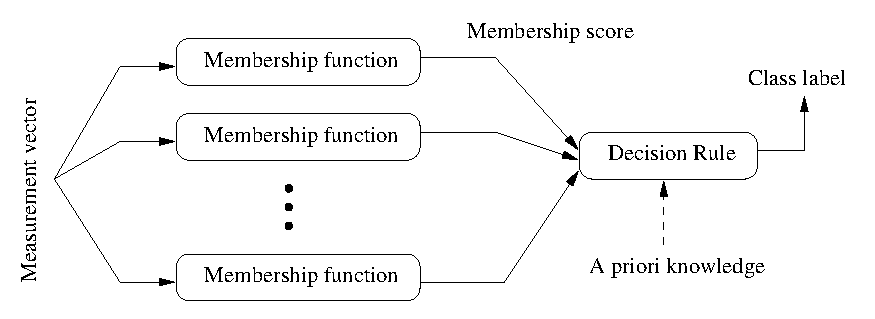
\includegraphics[width=0.7\textwidth]{DudaClassifier.eps}
  \itkcaption[Simple conceptual classifier]{Simple conceptual classifier.}
  \label{fig:simple}
\end{figure}

This framework closely follows that of Duda and
Hart\cite{Duda2000}. The classification process can be described
as follows:

\begin{enumerate}
\item{A measurement vector is input to each membership function.}
\item{Membership functions feed the membership scores to the
    decision rule.}
\item{A decision rule compares the membership scores and returns a
    class label.}
\end{enumerate}

\begin{figure}
  \centering
  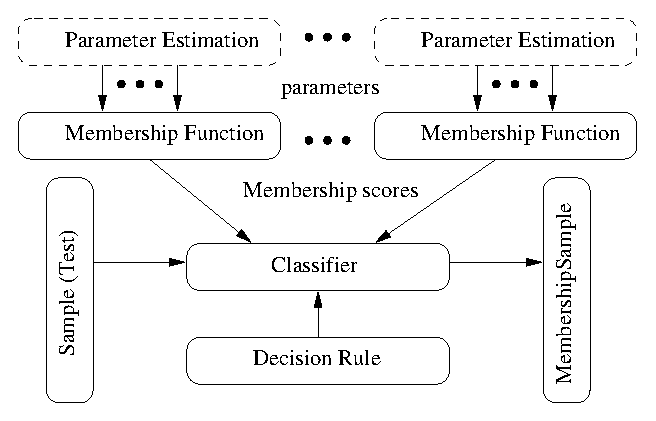
\includegraphics[width=0.7\textwidth]{StatisticalClassificationFramework.eps}
  \itkcaption[Statistical classification framework]{Statistical classification
framework.}
  \protect\label{fig:StatisticalClassificationFramework}
\end{figure}

This simple configuration can be used to formulated various classification
tasks by using different membership functions and incorporating task specific
requirements and prior knowledge into the decision rule. For example, instead
of using probability density functions as membership functions, through
distance functions and a minimum value decision rule (which assigns a class
from the distance function that returns the smallest value) users can achieve a
least squared error classifier. As another example, users can add a rejection
scheme to the decision rule so that even in a situation where the membership
scores suggest a ``winner'', a measurement vector can be flagged as ill
defined. Such a rejection scheme can avoid risks of assigning a class label
without a proper win margin.

\subsection{k-d Tree Based k-Means Clustering}
\label{sec:KdTreeBasedKMeansClustering}
\ifitkFullVersion
\input{KdTreeBasedKMeansClustering.tex}
\fi

\subsection{K-Means Classification}
\label{sec:KMeansClassifier}
\ifitkFullVersion
\input{ScalarImageKmeansClassifier.tex}
\fi

\subsection{Bayesian Plug-In Classifier}
\label{sec:BayesianPluginClassifier}

\ifitkFullVersion
\input{BayesianPluginClassifier.tex}
\fi


\subsection{Expectation Maximization Mixture Model Estimation}
\label{sec:ExpectationMaximizationMixtureModelEstimation}

\ifitkFullVersion
\input{ExpectationMaximizationMixtureModelEstimator.tex}
\fi

\subsection{Classification using Markov Random Field}
\label{sec:MarkovRandomField}

Markov Random Fields are probabilistic models that use the correlation between
pixels in a neighborhood to decide the object region. The
\subdoxygen{Statistics}{MRFImageFilter} uses the maximum a posteriori (MAP)
estimates for modeling the MRF. The object traverses the data set and uses the
model generated by the Mahalanobis distance classifier to gets the the distance
between each pixel in the data set to a set of known classes, updates the
distances by evaluating the influence of its neighboring pixels (based on a MRF
model) and finally, classifies each pixel to the class which has the minimum
distance to that pixel (taking the neighborhood influence under consideration).
The energy function minimization is done using the iterated conditional modes
(ICM) algorithm \cite{Besag1986}.

\ifitkFullVersion
\input{ScalarImageMarkovRandomField1.tex}
\fi


\backmatter

%%%%%%%%%%%%%%%%%%%%%%%%%%%%%%%%%%%%%%%%%
%
%  Insert the bibliography using BibTeX
%
%%%%%%%%%%%%%%%%%%%%%%%%%%%%%%%%%%%%%%%%%

\bibliographystyle{plain}
\bibliography{\bibtexdatabasepath}


%%%%%%%%%%%%%%%%%%%%%%%%%%%%%%%%%%%%%%%%%
%
%  Insert the Index file
%
%%%%%%%%%%%%%%%%%%%%%%%%%%%%%%%%%%%%%%%%%

\InputIfFileExists{001-ITKSoftwareGuide-Book2.ind}


%\ifitkPrintedVersion
%\cleardoublepage
%\newpage
\newpage
\thispagestyle{empty}
\includegraphics[width=14cm]{flyer-vtk-textbook.eps}
\newpage
\thispagestyle{empty}
\includegraphics[width=14cm]{flyer-cmake.eps}
\newpage
\thispagestyle{empty}
\includegraphics[width=14cm]{flyer-itk.eps}
\newpage
\thispagestyle{empty}
\includegraphics[width=14cm]{flyer-paraview.eps}
\newpage
\thispagestyle{empty}
\includegraphics[width=14cm]{flyer-activiz.eps}
\newpage
\thispagestyle{empty}
\includegraphics[width=14cm]{flyer-volview.eps}
\newpage
\thispagestyle{empty}
\includegraphics[width=14cm]{flyer-polyviz.eps}
\newpage
\thispagestyle{empty}
\includegraphics[width=14cm]{flyer-kitware.eps}

%\fi

\end{document}
